\documentclass[10pt,twocolumn,letterpaper]{article}

\usepackage{procams}
\usepackage{times}
\usepackage{epsfig}
\usepackage{graphicx}
\usepackage{amsmath}
\usepackage{amssymb}

% Include other packages here, before hyperref.

% If you comment hyperref and then uncomment it, you should delete
% egpaper.aux before re-running latex.  (Or just hit 'q' on the first latex
% run, let it finish, and you should be clear).
\usepackage[pagebackref=true,breaklinks=true,letterpaper=true,colorlinks,bookmarks=false]{hyperref}


\procamsfinalcopy % *** Uncomment this line for the final submission

\def\procamsPaperID{8} % *** Enter the PROCAMS Paper ID here
\def\httilde{\mbox{\tt\raisebox{-.5ex}{\symbol{126}}}}

% Pages are numbered in submission mode, and unnumbered in camera-ready
\ifprocamsfinal\pagestyle{empty}\fi
\begin{document}

%%%%%%%%% TITLE
%\title{ARmy: Multi-User Interaction in a Spatially Augmented Reality Game}
\title{ARmy: A Study of Multi-User Interaction in Spatially Augmented Games}

\author{Andrew Dolce\\
%Rensselaer Polytechnic Institute\\
%Institution1 address\\
{\tt\small andrew@gradientstudios.com}
% For a paper whose authors are all at the same institution,
% omit the following lines up until the closing ``}''.
% Additional authors and addresses can be added with ``\and'',
% just like the second author.
% To save space, use either the email address or home page, not both
\and
Joshua Nasman\\
%Institution2\\
%First line of institution2 address\\
%{\tt\url{http://www.author.org/~second}}
{\tt\small nasmaj@cs.rpi.edu}\\
{\normalsize Department of Computer Science \vspace{-0.01in}}\\
{\normalsize Rensselaer Polytechnic Institute} 
\and
Barbara Cutler\\
{\tt\small cutler@cs.rpi.edu}
%\begin{center}
%{\centering
%\end{center}
}

\maketitle
% \thispagestyle{empty}

%%%%%%%%% ABSTRACT
\begin{abstract}
%Augmented reality offers a means of overlaying interactive virtual
%elements onto real world environments.  Further motivated by
%an interest in
%developing new methods for 
%natural multi-user interactions in the context of games, 
\vspace{-0.1in}
We present
\emph{ARmy,} 
%a proof of concept, 
a two-player military strategy game 
%\fbox{proof of concept}
that 
%demonstrates the
%concept of 
uses spatially augmented reality to combine physical tabletop games
with the virtual elements and computation characteristic of modern
video games.  
%
As players move plastic miniatures within a small scale physical
environment, the application moderates and augments play by
maintaining a 3D representation of the scene, which it uses to
validate movement paths and perform automatic line-of-sight
calculations for combat.
%
%The ARmy application 
%leverages a {\em table-top Spatially Augmented
%  Reality} system 
%is built on top of a display system capable of
%dynamically augmenting the appearance of physical objects.  The system
%uses 
%with a single overhead camera to track a collection of movable, white
%surfaces, and applies virtual textures to these objects using six standard office 
%$multiple
%projectors.  
%We describe some of the implementation details,
%advantages, and limitations of the application. 
We describe the design and implementation of the ARmy gaming system.
Furthermore, we conducted a user study
%In addition, we studied users interacting with the
%system 
to gauge the effectiveness, intuitiveness, and robustness of the
application.  We describe the process of this user study, present
quantitative data of the study results, and discuss general design
principles for the design and implementation of other engaging
spatially-augmented games.
%We performed 
%\fbox{add a bit more about the user study}
%
\vspace{-0.1in}
\end{abstract}

%%%%%%%%% BODY TEXT
\section{Introduction}

Games are found throughout every day life in a variety of forms, and
can be a source of entertainment, a means for education, and even a
medium for artistic expression or social commentary.  Tangible
``tabletop games'' include a variety of board, card, and dice games,
such as chess, \emph{Monopoly},
%~\cite{Monopoly} 
\emph{The Settlers of Catan}, and
%~\cite{Catan}, 
%\emph{Puerto Rico}~\cite{PuertoRico},
\emph{Magic: The Gathering}.
%, and
%~\cite{MTG}, 
%\emph{Dungeons \&  Dragons}~\cite{D&D}, 
%\emph{Warhammer 40,000}~\cite{Warhammer40k}.  
%
These games use physical pieces to facilitate play.  
Modern video games provide an experience that is purely virtual,
allowing the user to interact with a virtual game world that can
%responds
%in realtime with appealing visuals. Video games have the advantage of
%being autonomous agents, allowing for the incorporation of 
include complex simulations and automatic rules enforcement. In
contrast, tabletop games hold players responsible for moderating play,
which can be difficult and tedious. However, the physically
tangible interfaces of tabletop games are often preferable to
electronic input devices, which can be challenging and alienating to
novice users.

% FIGURE SHOWING GENERIC PLAYING / POINTING
\begin{figure}[t]
\newcommand{\picwidth}{1.625in}
\resizebox{\picwidth}{!}{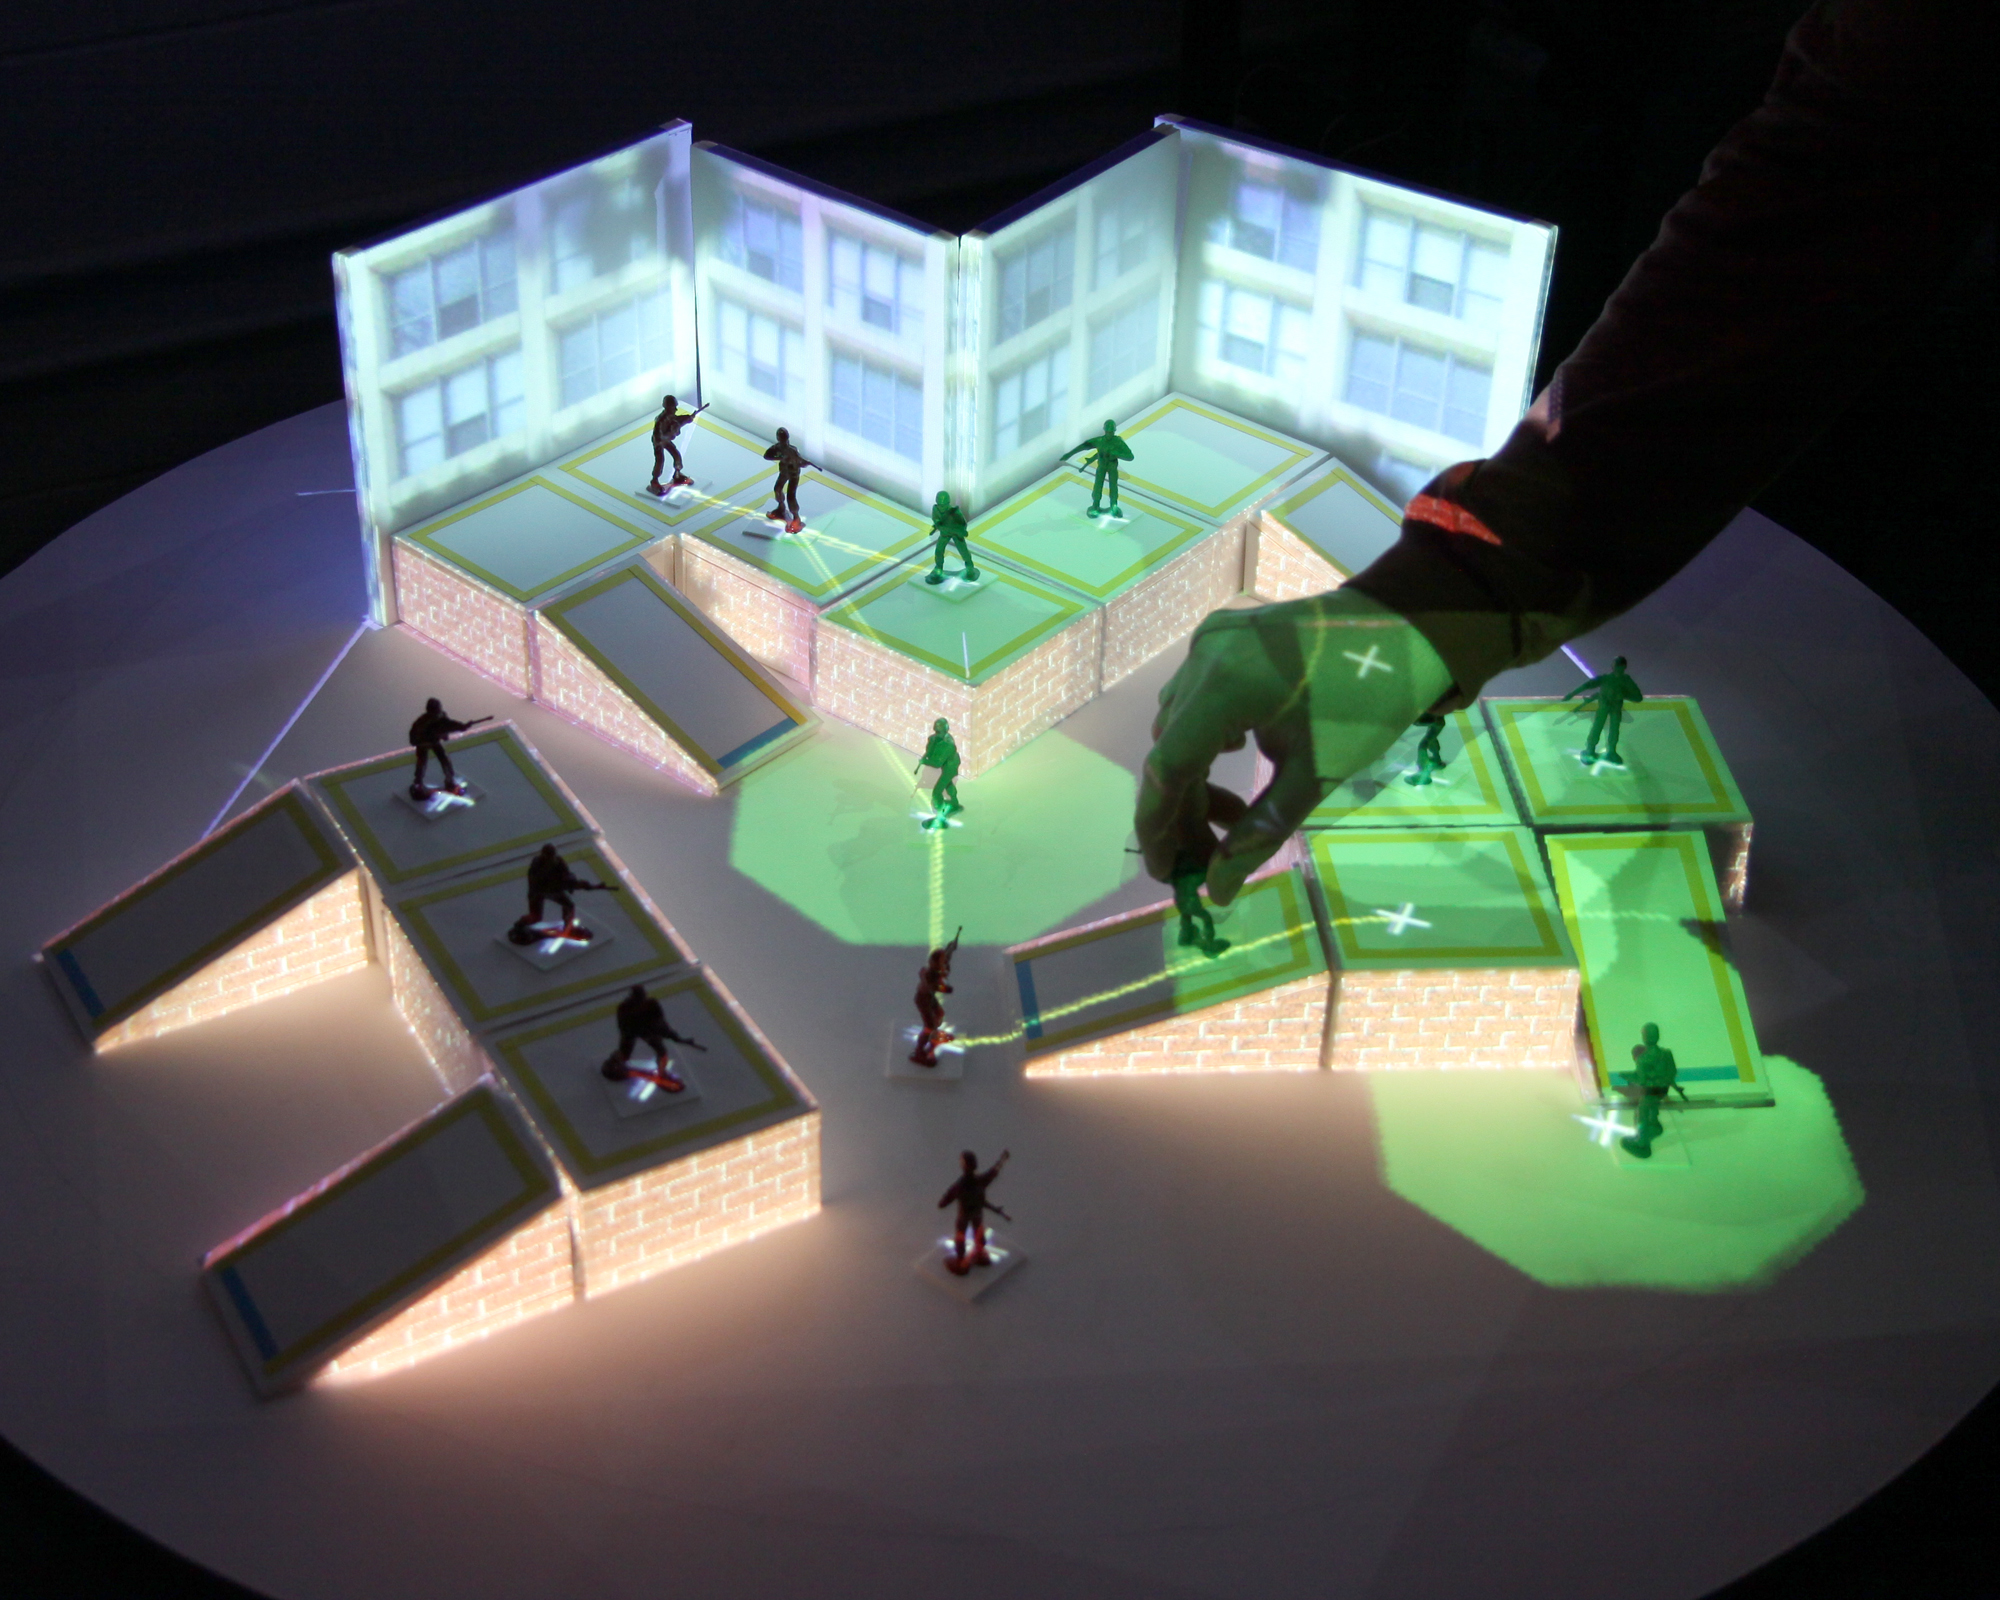
\includegraphics{../gi2012_army/images/greens_move_3.jpg}}
\resizebox{\picwidth}{!}{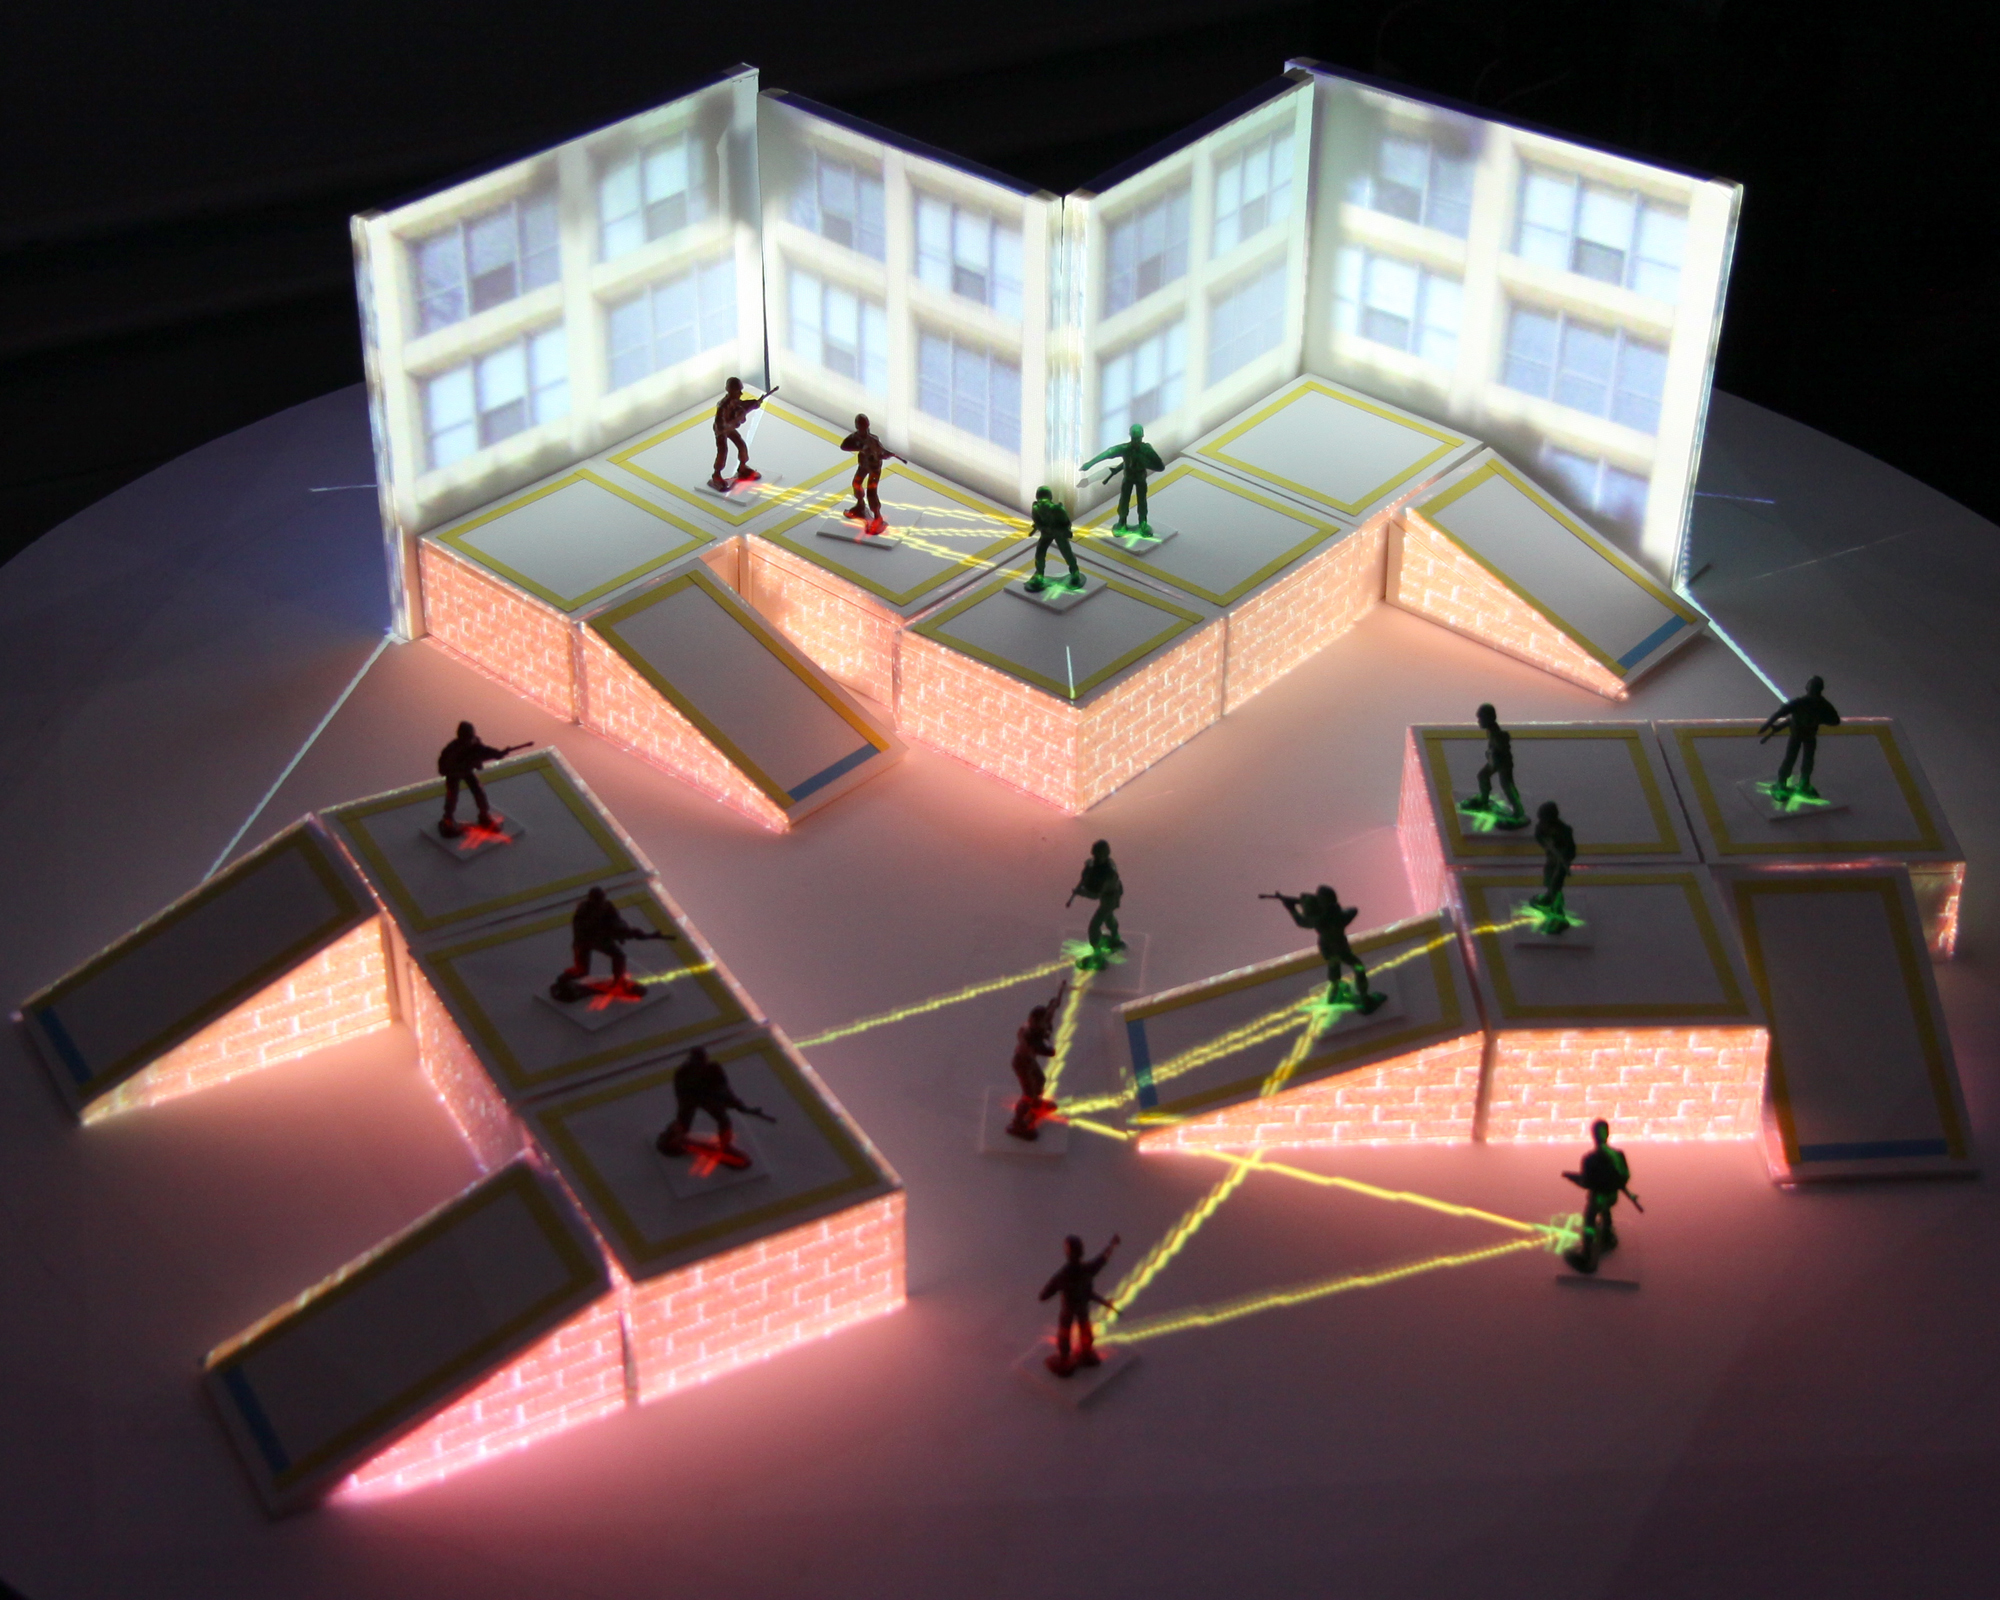
\includegraphics{../gi2012_army/images/lots_of_combat_2.jpg}}\\
\resizebox{\picwidth}{!}{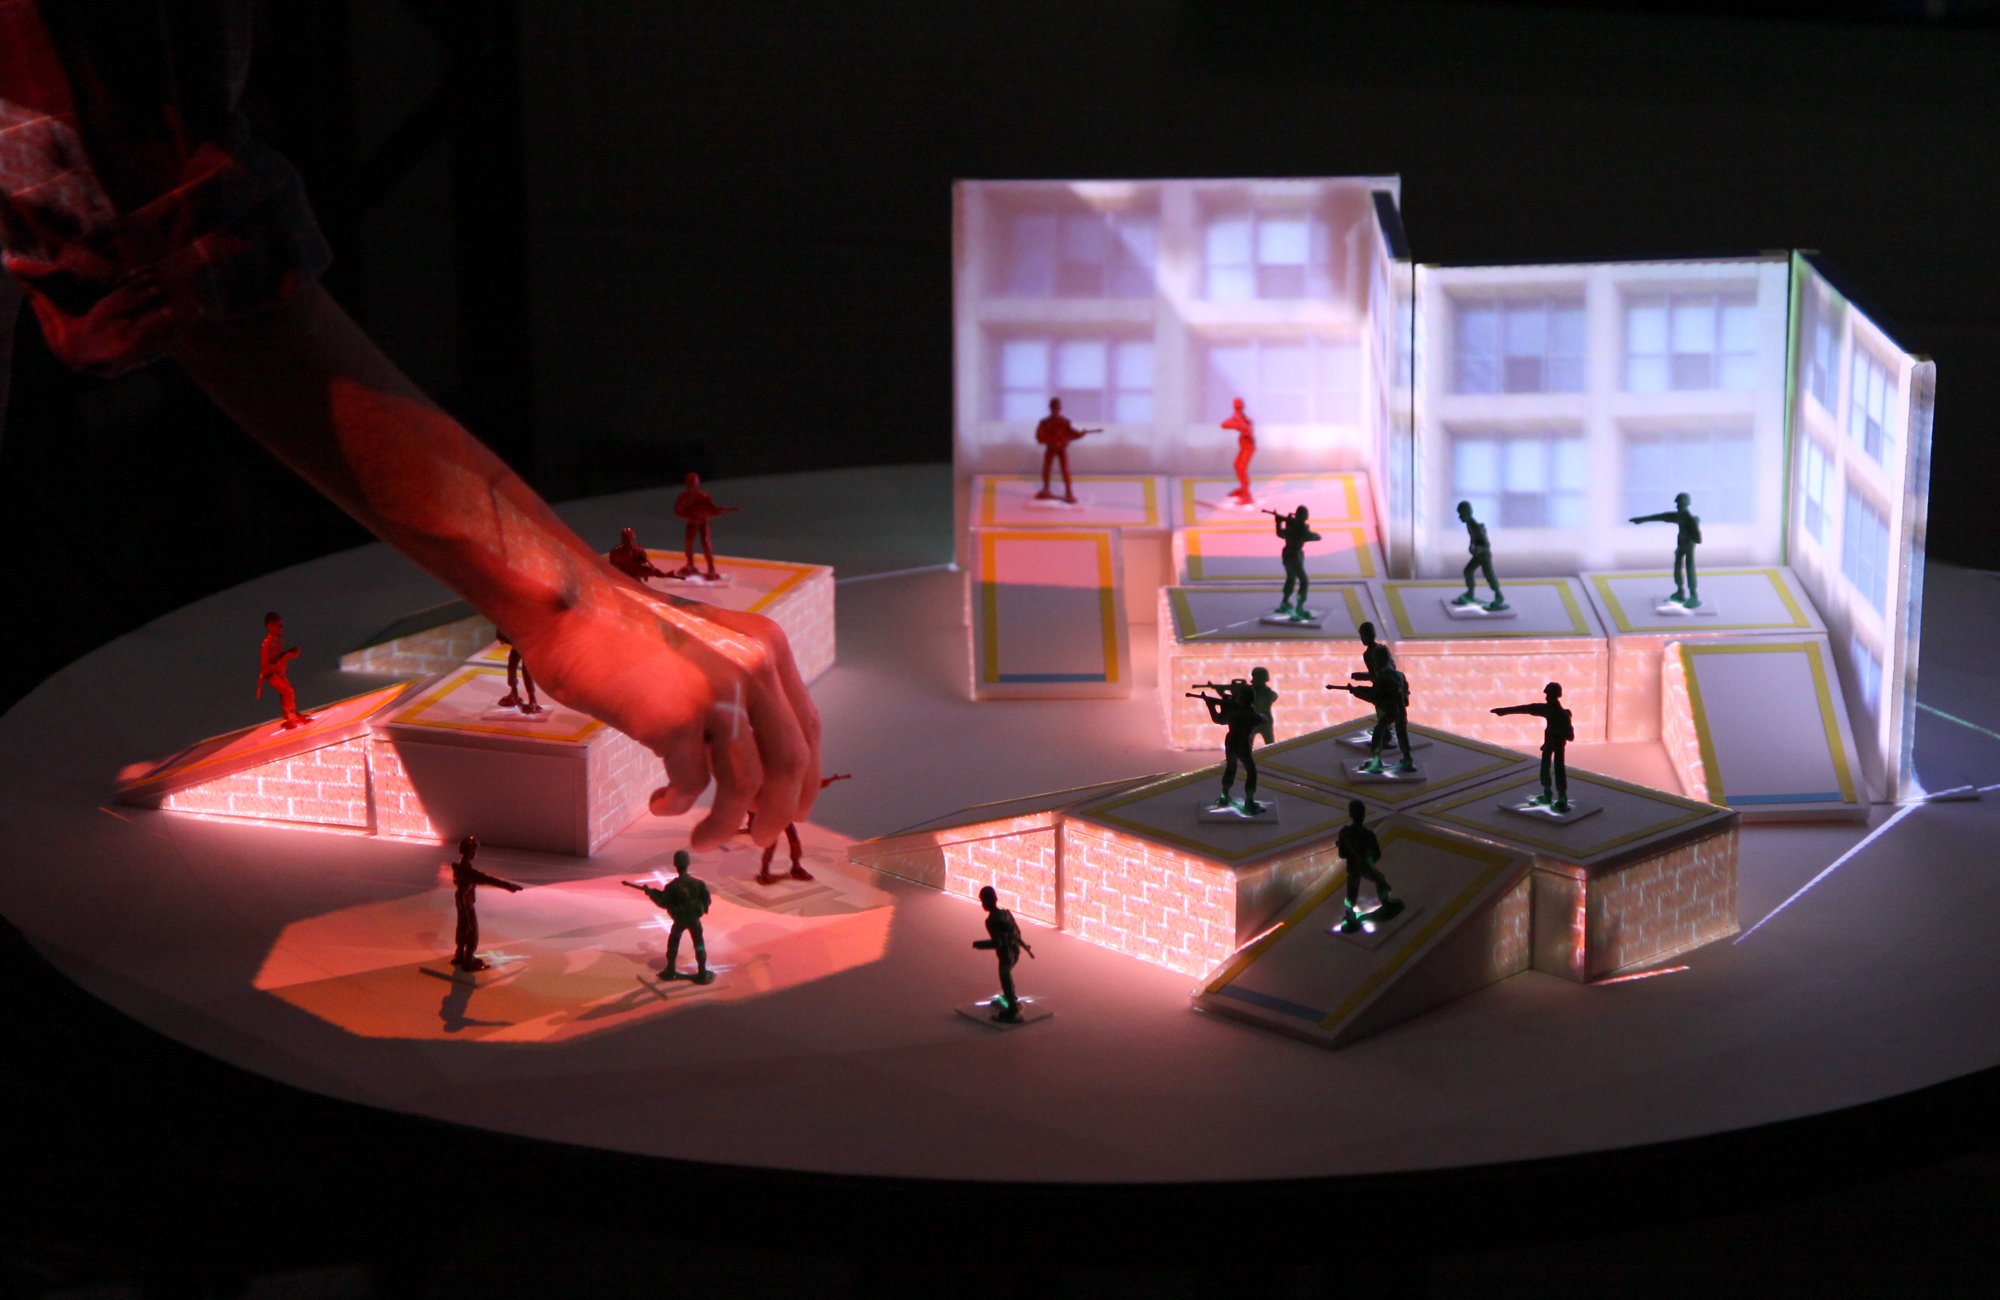
\includegraphics{../gi2012_army/images/reds_move.jpg}}
\resizebox{\picwidth}{!}{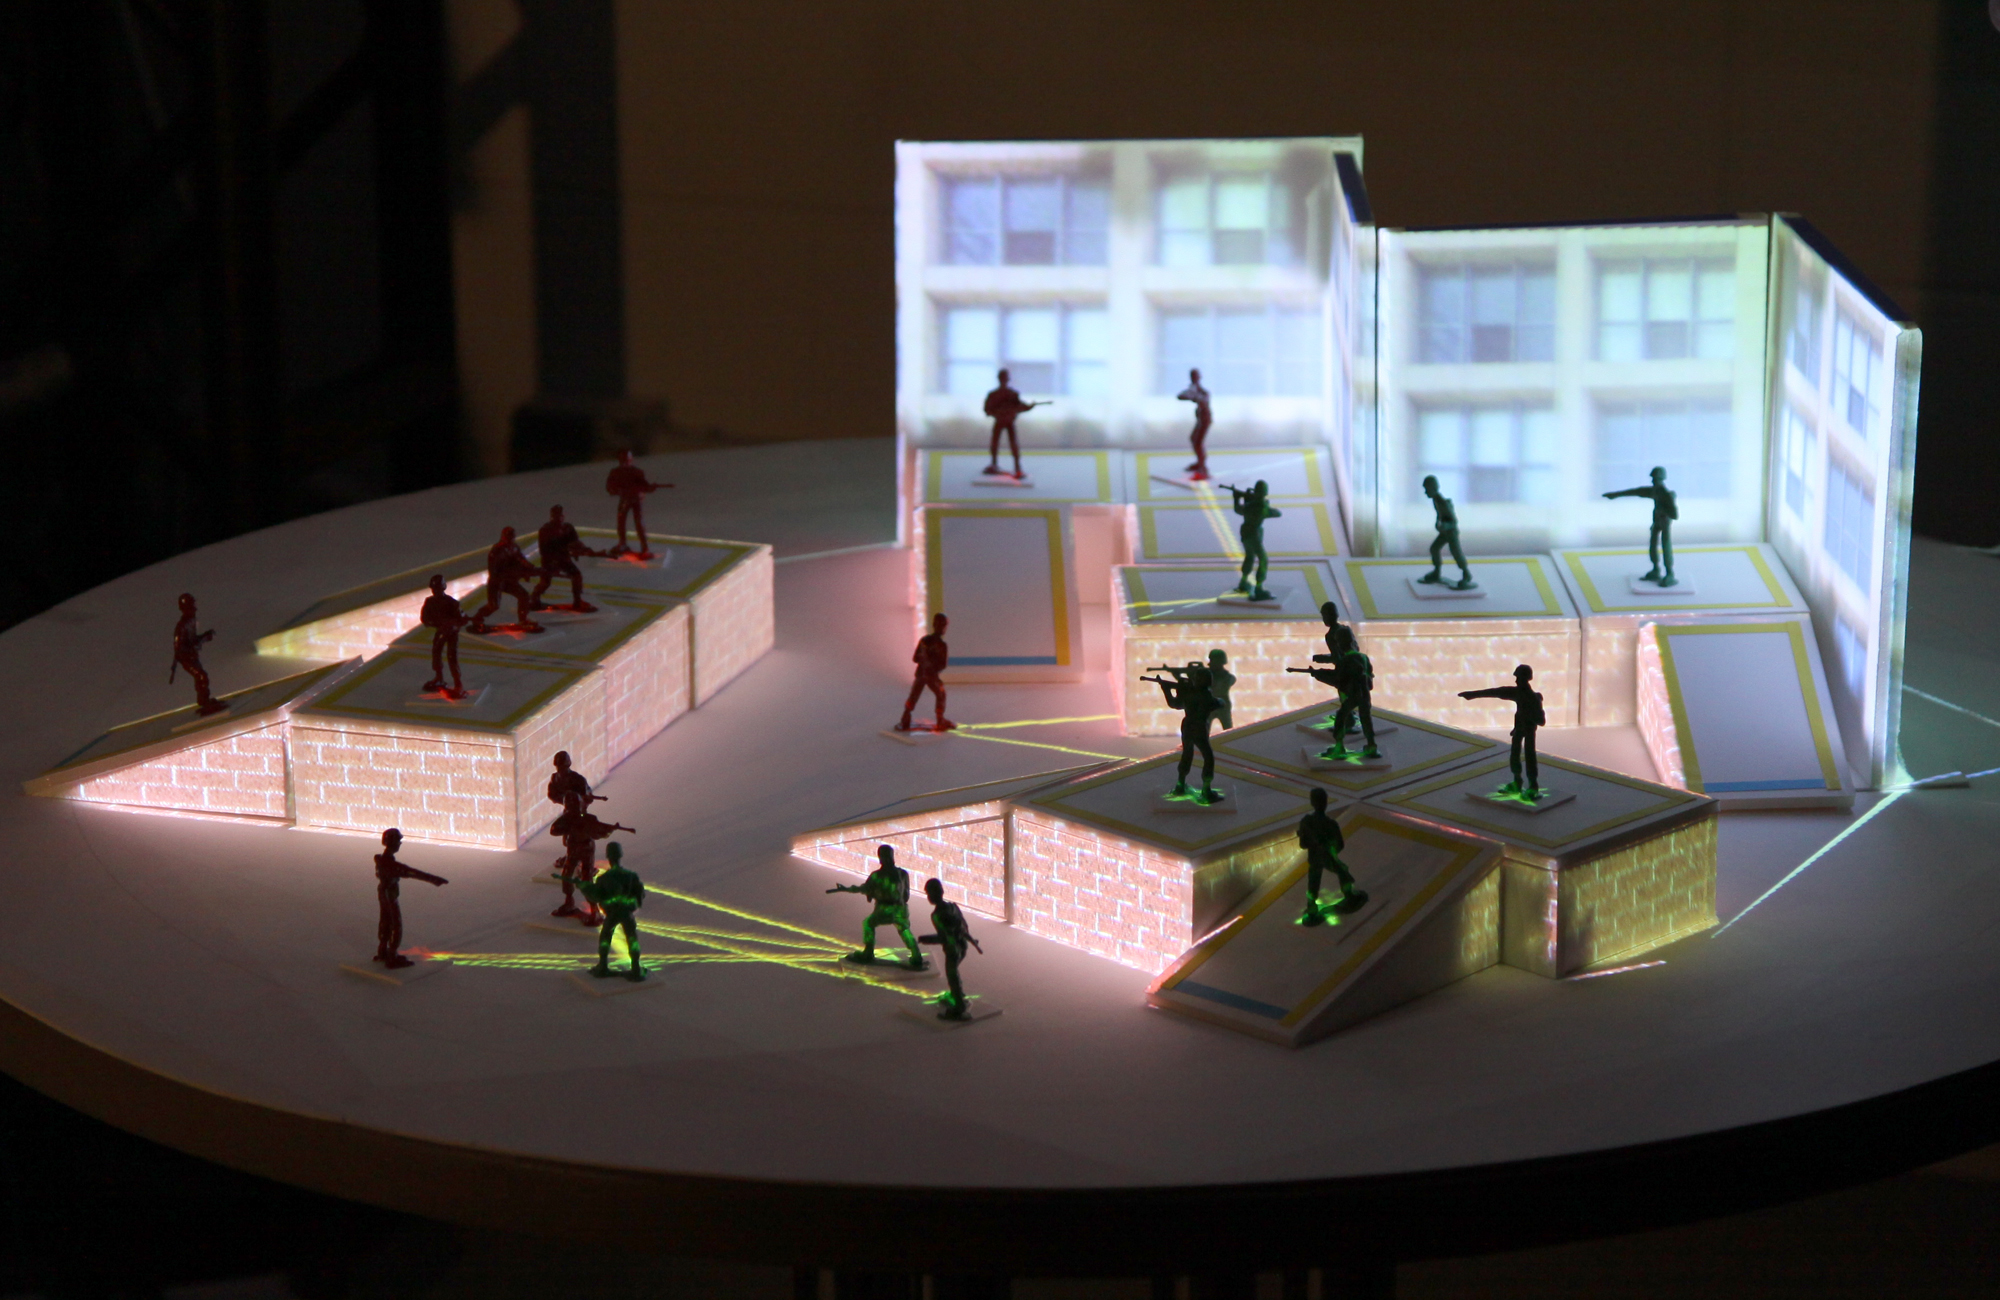
\includegraphics{../gi2012_army/images/lots_of_combat.jpg}}%
%\vspace{-0.2in}\\
\caption[Images of ARmy: A Spatially Augmented Reality Game]{ The
  \emph{ARmy} game is an example of a spatially augmented reality game
  that combines physical game objects with virtual elements through
  projection.  The projections decorate simple, white objects with
  colorful virtual textures, and display important game information
  regarding legal moves and simulated combat.  }
\label{FIGURE:GameInProgress}
\vspace{-0.15in}
\end{figure}

%Recent strides in The field of 
Augmented Reality (AR) has opened up new, exciting and engaging ways
for users to view and interact with virtual elements embedded in the
real world.
%.  Our work
%is motivated by the possibility of AR games that combine elements of
%tabletop games and video games to create an exciting, new experience.
We present \emph{ARmy} (Figure~\ref{FIGURE:GameInProgress}), an AR
miniature war game played using plastic soldier figurines and physical
terrain models in a style similar to \emph{Warhammer
  40,000}~\cite{Warhammer40k}.  Multiple projectors are used to
directly augment the play surface, displaying useful information about
the game state and adding visual detail to the terrain.  An overhead
camera tracks the movements of the game pieces, and a semi-autonomous
game module maintains game state and moderates play. This ensures
that the rules are correctly followed and removes the need for players
to perform tedious bookkeeping tasks, such as measuring distances or
rolling dice to resolve outcomes.

\vspace{0.05in}
\noindent
Our contributions presented in this paper:\vspace{-0.1in}

\begin{itemize}

\item Design a robust implementation of a tabletop spatially augmented
  multiplayer war strategy game.\vspace{-0.1in}
  
\item A user study demonstrating:\vspace{-0.12in}

\begin{itemize}

\item Improved efficiency of our projector augmented version of the game over
  the traditional non-augmented version.\vspace{-0.05in}

\item Accurate, unbiased, and unambiguous enforcement of game
  rules. \vspace{-0.12in}

\end{itemize}

\item General guidelines for the creation of other engaging spatially
  augmented games.

%Not sure this bullet adds anything
%\item Evaluation of the effectiveness of the \emph{ARmy} game in
%  combining the advantages of tabletop games and video
%  games.\vspace{-0.1in}


\end{itemize}

%We briefly survey some of the related work, both in relation to games
%and AR in general.  We describe the game play and interface of ARmy, and
%briefly discuss the underlying details of our multiprojector system.
%We detail the process of running user studies on the system, and
%discuss the results of the studies in relation to our goals.  Finally,
%we discuss current limitations of the system, as well as improvements
%to be made through future work.


\section{Related Work}
\label{section:related_work}

% in Augmented and Tangible Interface Design and Implementation}

%Augmented reality is a relatively recent field, with a large amount of
%research focusing on how to combine the underlying technologies to
%achieve stable, reproducible systems.  

The technological challenges in augmented reality systems
%that these
include the creation of effective augmented displays, 3D
registration and tracking, and tangible interaction.


%\subsection{Immersive Display Technology}

\vspace{-0.15in}
\paragraph{Immersive Display Technology} 

%
Existing AR systems use a variety of display techniques,
%, which Bimber
%and Raskar
which are classified~\cite{BimberBook} into three main groups:
head-mounted, hand-held, and spatially aligned.
%
Head-mounted displays
are devices physically worn by the user, e.g.,
%Sutherlands's~
an optical see-though display~\cite{Sutherland1968}.  Hand-held
displays use 
%ubiquitous technology, such as 
%Personal Digital
%Assistants (PDAs), 
smart phones or handheld game consoles
%personal video game platforms
for video see-through
techniques~\cite{Pasman2003, Wagner2003, Nintendo3DS}.  
%Recent work has produced
%examples of hand-held AR video games, such as
For example, the \emph{ARhrrrr!}
game
%a game
%developed by the Georgia Tech Augmented Environments Lab and the
%Savannah College of Art and Design  The game is
is played on a mobile device that overlays graphics onto a physical
paper map, and uses tangible, brightly colored
candies as input props~\cite{ARhrrrr!}.
%A fully commercialized example of hand-held AR is the
%Nintendo 3DS~\cite{Nintendo3DS}, which offers mobile AR games on an
%autostereoscopic screen.
%
Spatially aligned techniques create displays physically aligned with the environment,
%\fbox{more the 2nd class than SAR?}
%Some spatial displays 
%may apply optical or video-based see-through
%techniques 
%by using stationary screens or monitors. For example,
% Bimber et
%al. present a 
%the ``Virtual Showcase'' uses half-silvered mirror combiners 
%to create an enclosed 
such as the ``Virtual Showcase'' display~\cite{Bimber2005}.
%an enclosed AR display analogous to the physical showcases typical of
%museum exhibits~\cite{Bimber2005}.
%
%
The {\em ARmy} game is an example of \emph{Spatially Augmented
  Reality} (SAR)~\cite{BimberBook},
%, a
%term coined by Bimber and Raskar
%to describe AR
a class of AR systems where the display devices are physically 
%aligned
%and 
embedded in or projected onto the real-world environment.
%, instead of being attached to the user.  
%More closely related to our research are techniques which directly
%augment the surfaces of physical objects using some configuration of
%video projectors. An important and well-known example is the 
%CAVE
%``CAVE Automatic Virtual Environment'', 
%developed by
%Cruz-Neira et. al
These environments can surround and immerse the user with large-scale
projections~\cite{Cruz-Neira1993,Raskar1998a}. 
%,Raskar1998b}.  
%, e.g., the CAVE
% Although the CAVE is technically
%classified as an example of virtual reality, it stands as a
%significant precursor to SAR techniques.  The display area is an
%enclosed room comprised of rear-projection screens and a top-down
%projector for displaying images on the floor, thus allowing for an
%effective immersive environment.  The user is equipped with
%head-tracking devices and 3D goggles for stereoscopic image display.
%
%Raskar et. al present 
%and ``Office of the Future''~\cite{
%, which
%explores the possibility of using SAR applications in the setting of
%an everyday workspace to facilitate telepresence and computing
%tasks
%They used 
%Multiple projectors present images on irregular, nonplanar surfaces,
%and demonstrated a technique for generating images suitable for such
%displays~\cite{Raskar1998b}.
%Their 
Alternatively, 
%Later work expands upon 
these techniques can be applied at a table-top scale
%with the idea of ``Shader
%Lamps'', which allow for augmentation of 
%complex 3D objects 
giving complex 3D objects
%creating
%to create
%the 
new appearance properties~\cite{Raskar2000}. 
%appearance of desired material properties, such as color and
%texture
%
%
A 
%significant 
theme for 
%much 
projection-based SAR research is 
%the
%vision of 
a future in which these 
%display 
technologies 
%have 
become
truly 
ubiquitous~\cite{Underkoffler1999,Pinhanez2001}.   
% .  
%Underkoffler et al.  presented the idea of a
%e.g., the ``Luminous Room''
% is lit by multiple ``IO bulbs'', which combine a
%projector and camera to facilitate both spatial display and user
%interactions~\cite{Underkoffler1999}.  
%Pinhanez proposed the use of
%and ``Everywhere Display'' projectors~\cite{Pinhanez2001}.  
%equipped with poseable mirrors allow
%for the projection to be steered to any suitable surface within the
%surrounding environment~\cite{Pinhanez2001}.  




\vspace{-0.15in}
\paragraph{3D Registration and Tracking} 
%\fbox{\& DETECTION?}

%\fbox{ more tui, less tracking?}
%\fbox{perhaps cut to a paragraph} 
%\fbox{cite us (and other ref) for color tracking?   mention other methods in passing?}

The virtual game elements and tangible input devices must be aligned
and tracked within a common 3D physical environment.  
%This involves
%two main steps: calibration and tracking.
%
%\subsubsection{Calibration}
%
%Calibration refers to the problem of correctly modeling and recovering
%geometric correspondences between display or tracking devices and the
%physical environment.
%% In the case of projector-based displays, it is necessary that we be %% able to map each projector pixel to a known point relative to the %% world coordinate system so that we can use that information to project %% images that are correctly aligned with the physical display surfaces.  %% In addition, since camera devices are required for vision-based %% techniques used in the tracking step, these devices must also be %% calibrated.
%Camera and projector calibration is a classic vision topic that has
%been researched thoroughly.  
%Typically cameras and projectors are described using the pinhole
%model, which maps 3D points in the world to 2D image coordinates using
%both intrinsic parameters, which describe center, scale, and skewness
%of the image coordinate system, and extrinsic parameters, which
%describe the rotation and translation of the camera relative to world
%coordinates.  
One or more fixed cameras placed in the physical environment may be
calibrated to a common world coordinate system~\cite{Zhang2000}.
%of fixed cameras placed in the physical environment.
%^Zhang
%provides a simple, robust method for
%calibration 
%in which the user captures multiple images of a single,
%
%planar calibration target from differing points of view.  The method
%requires no a priori knowledge of the position, orientation, or
%movement of the target relative to the camera.
%Additional research
%Scaramuzza et al.~\cite{Scaramuzza2006} focus on recovering
%Calibration parameters involving significant lens distortion,
%specifically omnidirectional cameras, as well as cameras equipped with
%a fisheye lens.
%
%\subsubsection{Tracking}
%
The image data from these cameras can then detect, monitor, and track
physical objects allowing them to interact with and direct the virtual
world in real-time.
% Once the display and vision
%devices are properly calibrated within the world coordinate system, we
%can use them to accomplish tracking of physical objects for
%augmentation.  Unlike calibration routines, which typically are done
%once during setup, and therefore can accommodate somewhat
%time-consuming, manual tasks, tracking must be done automatically and
%efficiently at interactive rates for the system to be responsive.
%Registration and tracking can be accomplished using electromagnetic
%and mechanical tracking devices~\cite{Cruz-Neira1993} or using a
%variety of vision-based techniques.  \fbox{out of  order... }
%, which are discussed below.
%
%% \paragraph{Fiducial Markers}
%
%
A large variety of AR applications use fiducial markers to identify
objects and determine their position and orientation~\cite{Kato1999,
  Fiala2005}.
%Kato and
%Billinghurst~\cite{Kato1999} provide a method for tracking square,
%planar markers with a black border and bi-tonal interior pattern.
%Their method identifies markers in the camera image by using
%edge-based vision techniques to detect quadrilaterals.  Detected
%regions are normalized, sampled, and compared via correlation to a set
%of marker patterns provided a priori by the user.  
%They present their
%technique in the context of an augmented reality conferencing system,
%This software was released as ARToolkit, and has since become
%well-known and widely used within the AR community.  ARTag, a similar
%quadrilateral-based method developed by Fiala~\cite{Fiala2005}, uses
%an extensive library of predefined marker codes to achieve increased
%robustness in cases of partial occlusion. 
%\fbox{ Added stuff
%  here... should I have?}
%employs digital processing techniques to identify square markers
%bearing ten-digit identification codes, encoded in the form of
%six-by-six bitonal grids similar to barcodes.  This tracking system,
%known as ARTag, provides the user with a large library of predefined
%markers, and leverages redundancies in the encoding technique to
%identify markers even under conditions of partial occlusion.
%
%Fiducial marker systems hold great promise for AR game applications,
%as they provide a viable, inexpensive means of identifying specific
%game-related objects.  
%For example, markers could be printed on cards,
%attached to wooden game pieces, or positioned at the corners of a
%movable game board.
% in a manner similar to the augmented whiteboard
%used in Kato and Billinghurst's conferencing system~\cite{Kato1999}.
However, the robustness and accuracy of the tracking depends
on the relative size of these markers.
% in the camera image.
%, since an image of a marker that is too
%small or far away may not yield sufficient resolution for the tracking
%algorithm to identify the contained pattern.  
%Thus, suitable tracking may 
%These 
%require 
Sufficiently sized tokens may be
%come
%that are 
too large 
%or
%unwieldy 
for players to use comfortably
%.  In addition, large fiducial
and 
%markers 
may interfere with the visual quality of virtual elements projected
onto them.  Unlike see-through AR displays, projector-based SAR
systems cannot fully hide the marker with rendered objects.

We have chosen to detect and track the game pieces in ARmy using
application-specific colors, shapes, and patterns, similar
to~\cite{Underkoffler1999}.
%Underkoffler et al.
%
Color-based object recognition is appropriate for augmenting the play
of many existing board and card games which have distinctive,
brightly-colored elements, allowing detection and tracking without
modifying the game pieces.
% This allows us to color-based object recognition may be useful in
%the context of SAR games, since color is commonly used in board and
%card games to distinguish objects that appear otherwise identical.
%Thus it might be possible to track existing game pieces without the
%need for additional annotation.
However, color-based techniques can be problematic with inconsistent
lighting conditions and background clutter.
%,
% and are likely to
%suffer from a high number of false positives, as target colors may
%appear within background clutter.  Despite these drawbacks,
%
Alternative methods for interactive 3D tracking include
electromagnetic and mechanical tracking~\cite{Cruz-Neira1993},
structured light~\cite{Ashdown2004,Lee2004}, and
infrared~\cite{Lee2007,Kinect,Maimone12}.


%Other useful methods for 3D registration employ structured light
%techniques, which project known pixel patterns into the scene and
%measure the result in order to recover depth
%information~\cite{Ashdown2004,Lee2004}.
%Ashdown et
%al. use a variation of structured light to project
%successive patterns containing continuous horizontal and vertical
%lines.  
%The method detects ``kinks'' in the lines and uses this
%information to segment the image into multiple planar regions, which
%are then stitched together into a continuous display by refining their
%individual homographies to fit adjacency constraints.  
%Lee et al.~\cite{Lee2004} propose a structured light method for
%registering projection surfaces 
%without the use of a camera and vision
%techniques.  Instead, 
%by embedding light sensors in the corners of the target surface
% are embedded
%The sensors detect patterns projected onto the surface and
%with light sensors, which detect and transmit the binary sequences
%projected in the patterns.  The system 
%use this information to track the 3D position of the object.
%identify the quadrilateral region of the
%surface within the projector image and warps images accordingly.

%% \paragraph{Imperceptible Pattern Embedding}

%% A potentially serious hurdle for the application of fiducial marker %% and structured light techniques to display systems that use direct %% augmentation is interference from projected images.  In other words, %% projecting a colored image onto a surface bearing a fiducial marker %% may obscure the pattern of the marker in such a way as to prevent %% correct identification by the tracking algorithm.  Projected structured %% light patterns suffer from the same problem, and may obstruct the %% displayed images or otherwise distract the user.  

%% One possible solution to this problem involves directly embedding %% structured light patterns into the display images in such a way as to %% remain imperceptible to the user.  Lee et al.~\cite{Lee2005} %% demonstrate an improvement on their previous sensor-based technique %% which is able to embed the light patterns into perceptually uniform %% gray blocks, which are less distracting than high-contrast patterns.  %% Although the method is shown to achieve accurate tracking at %% interactive framerates, regions bearing the embedded patterns are %% still visible to the user and reduce the overall display space %% available for application content.  In addition, the method is shown to %% work only with a modified projector that outputs grayscale images.

%% Cotting et al.~\cite{Cotting2004} propose a method that achieves %% direct pattern embedding by taking advantage of unmodified DLP %% projectors, which use precisely-timed modulation of micro-mirrors to %% determine the intensity and color of each image pixel.  Each pixel %% corresponds to a single mirror, which switches between a ``white'' %% position that tilts toward the projector light source, thus %% contributing high intensity light to the image, and a ``black'' %% position that tilts away, thus contributing little light.  Their method %% first measures the sequences of mirror flips across the full range of %% color values for each independent color channel.  Then it remaps each %% pixel to a perceptually similar color value such, that during a %% predetermined exposure time, the mirror's position matches the %% specified black or white value of the desired light pattern.  Using %% carefully calibrated exposures, the camera can acquire images of the %% light pattern without greatly degrading the image quality of the %% simultaneous display.  Although appealing, short-exposure methods such %% as this require the extra work of precisely synchronizing the camera %% and projectors.

%% \paragraph{Infrared Tracking}

%With SAR systems, vision-based tracking techniques often encounter a
%problem when projected images interfere with object tracking. One
%solution is to track objects with infrared light,
%based only on specific wavelengths of
%light which are not projected in significant amounts by the display.
%A significant amount of research has experimented with tracking using
%infrared light,
%which is invisible to the human eye and therefore does not interfere
%with displayed images~\cite{Lee2007,Kinect}.

%have
%presented the use of a hybrid LED projector capable of transmitting
%both infrared and visible light in order to simultaneously display
%visible application images and invisible structured light patterns.
%Although an excellent proof of concept, the proposed method does not
%work with standard commodity projectors.
%
%More recent work has led to the development of commercially available
%3D range cameras, which use infrared structured light techniques to
%produce real-time depth images of a measured scene.  Perhaps the most
%widely known example of this kind of registration is Microsoft's
%Kinect, a recent Xbox 360 peripheral that uses a depth-image camera as
%an input device for motion-based controls~\cite{Kinect, Shotton2011}.
%A different approach to infrared-based tracking is to use more
%conventional infrared-emitting devices, such as LED markers or laser
%pens.  Kato and Billinghurst demonstrated the use of an infrared
%LED-tipped stylus that allowed users to interact with a virtual
%whiteboard~\cite{Kato1999}.  The LED activates in response to pressure
%on the tip of the stylus, and is detected by a calibrated infrared
%camera.  Because the surface location of the whiteboard is known, the
%system is able to determine the location of the pen tip in screen
%coordinates, allowing the user to write or draw on the augmented
%display.
%
%\paragraph{Color-based Tracking}
%
%Finally, color information provides another potential means for detecting and
%registering objects.  For example, the Luminous Room project.~\cite{Underkoffler1999} 
%presented
%by Underkoffler et al
%used a simple tagging system through which application-specific
%objects were marked with small groupings of colored dots.  The system
%identifies objects by first detecting dots as regions of specified
%size and color, and then by grouping individual dots based on patterns
%with known distance and angle constraints.

%\fbox{add our color tracking here?}
%% An advantage of color-based techniques is that they are generally %% simpler to implement and at times faster than more sophisticated %% vision algorithms.  




%One problem of color-based techniques is that they may not be highly
%robust under inconsistent lighting conditions, and are likely to
%suffer from a high number of false positives, as target colors may
%appear within background clutter.  
%The Luminous Room prototype avoids
%these problems by using special reflective dot markers which appear
%brighter in the camera image, allowing them to be easily separated
%from the background.  In addition, colored markers share the same
%problem as bitonal fiducial markers, in that projected visuals are
%likely to obscure the appearance of the marker, making it difficult to
%achieve simultaneous capture and display.  
%Despite these drawbacks, color-based object recognition may be useful
%in the context of SAR games, since color is commonly used in board and
%card games to distinguish objects that appear otherwise identical.
%Thus it might be possible to track existing game pieces without the
%need for additional annotation.

% \paragraph{Human Tracking}

%% In addition to tracking physical game pieces, another set of %% interactions can be achieved through the tracking of the users.  
%% For example, the Kinect tracks the user's body and maps it to a %% skeleton model in real time, allowing for game applications to use %% full-body gestural controls~\cite{Shotton2011, Kinect}.  Other research %% has tried to achieve accurate tracking of specific body parts, most %% commonly focusing on the human hand.  Lee and H\"{o}llerer present %% Handy AR, a system for markerless tracking that detects and estimates %% the 3D pose of an out-stretched human hand~\cite{LeeT2007}.  This %% provides the benefit of allowing the user's hand to act in place of a %% fiducial marker, but requires the hand to remain out-stretched during %% use.  More recently, Wang and Popovi\'c~\cite{Wang2009} have proposed %% using a lightweight colored glove to allow for more robust detection %% of a wide variety of hand poses, including such complex gestures as %% the alphabet used in American Sign Language.








\begin{figure}[t]
\newcommand{\picwidth}{1.625in}
%\resizebox{!}{\picheight}{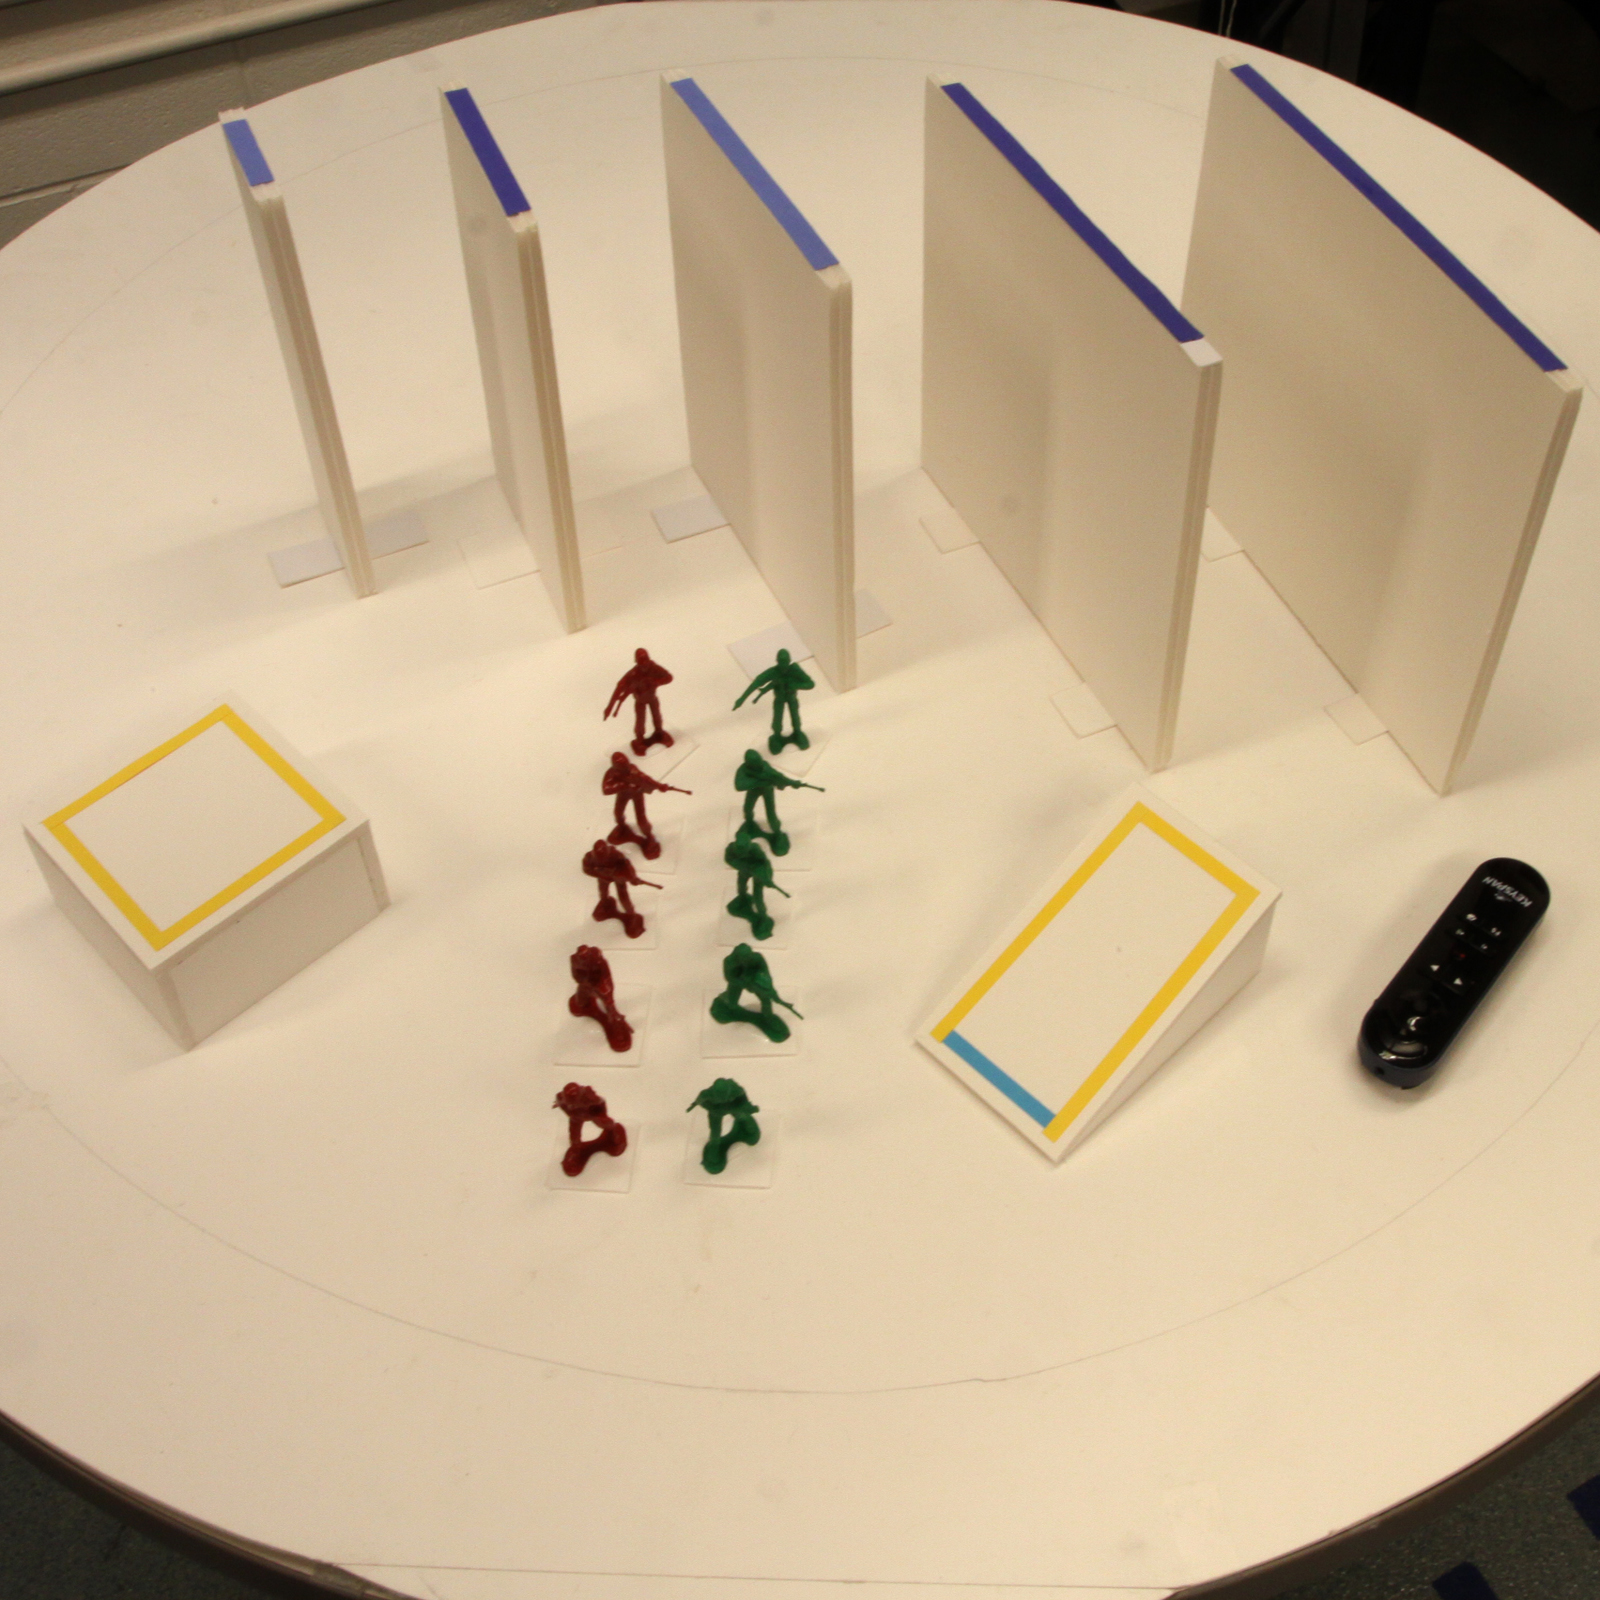
\includegraphics{images/props_crop.jpg}}
\resizebox{\picwidth}{!}{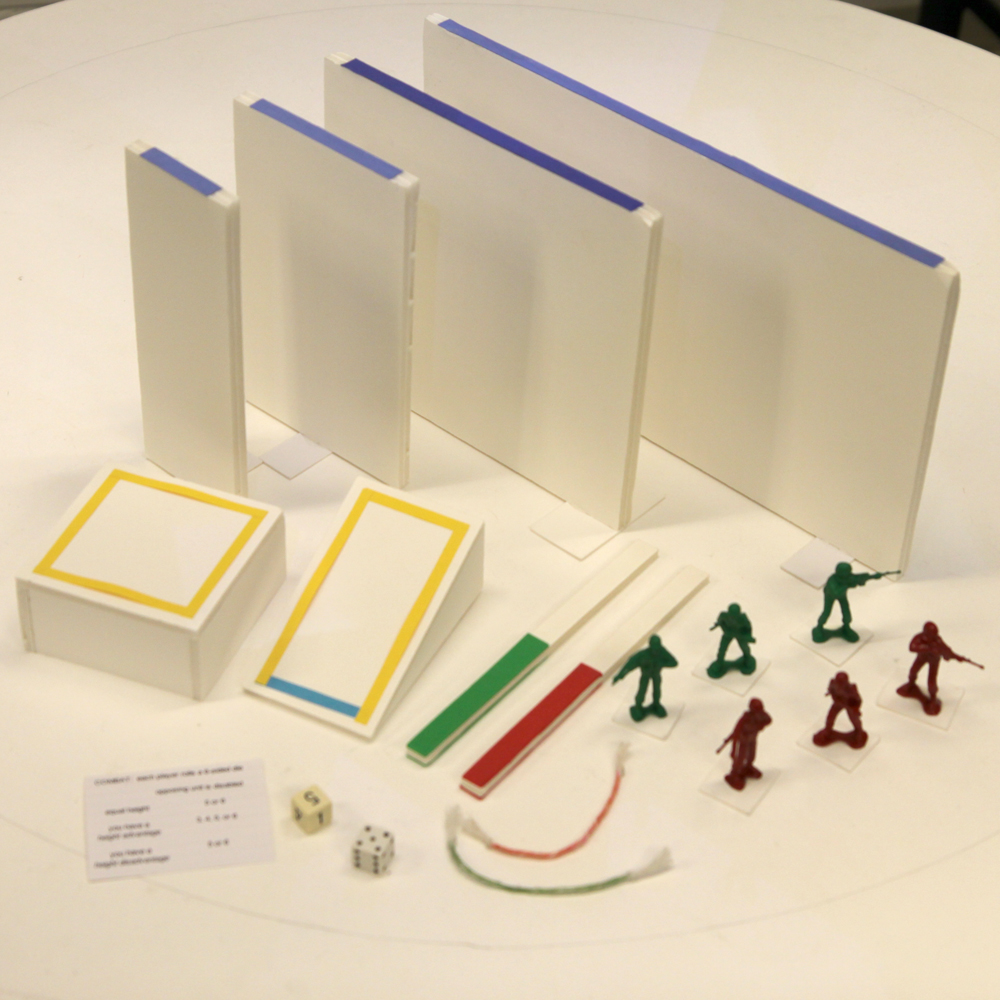
\includegraphics{../gi2012_army/images/props_2.jpg}}
\resizebox{\picwidth}{!}{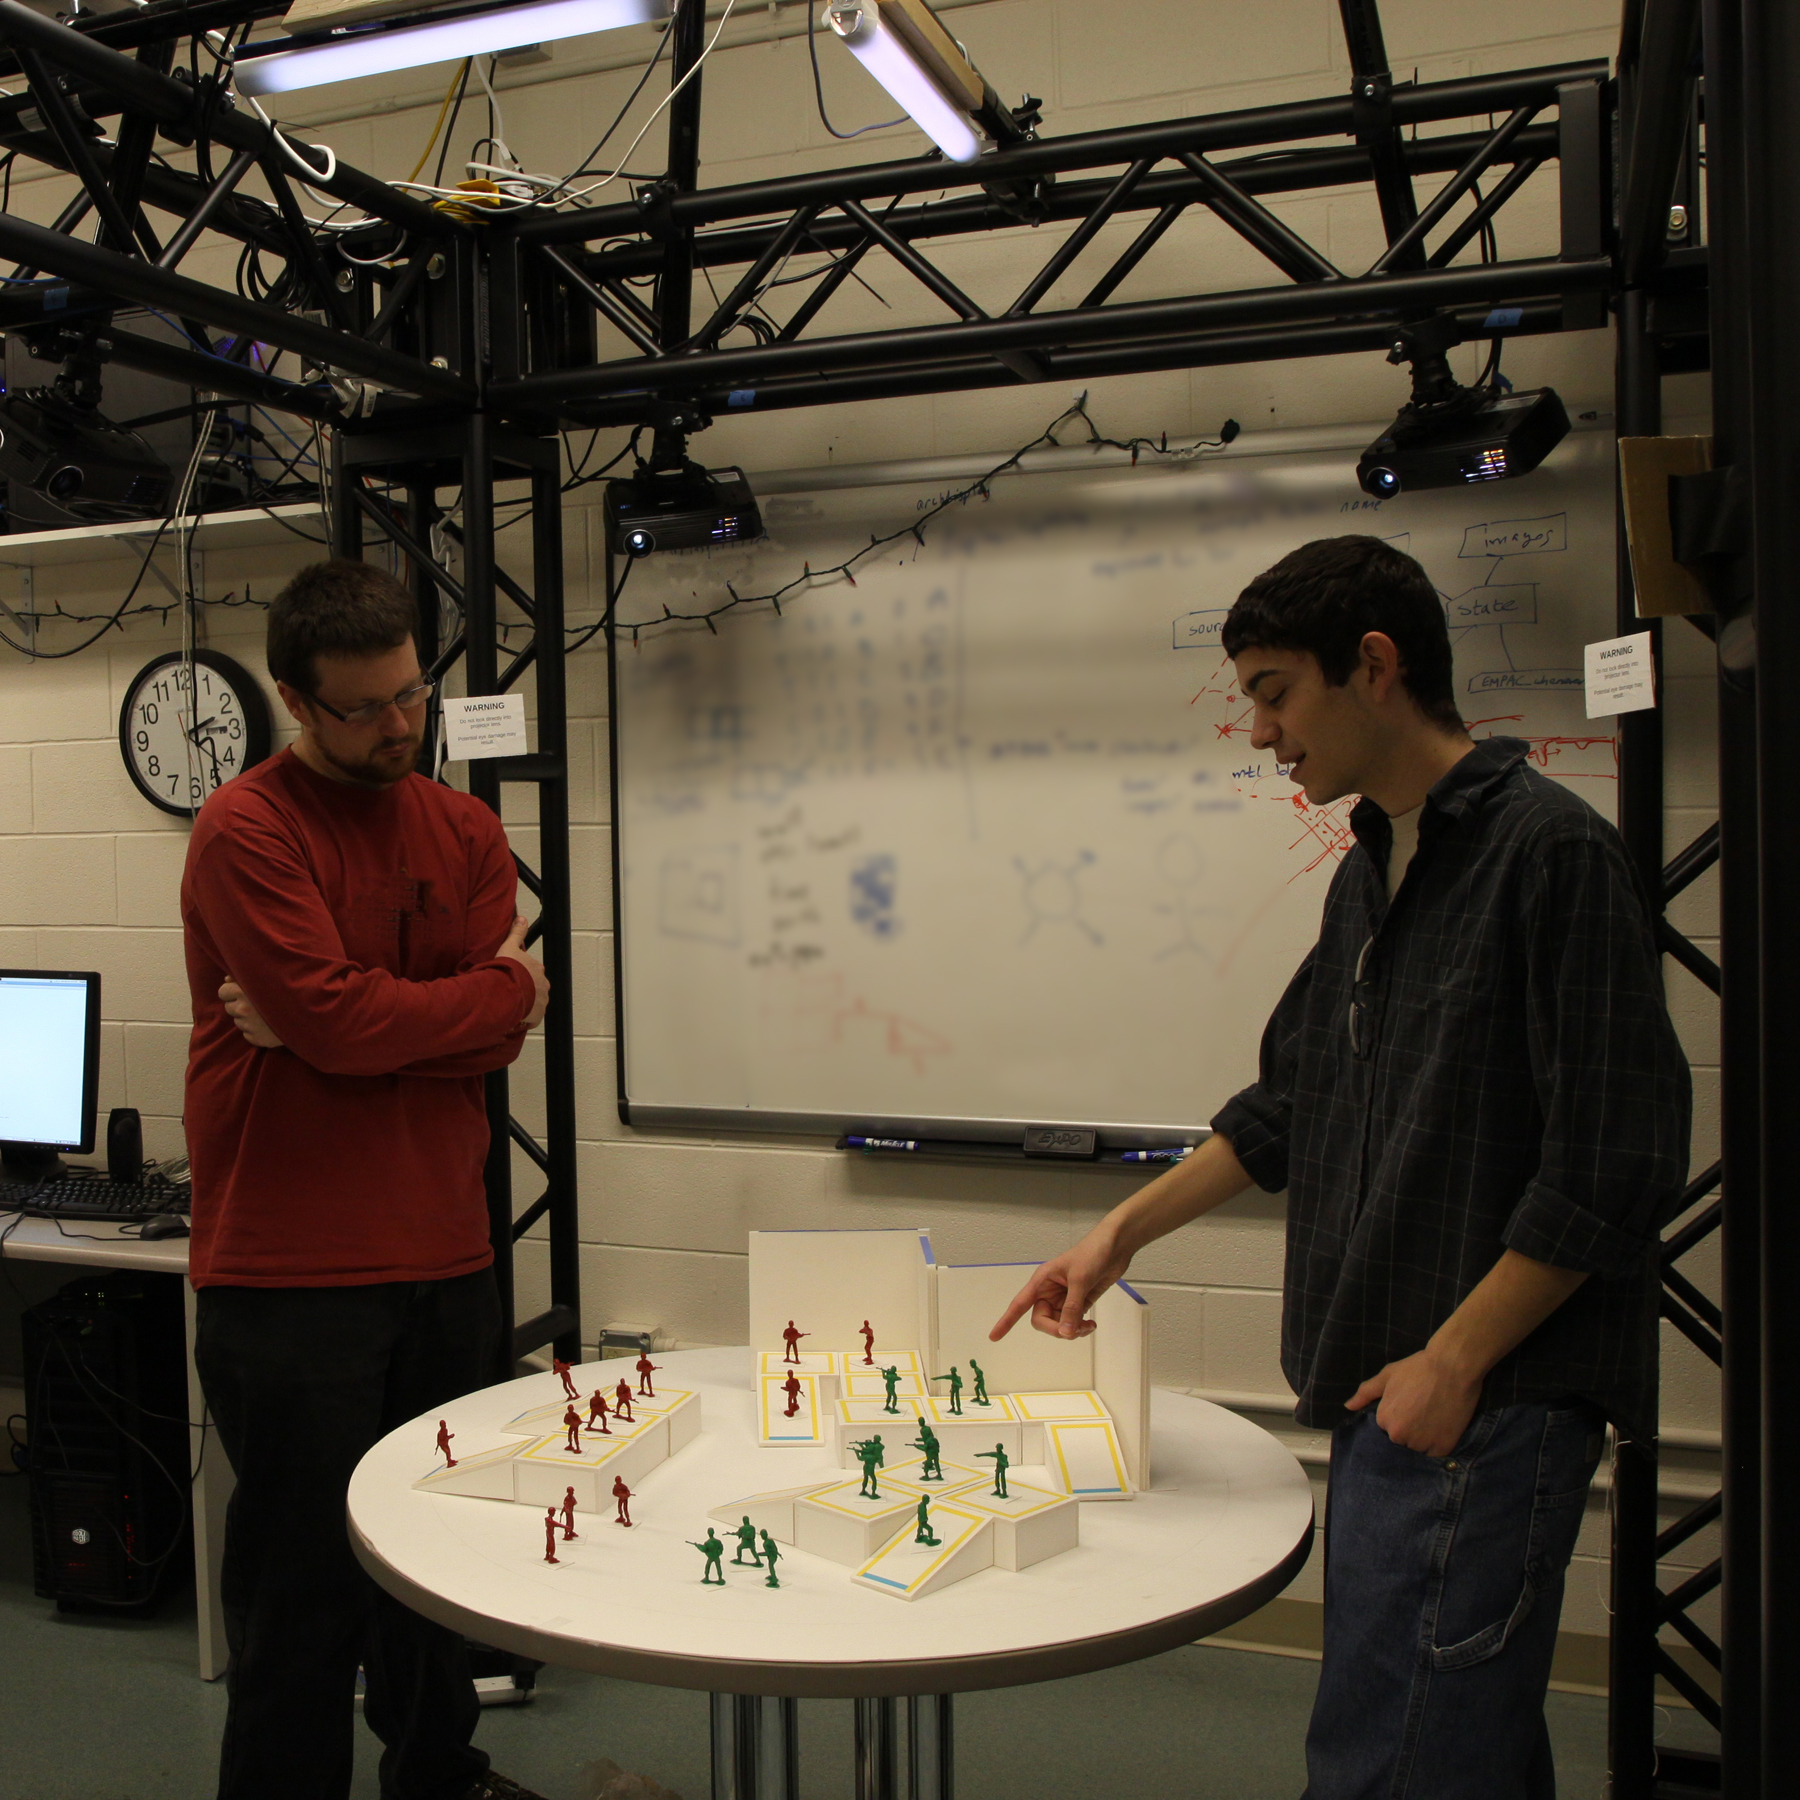
\includegraphics{../gi2012_army/images/contraption_with_people_blur.jpg}}
%\vspace{-0.02in}
\caption{ARmy is played using a set of physical 
%props 
%and a simple
%  wireless remote.  The prop library contains plastic soldier
  soldier figurines and foam-core terrain objects, including walls,
  platforms, and ramps.  The non-augmented version is played with measuring sticks, string, and dice.  
%\fbox{add string, sticks, and dice to left picture}
The SAR version is equipped with a overhead
single camera for object detection and multiple projectors for
display.  
%It is designed to fully cover the surface of a centered
%table, which acts as a space for user interactions.  
}
\vspace{-0.1in}
\label{FIGURE:props_and_contraption}
\end{figure}






\vspace{-0.1in}
\paragraph{Tangible Interaction}

Tangible user interfaces allow interaction and control of the virtual
world by manipulating physical
props~\cite{Fitzmaurice:1995:BLF:223904.223964}. 
% to \fbox{Could mention the bricks paper near here}
Implementation of complex systems with many different types of input
and display devices~\cite{MacWilliams:2003:HSL:946248.946803} allow
users to collaborate in an intuitive manner.  The combined virtual and
physical world even allows remote users to
interact~\cite{Wilson_playtogether:playing} as if they were together
physically.
%
%\emph{Herding Sheep} presents a
%tangible interface that allows interaction in a number of ways
%including a head mounted display, tangible sheep, a laptop and a
%palmtop.  The system includes the 'flocking dynamic' as
%well
%
Tangible environments allow users to designing a custom space and
explore visualizations of the
geometry or run simulations that
interact with the environment~\cite{Ishii:2004:BCS:1031314.1031369,DBLP:conf/ismar/JonesSCGB10}.
%
{\em IncreTable} demonstrates how robots facilitate virtual elements
and simulations impact our physical
spaces~\cite{Leitner:2008:IMR:1501750.1501753}.
%\fbox{paragraph recently added} \emph{IncreTable} provides multimodal
%interaction.  A tabletop system with detectable terrain (using a depth
%camera) allows users to to use both physical objects, including
%dominoes and simple robots, and virtual objects including a virtual
%car and virtual dominoes
%
%: digital clay
%
%\fbox{reword josh add?  let's discuss} Digital design uses user
%defined sand and clay surfaces that can be projected on.    Slope
%variations and curvature, shadows, view-sheds and least cost of
%passage can all be calculated using landscapes created with these
%mediums~\cite{Ishii:2004:BCS:1031314.1031369}.
%
%
%\fbox{josh add ?  lets discuss...}This system can detect complicated surfaces and then
%allow users to manipulate virtual objects on the surfaces using a
%stylus~\cite{DBLP:conf/ismar/JonesSCGB10}.
%

Tangible interfaces can be applied to education, e.g. teaching
billiards~\cite{Suganuma:2008:BIS:1501750.1501752} and games including
%
%examples of other AR GAMES
%
%INTERACTION? People can now play actually board games against someone
%remotely by having the remote persons pieces be projected onto a local
%board.
%
tile-based board games~\cite{Rooke:2010:PDT:1709886.1709932} and
%Even games like Settlers of Catan are being improved using specially
%designed hexagonal pieces
%
robot battle games~\cite{KOJIMA:2006:ACA:1109723.1110608}.
%One more 2D AR game presented has battling
%robots.
%
%
%
%
%Am impressive AR tabletop system that has interactions available with a head mounted display, laptop, palmtop, magic wand, and microphone?  The specific application shown in this paper involves a herd of sheep complete with them using flock behavior.  They also provide a tangible sheep that can be used to steer the behavior of the other sheep.  While they’re system is (more) impressive, our system provides both battle simulation as well as tangible terrain which influences gameplay~\cite{MacWilliams:2003:HSL:946248.946803}.
%
%
%Systems are also being developed as tutorials. One system is designed
%to teach beginners billiards by telling them what the appropriate shot
%is and correcting a users `stance' if it is
%incorrect
%
We have designed the ARmy game to mimic existing board games for
users familiar with these game dynamics.
% they are already familiar with.  
%By allowing users to both have detectable terrain and battle
%simulation we hope to prove the worth of augmented reality battle
%games.\fbox{???}


\begin{figure*}[t]
\begin{center}
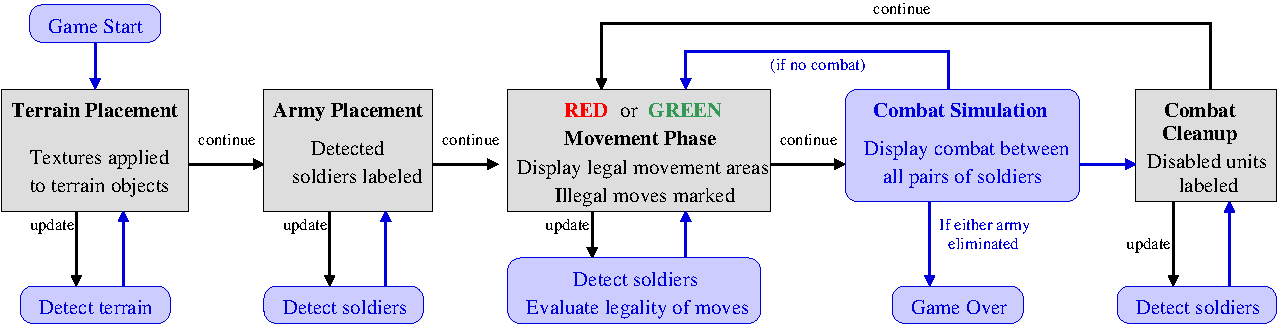
\includegraphics[width=6.5in]{../gi2012_army/images/game_diagram_horizontal.pdf}
\end{center}
\vspace*{-0.05in}
\caption[ARmy Application State Diagram]{State diagram of the
    ARmy application.  Gray boxes represent stages of play defined by
    player actions.  Blue boxes represent stages performed completely
    by the game module.  Similarly, black arrows represent transitions
    triggered by the players via the remote control, while blue arrows
    represent automatic transitions.}
\label{FIGURE:ARmyDiagram}
\vspace{-0.1in}
\end{figure*}



\section{ARmy Game Design}

%\fbox{perhaps summarize contributions of systems before delving into system details?}
%nobody has produced a table-top, multiplayer,
% simulation/strategy/wargame style game (from reviewer)

The ARmy application is a military simulation game played between two
opponents.  Each player controls 
%The players are given a number of 
a set of plastic soldier
figurines, referred to as \emph{units}, which represent their
respective armies (Figure~\ref{FIGURE:props_and_contraption}).  
%hese units 
%Each
On each turn the player moves his units and
%through the scene according to the rules of the
%game, 
engages in combat with opposing units to eliminate them from
play.
%  Victory is achieved by completely eliminating the opposing
%army.
%, or by having the most units at the end of a set time limit.
%
%As with other tabletop games,
% are played over a number of turns consisting of
%multiple steps, through which the players progress at their own pace.
%In the same way, 
%the ARmy application is designed as a series of
%player-controlled feedback loops, meaning that the game module only
%proceeds at the request of the players.  The current implementation
The ARmy game
%application 
is designed as a finite state machine
(Figure~\ref{FIGURE:ARmyDiagram}).  Using a wireless remote control
players send two different signals to the computer game module.
%with a 
%relies on 
%a simple wireless remote control, which allows the players
%to send two different signals to the game module.  
The first is an {\em update request} that tells the game to capture a
new image, detect the current physical game state, and visualize any
new information.
%update its model of the scene and
%display any new information.  
The second is a {\em continue} command indicating that the
players have finished with the current stage of play and wish to
proceed to the next step.  
%Figure~\ref{FIGURE:ARmyDiagram} diagrams
%the overall design of the interaction using a finite state
%representation.



%In designing this application, special consideration was given as to %how SAR techniques could be leveraged to improve upon the play style %of traditional tabletop games.  This section provides a step-by-step %description of how the game is played, as well as how it incorporates %virtual elements to create a new and interesting game experience.





\vspace{-0.15in}
\paragraph{Terrain Placement}


%% %FIGURE : TERRAIN DETECTION IMAGES
\begin{figure}[b]
\vspace{-0.08in}
\newcommand{\picwidth}{1.625in}
 \resizebox{\picwidth}{!}{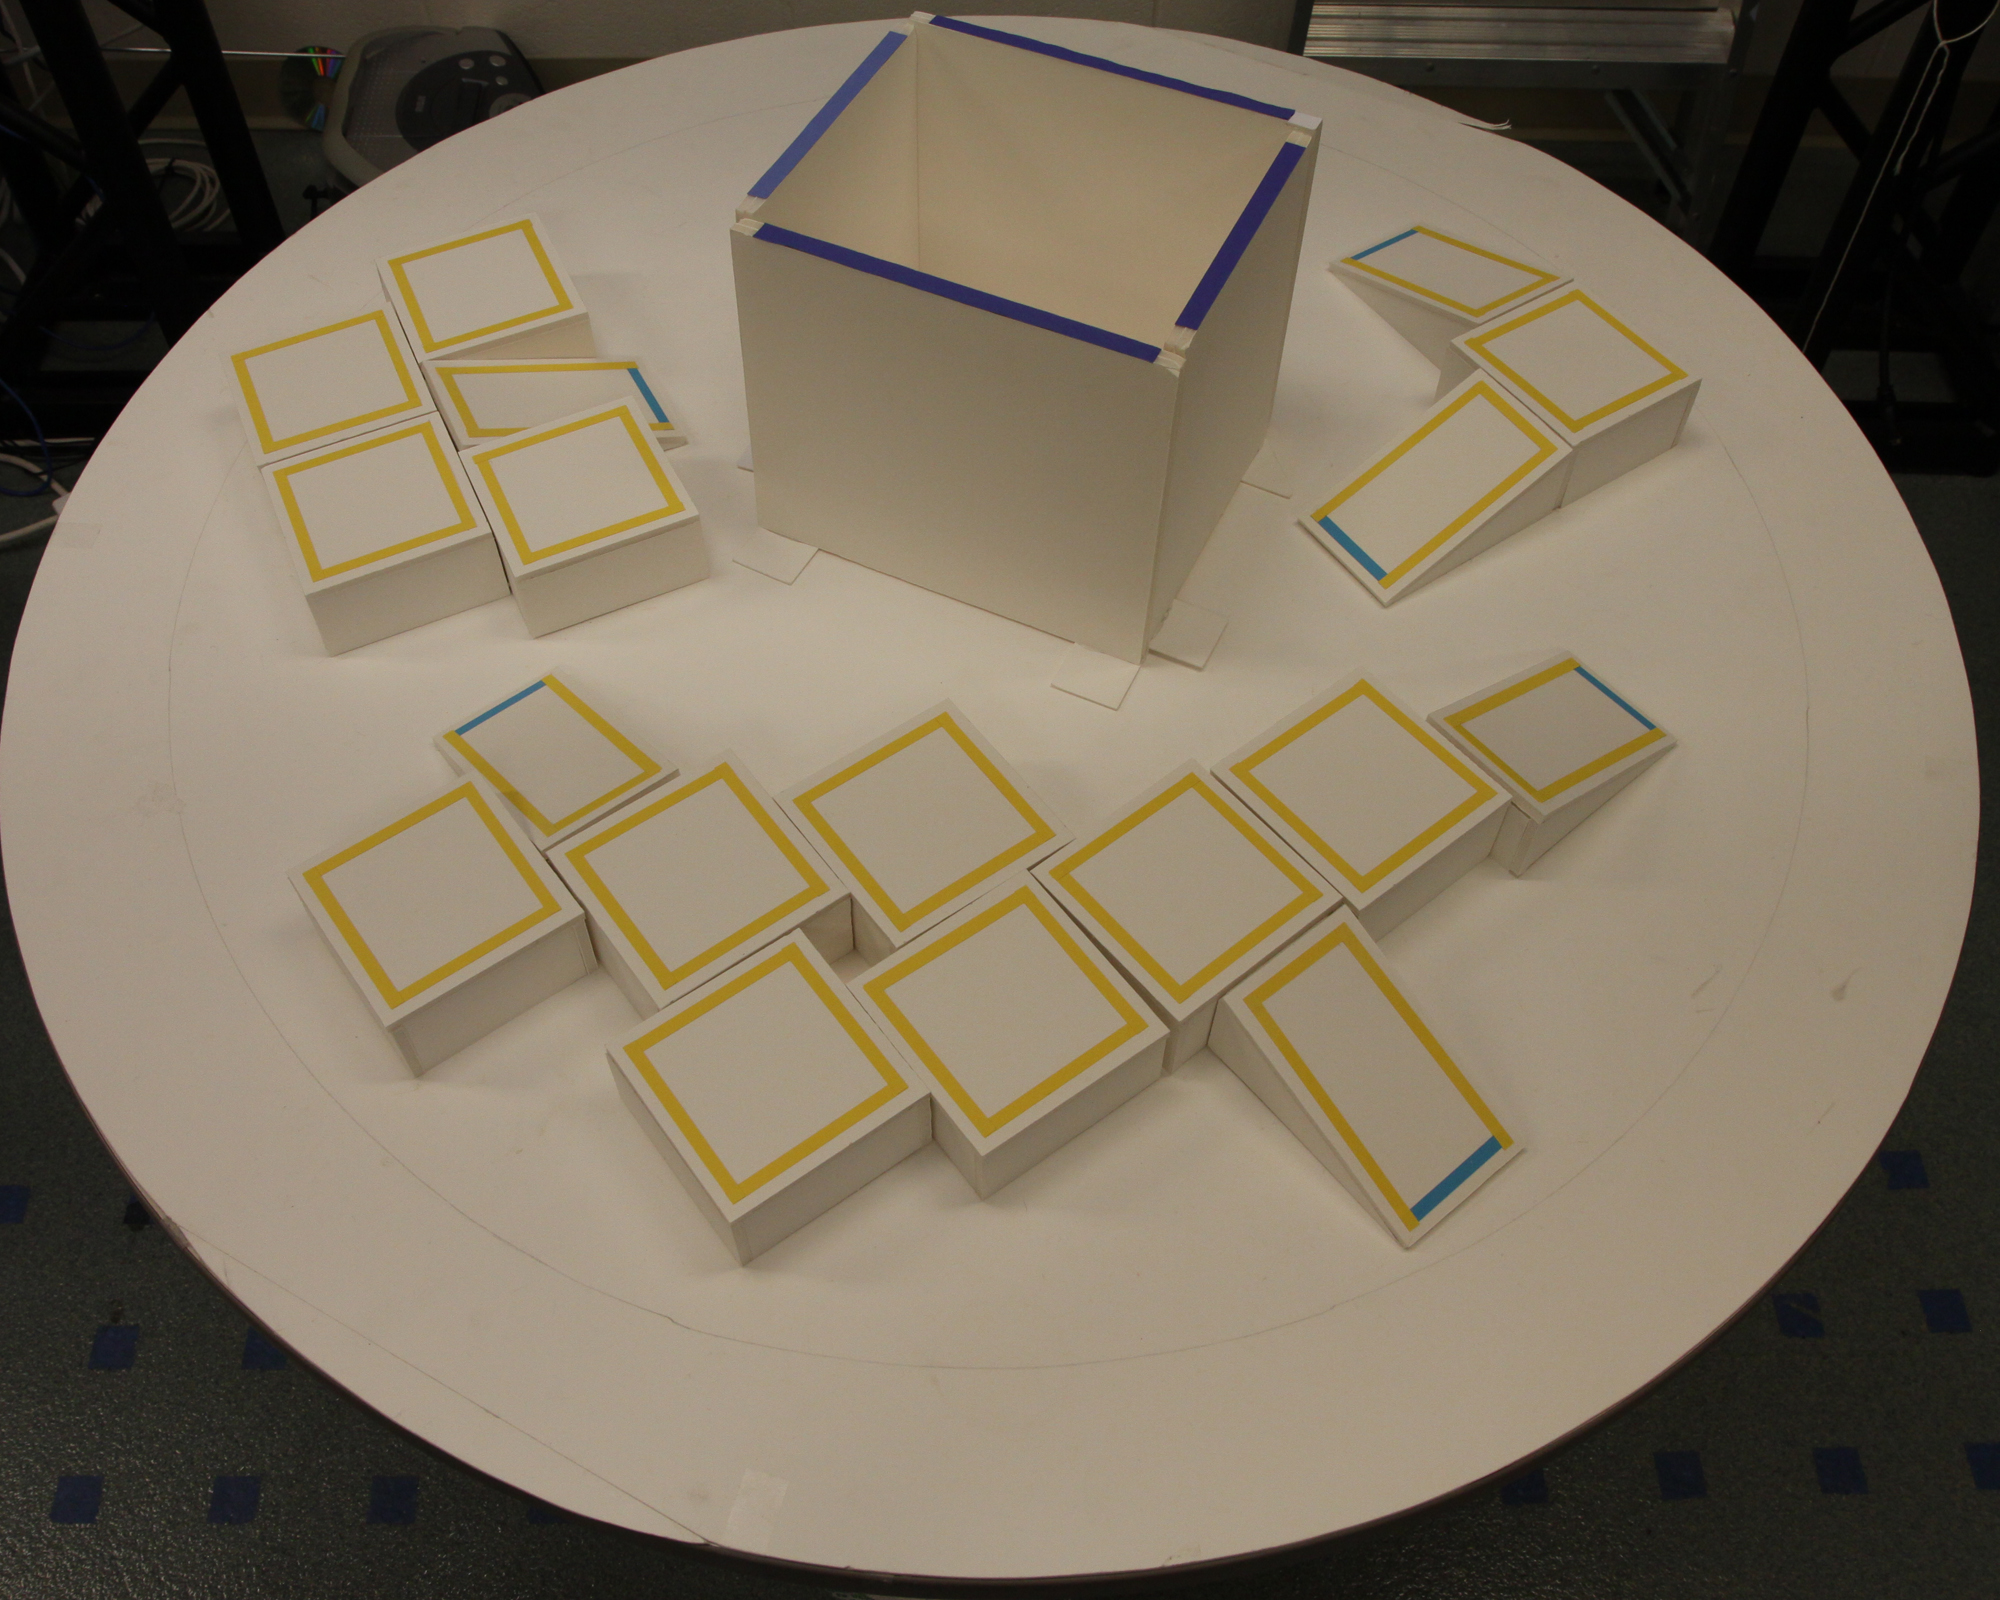
\includegraphics{../gi2012_army/images/complex_lights_on.jpg}}
 \resizebox{\picwidth}{!}{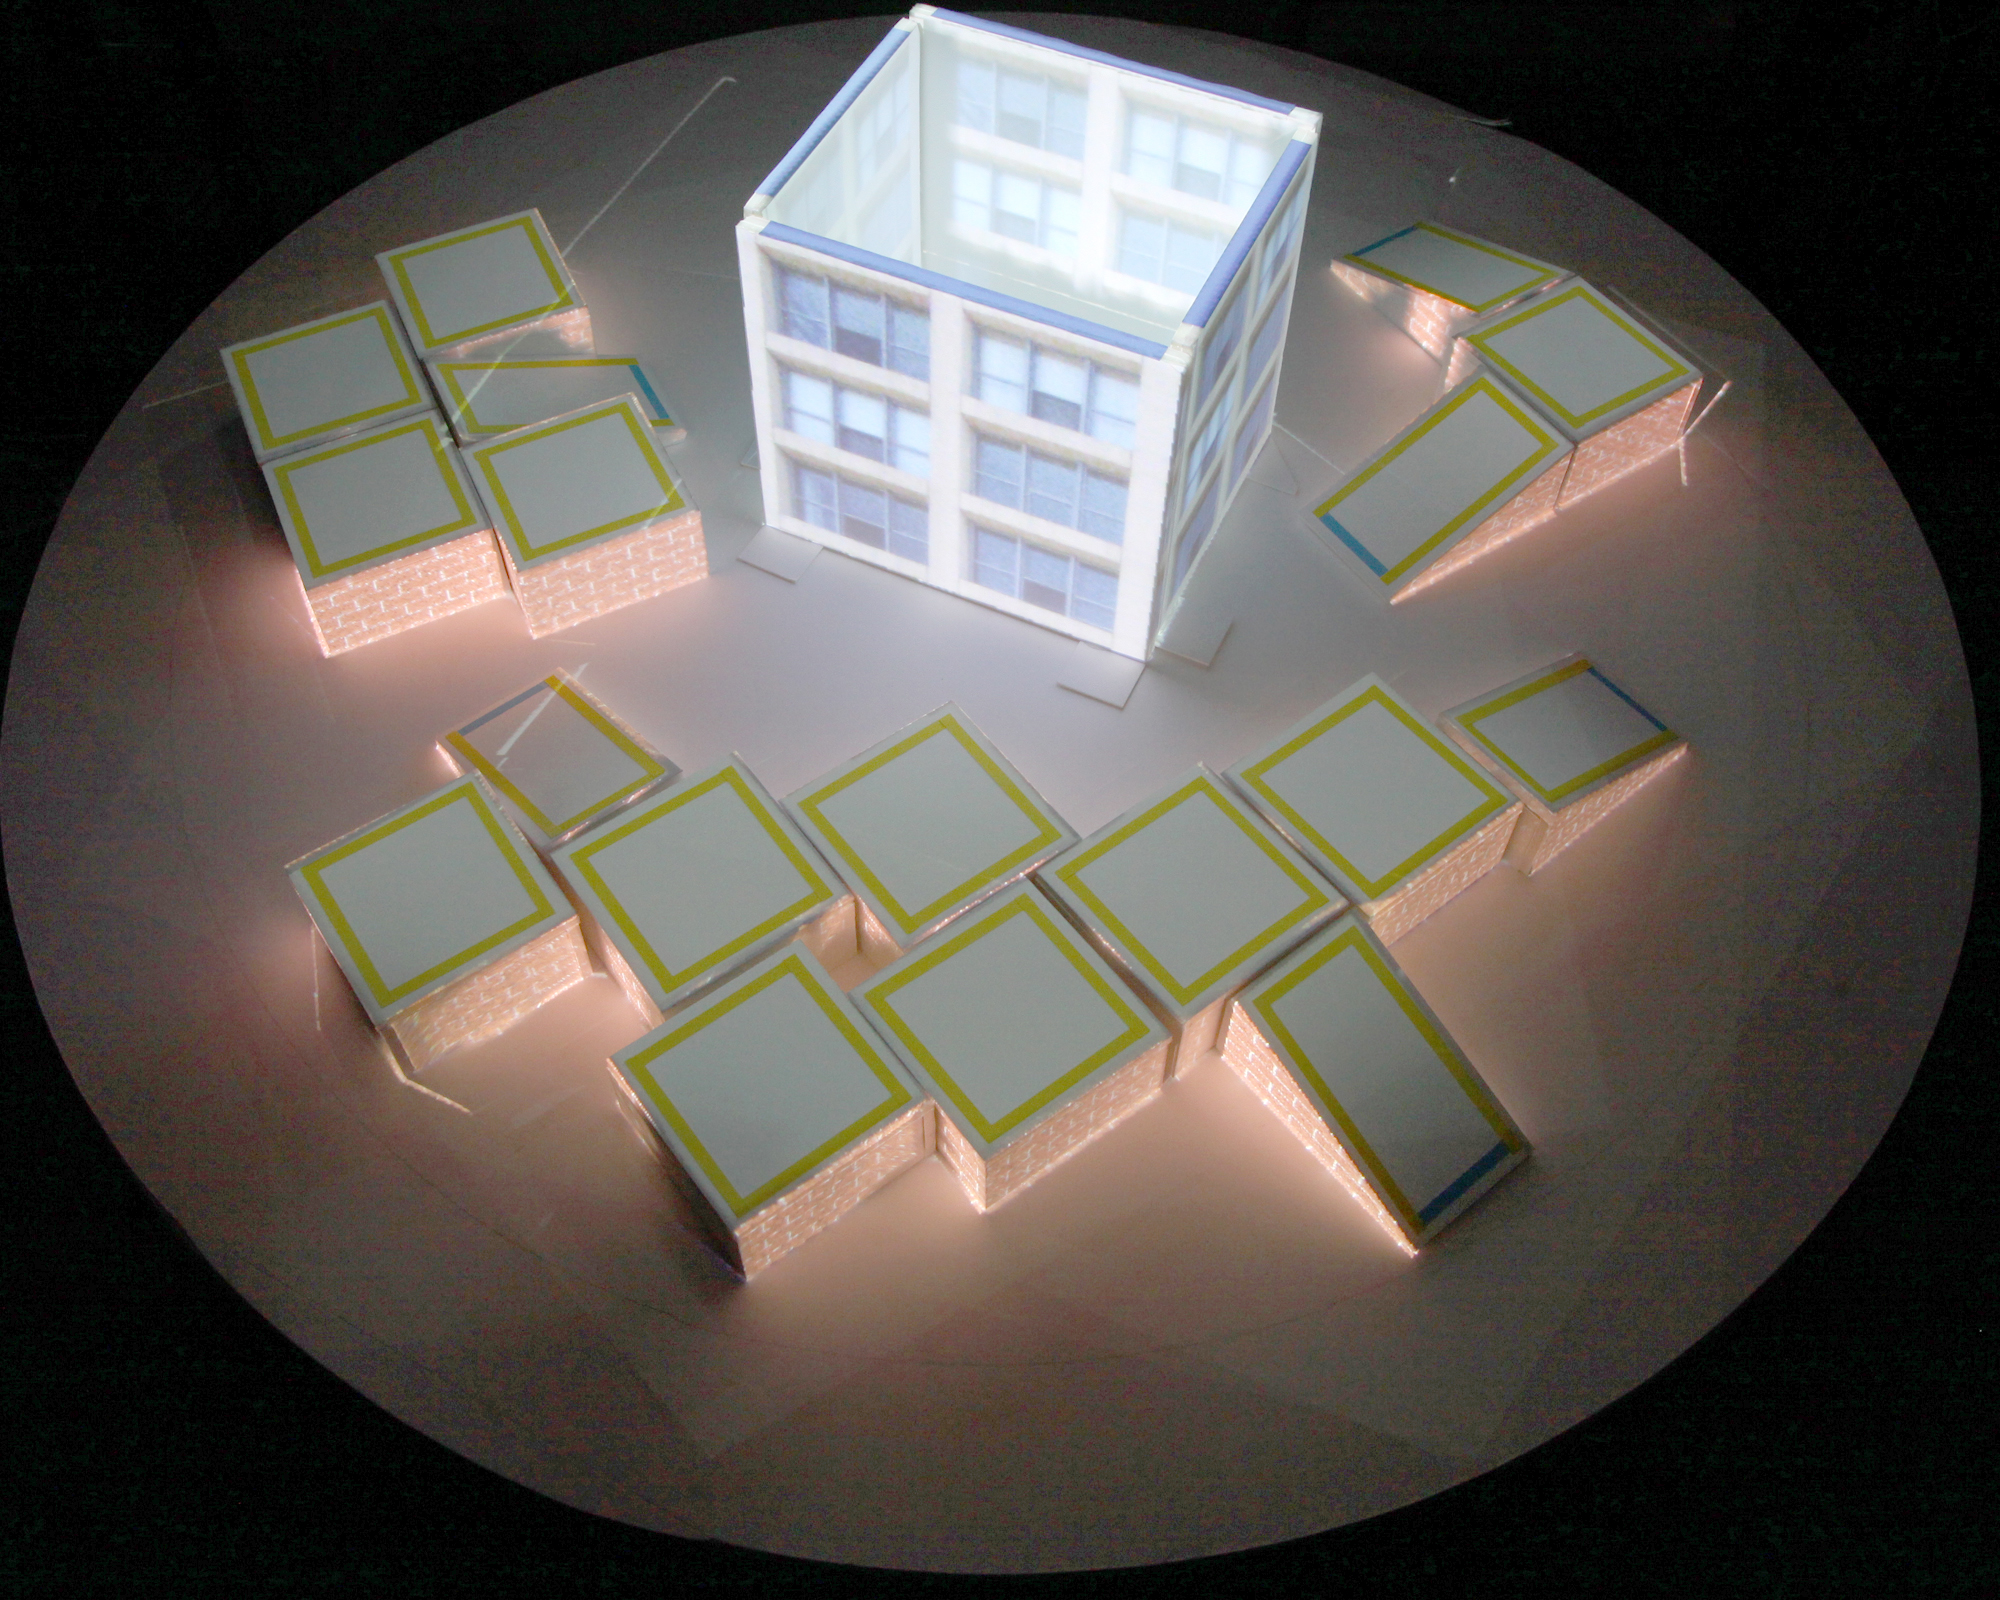
\includegraphics{../gi2012_army/images/complex_projection_lightened.jpg}}%
%\vspace{-0.1in}
\caption[Terrain Placement]{Players freely arrange platform, ramp, and
  wall terrain objects in the scene, and our system detects and
  augments these objects with appropriate and interesting textures. }
\label{FIGURE:TerrainPlacement}
\vspace{-0.08in}
\end{figure}


%% An important aspect of many tabletop games, particularly those that %% involve military strategy, is the idea that the game world is not flat %% and uniform, but rather that it is characterized by varying terrain.  %% As in the real world, terrain represents variations in elevation and %% environment that affect units within the area.  For example, one kind %% of terrain might represent a swamp that is difficult to walk through, %% resulting in a movement penalty to units attempting to move through %% the terrain.  Another might represent tall grass that provides some %% degree of cover, thus making it more difficult to fire at concealed %% units in combat.  

%Walls represent tall barriers through which units cannot move or see.  %Elevated platforms serve a similar function, but differ in that units %may stand and move around on top of them.  

%Like most miniature war games, 
ARmy is played on a varied 3D terrain
surface requiring strategic decision making. The ARmy prototype
provides three simple terrain object types: 8'' vertical walls,
elevated platforms (4''x4''x2''), and ramps (3''x5''x2'').
Units are not allowed to ``jump'' or ``climb'' from low elevation to
high elevation or vice versa, but must instead use connected ramps
to walk between the two.  Controlling elevated terrain and
ramps is important to the strategy of the game, as units that hold the
higher ground receive a significant advantage in combat.
%
%An appealing aspect of ARmy is that, like most miniature war games, %it allows players to be creative in their construction of the game %world, designing the terrain configuration to suit strategies that %seem fun and exciting.  
%% Figure~\ref{FIGURE:GamePrimitives} shows a representative set of %% object types that are used in the game.  Wall primitives are 8'' tall %% by \begin{math}\frac{1}{2}\end{math}'' thick, and are available in a %% variety of lengths.  Elevated terrain is composed of 4'' long by 4'' %% wide by 2'' tall platform primitives, as well as 5'' long by 3'' wide %% ramp primitives.
%
The game begins with a \emph{terrain placement} step, during which
players collaboratively construct the terrain by freely placing
provided terrain primitives on the table.
%(Figure~\ref{FIGURE:TerrainPlacement}).  
Each primitive is constructed
from diffuse white foam-core with simple unobtrusive colored markings
to facilitate detection.
%To simplify the game rules as well as the
%task of detecting the terrain, 
%We require that platforms and ramps
%will not be stacked on top of each other, and that terrain placement
%will not change after the game has begun.  
%After both players have
%agreed upon an acceptable terrain configuration, they 
%signal the application, which locks their decision.
%
%% In traditional miniature war games, players are typically allowed to %% represent terrain using whatever objects or methods may be available %% to them.  However, many players prefer to use objects that physically %% resemble the terrain that they represent in order to make it easier %% for players to remember the meaning of each object.  In addition, %% realistic terrain objects help to create a more aesthetically sound %% environment, which may help some players to feel immersed in the %% miniature world of the game.  In this regard, techniques for spatial %% augmentation hold great promise as a means of flexibly applying a wide %% number of aesthetic choices to a single primitive object.
%
The ARmy application uses SAR projection
%the underlying SAR projection system 
to apply virtual textures directly onto the physical terrain
primitives (Figure~\ref{FIGURE:TerrainPlacement}).
% shows an example
%terrain configuration with and without augmentation.  
%Brick textures are applied to the sides of elevated ramp and platform
%terrain, and a windowed building facade texture is applied to the wall
%surfaces.
%.  Of
%course, these textures are merely an example of one possible aesthetic
%choice, and could easily be replaced with anything desired by the
%players, such as grass, concrete, or sandbags.

%% It is important to note that many players of miniature war games enjoy %% constructing and customizing terrain objects as much as they enjoy %% playing the game itself.  For this reason, an ideal application of %% spatially augmented reality would not prohibit players from crafting %% and using such objects.  In other words, visual augmentation is not %% intended to replace fine craftsmanship, but instead to be available %% only when players desire it.  For example, consider a situation in %% which a player wishes to make last-minute changes to a setup, thus %% requiring him to add primitive objects to an otherwise highly-detailed %% scene.  In this case, projecting a few well-chosen textures can help %% maintain the visual integrity of the game.

\vspace{-0.15in}
\paragraph{Army Placement}

%After configuring the terrain, 
Next, players 
%decide on rules for 
position
their respective units (following mutually agreed upon rules), 
%ies.  Units are 
represented by 2'' tall red or green plastic
soldier figurines.
%, which have been colored with red or green spray
%paint to denote player ownership.  As in any figurine-based tabletop
%game, 
%Units are positioned by physically placing them on the table.
%At any point during this step, 
Players may request an update from the game module, which will then
detect all positioned figurines, marking each 
with a 
%colorful
projected icon to show that it has been successfully recognized.
%, as depicted in
%Figure~\ref{FIGURE:CombatMovementExample}b.  
When all units have been placed to the players' satisfaction, they
signal for the game to start.



% FIGURE OF EXAMPLE MOVEMENT REGIONS
\begin{figure}[b]
\vspace{-0.08in}
\newcommand{\picwidth}{1.625in}
\resizebox{\picwidth}{!}{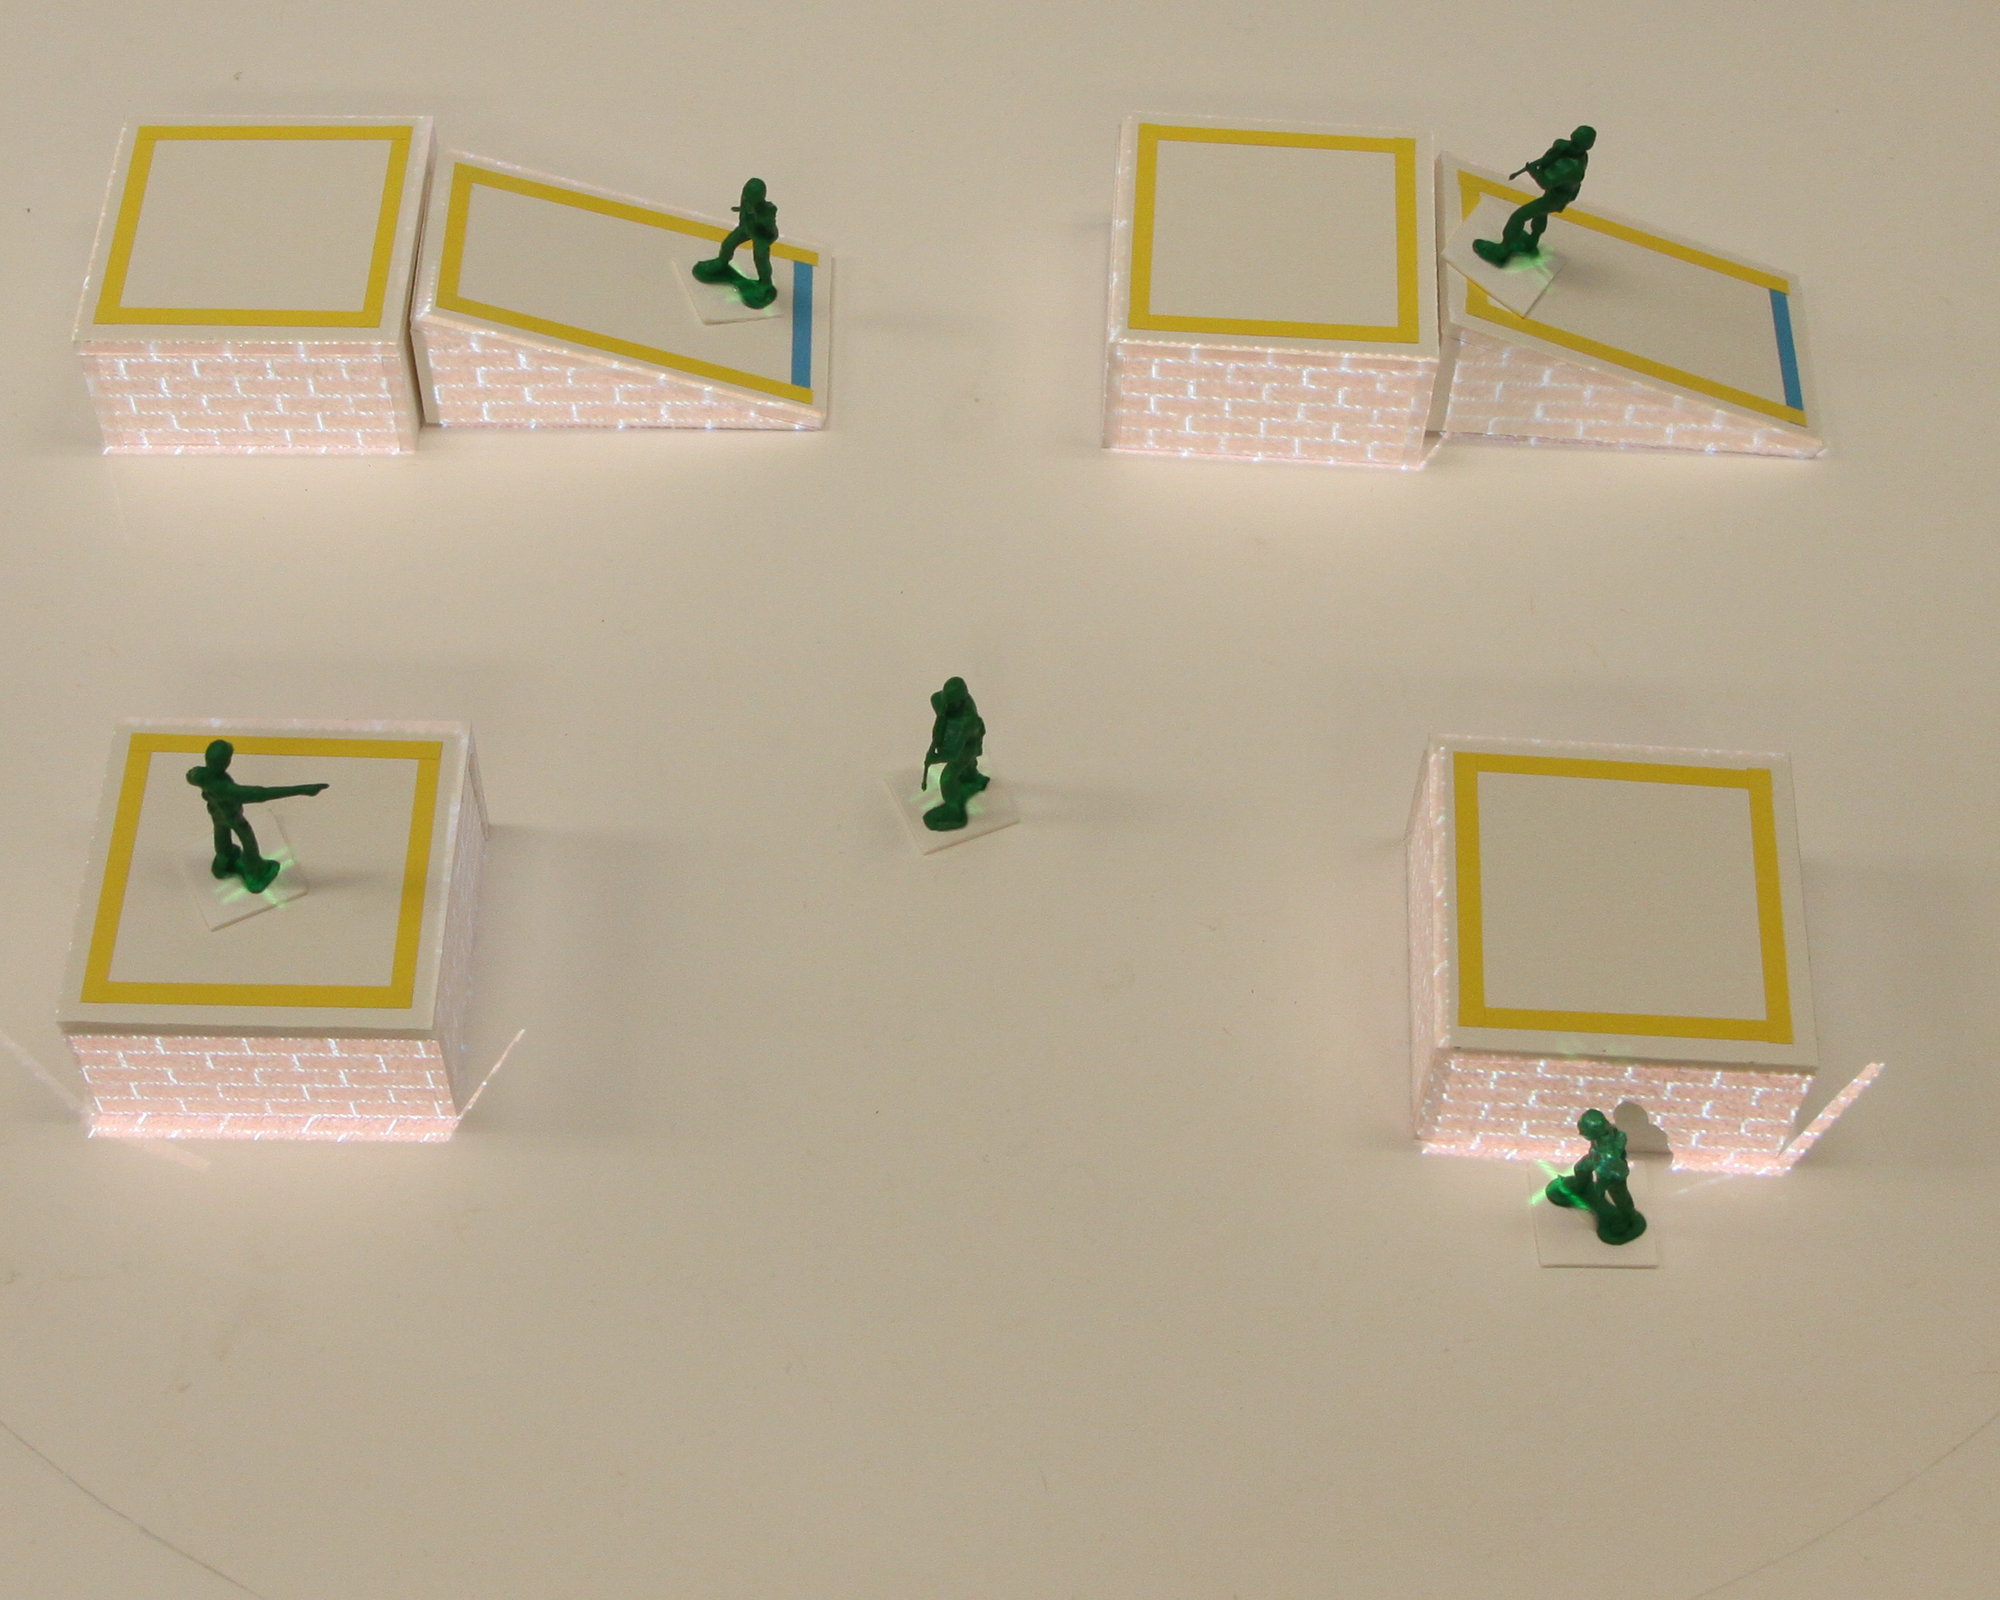
\includegraphics{../gi2012_army/images/movement_terrain_projection_lights_on_with_army.jpg}}
\resizebox{\picwidth}{!}{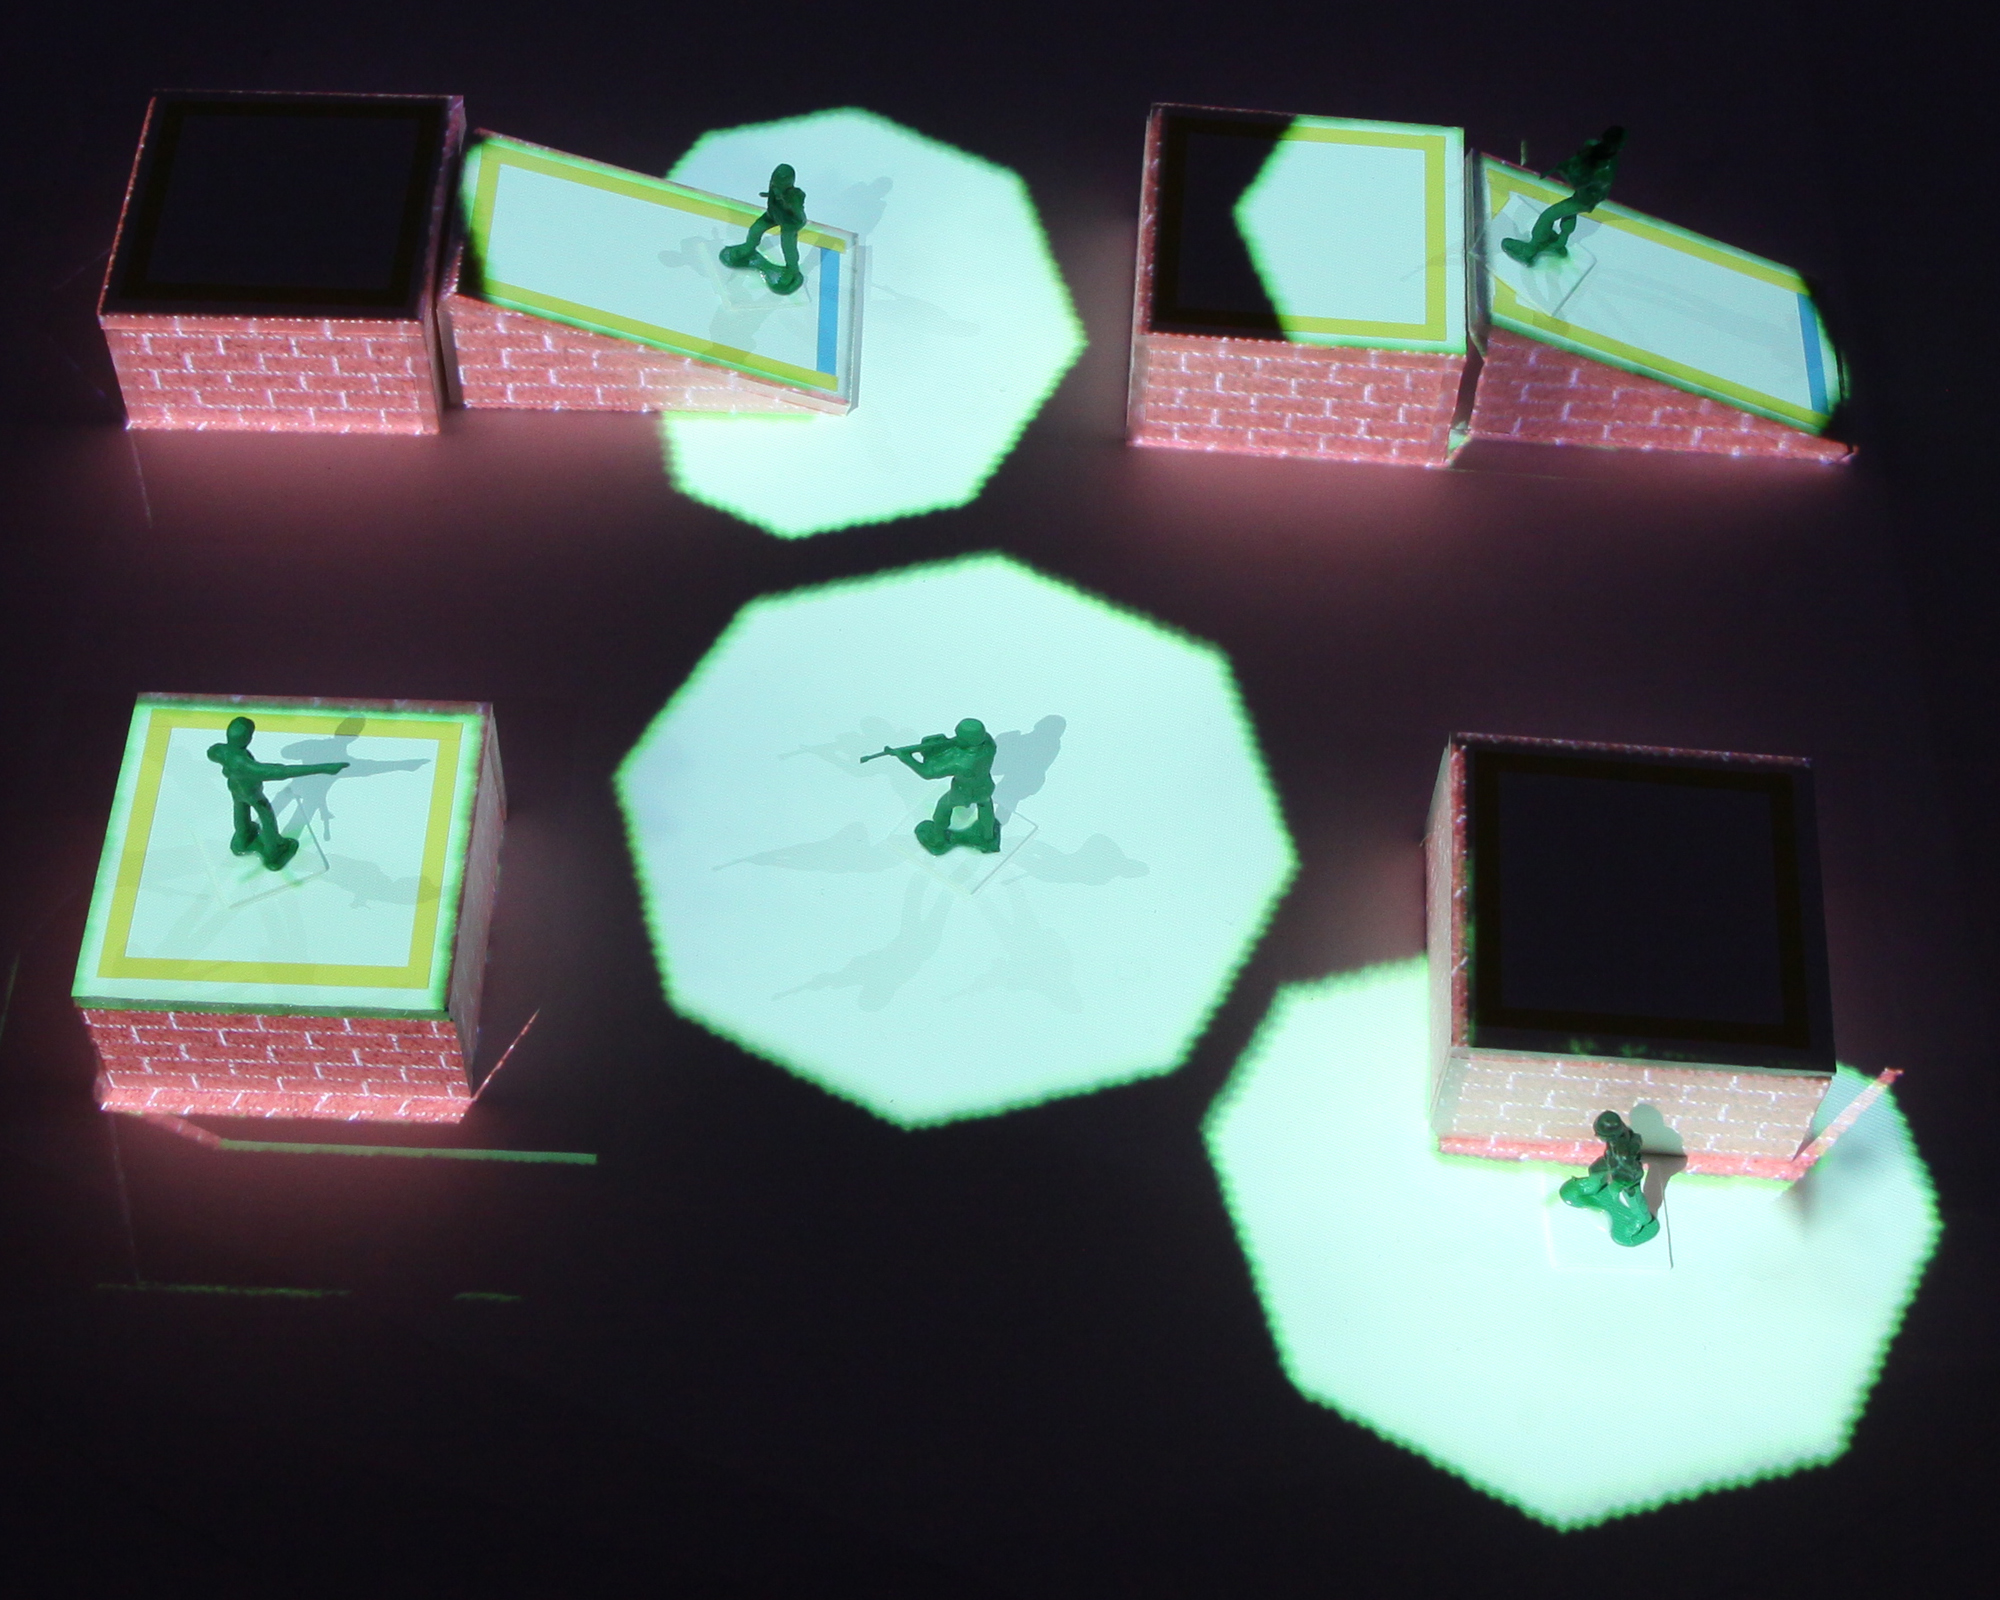
\includegraphics{../gi2012_army/images/movement_circles_projection.jpg}}%
\caption{During the \emph{movement phase,} each unit's field of
  movement 
%(limited to 4'') 
is illuminated.  Note that the visualization conforms to movement rules across terrain
  boundaries, which require the use of ramp objects in order to climb
  up or down elevated platform.  }
\label{FIGURE:MovementRegions}
\vspace{-0.1in}
\end{figure}


\begin{figure*}[t]
\newcommand{\picwidth}{1.12in}
\resizebox{\picwidth}{!}{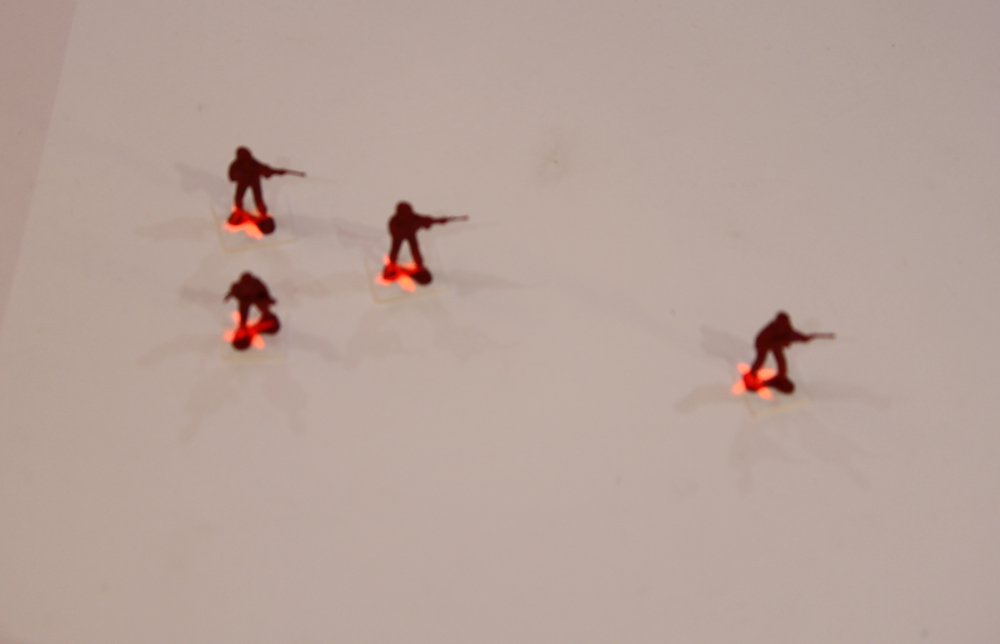
\includegraphics{../gi2012_army/images/movement_0.jpg}}
\resizebox{\picwidth}{!}{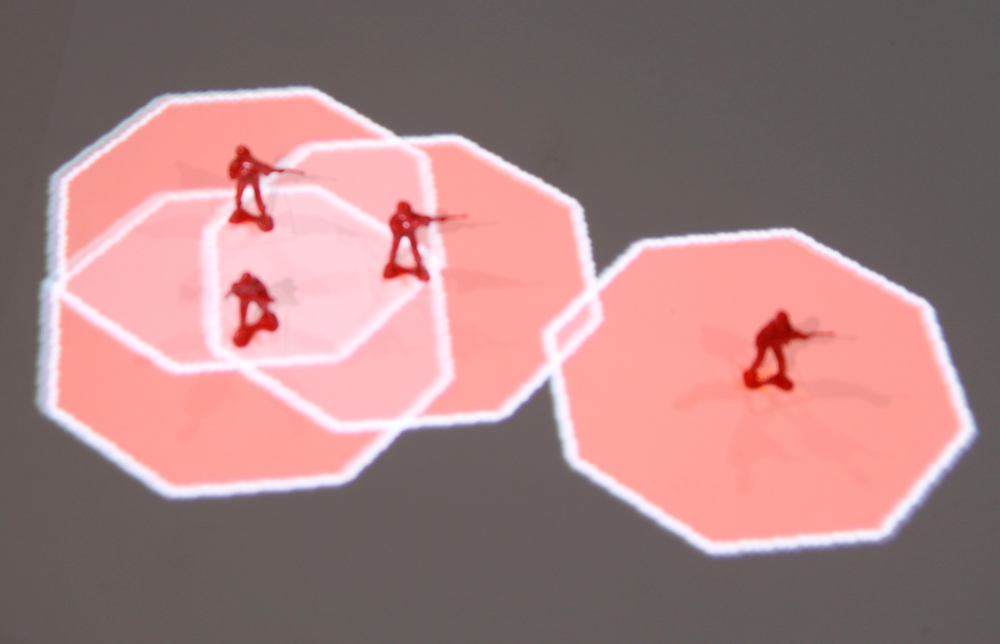
\includegraphics{../gi2012_army/images/movement_1.jpg}}
\resizebox{\picwidth}{!}{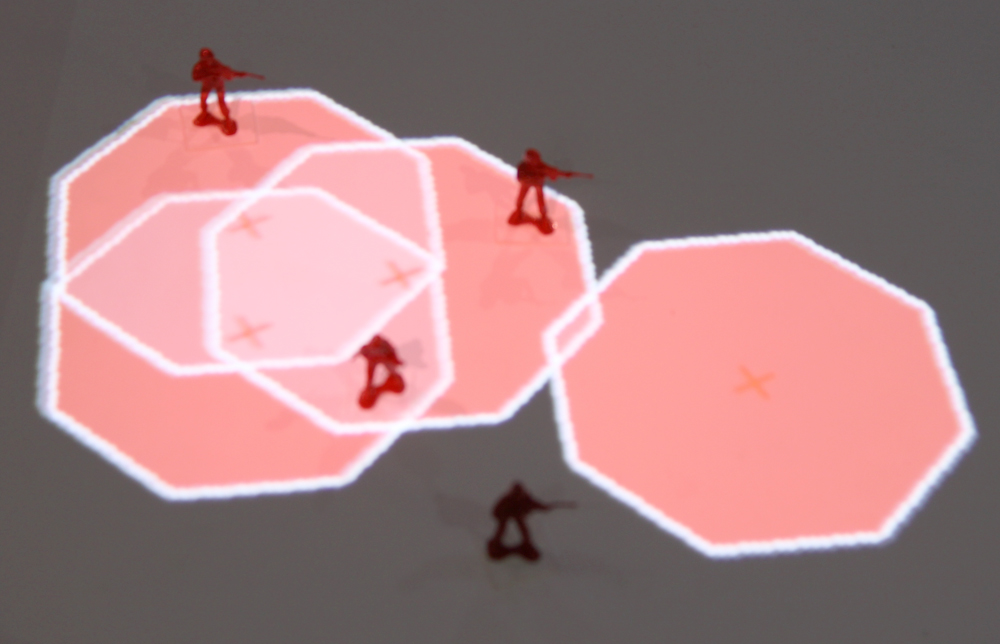
\includegraphics{../gi2012_army/images/movement_2.jpg}}
\resizebox{\picwidth}{!}{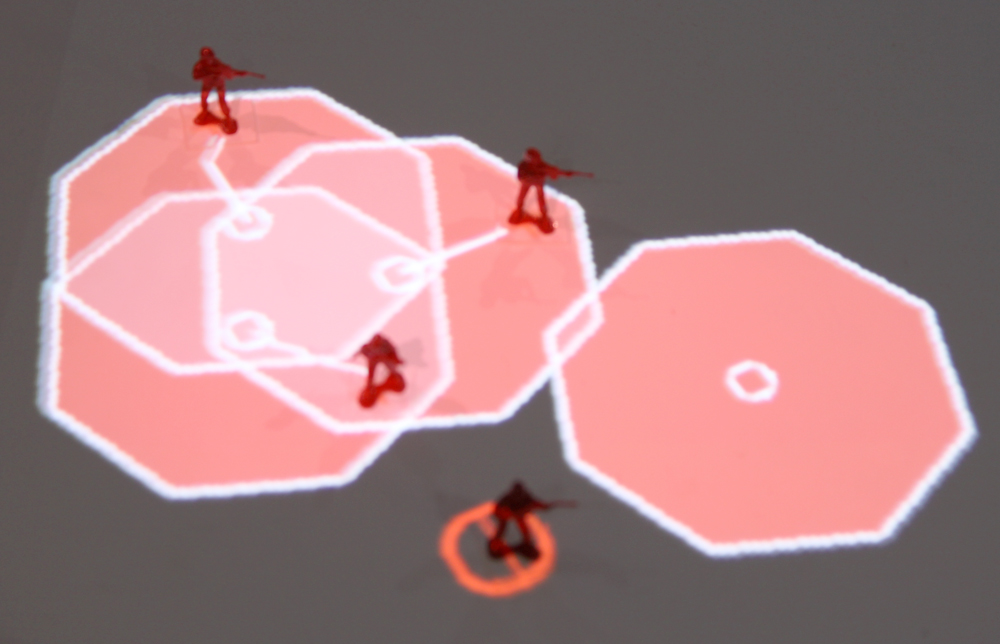
\includegraphics{../gi2012_army/images/movement_3.jpg}}
\resizebox{\picwidth}{!}{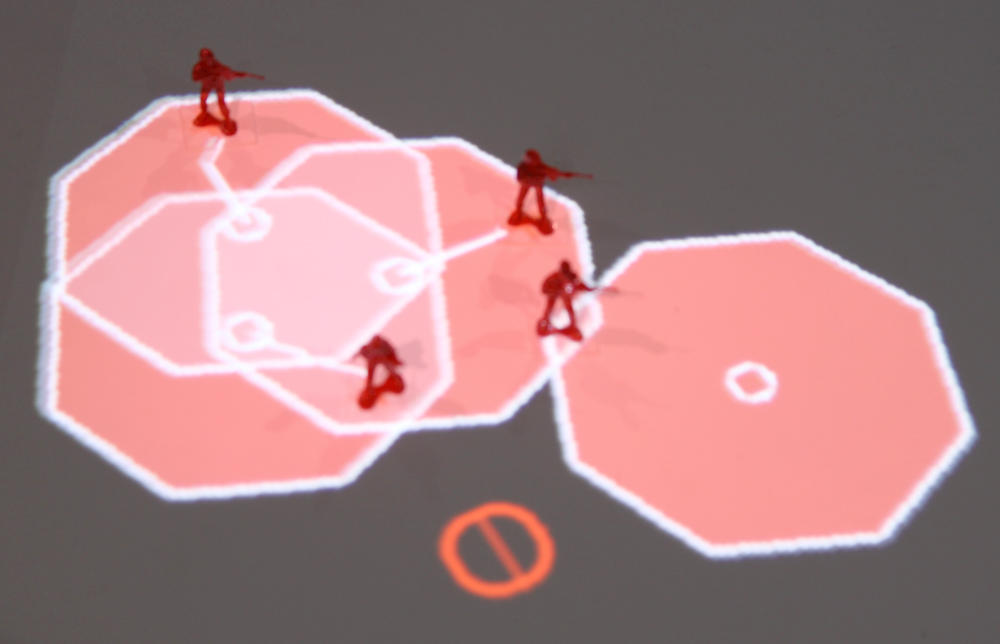
\includegraphics{../gi2012_army/images/movement_4.jpg}}
\resizebox{\picwidth}{!}{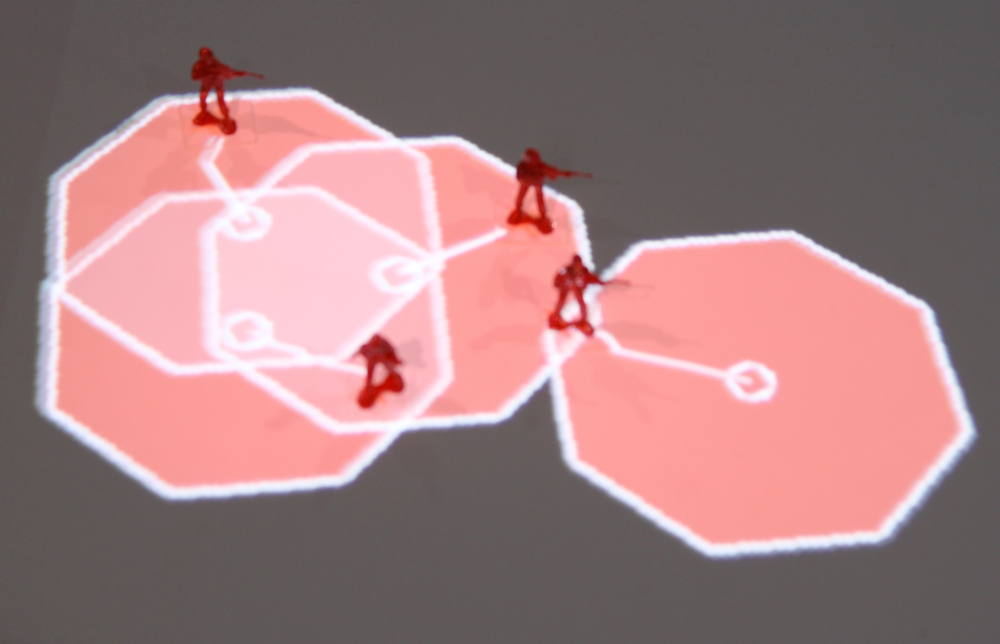
\includegraphics{../gi2012_army/images/movement_5.jpg}}%
%\vspace{-0.1in}
\caption{During each movement phase the player may move all of their
  units simultaneously.  The system matches each unit's current
  position (marked with a ``$\times$'' icon) to its previous position
  (marked with a ``$\circ$'' icon) using the Hungarian Method (drawn
  as a white path).  If no legal move is found the unit is marked
  appropriately with a ``not'' symbol.  The player must then correct the
  error before proceeding.  }
\vspace{-0.15in}
\label{FIGURE:MovementSequence}
\end{figure*}



\vspace{-0.15in}
\paragraph{Movement Phase}

At the start of a player's movement phase, each of his unit's field of
movement is overlaid on the terrain as a colored region
(Figure~\ref{FIGURE:MovementRegions}).  Each unit's movement is
constrained to a maximum distance of 4'' and must conform to the
terrain rules described earlier.  The player may move any number of
his units, and each unit may move anywhere within its corresponding
highlighted region.
%
At any point,
%during the movement phase
the player may request an update of the
visualization from the game module, which will then augment the
overlaid display with a visualization of the detected movements
(Figure~\ref{FIGURE:MovementSequence}).
%Each unit's position at the start of the movement phase is denoted by
%a ``$\circ$'' icon and its current position is marked with an an
%``$\times$'' icon with a white line connecting the positions, marking
%the unit's movement path 
In the event that a given move is invalid, this information is
reflected in the overlay, allowing the player to correct the error.
%The game continues to display the movement zones of each unit from its
%original position, in case the player changes his mind and would like
%to choose a different move for a particular unit.

%Each player's turn consists of a \emph{movement phase}, during which
%he has the option of moving any number of his units.  %As in most
%tabletop war games, 

%
In the %traditional, 
non-augmented version of this type of  game,
%er, a crucial difference is that in a traditional game, 
players measure distances using a ruler or measuring tape.
% to make sure that all moves fall within the acceptable range.  
%
%As
%previously stated, 
Augmentation is helpful
%one goal of augmenting physical games with elements
%of video games is to
in automating tedious tasks
% that would otherwise burden the player, as
and moderating subjective calls that could lead to disagreements
between players about the legality of specific moves.  In the
augmented version,
% of the game,
%In this case, the game module completely eliminates the
the system 
%need for players to manually measure distances by 
clearly and precisely indicates each unit's field of movement, and
marks illegal moves.
%reduces ambiguity in rules by notifying players when a move is
%illegal.  
Additionally, 
%since players may move many units at once, 
the system tracks and displays each unit's original position,
%  which units have already been moved from
%their initial positions, 
thereby avoiding a potential source of
confusion for complex multi-unit battle scenarios.




\vspace{-0.17in}
\paragraph{Combat Simulation}


\begin{figure}[b]
\vspace{-0.05in}
\newcommand{\picwidth}{1.625in}
\resizebox{\picwidth}{!}{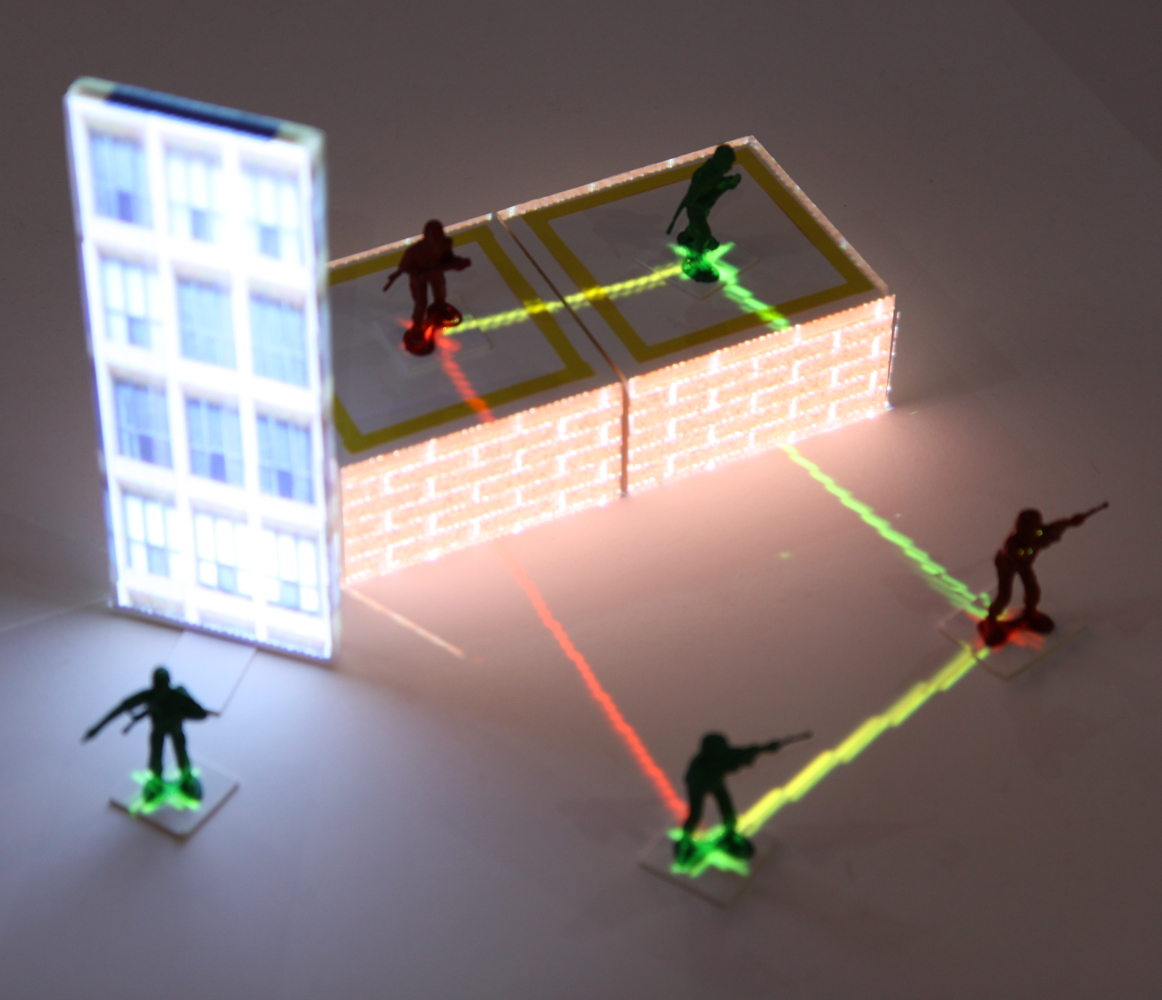
\includegraphics{../gi2012_army/images/combat_image_b.jpg}}
\resizebox{\picwidth}{!}{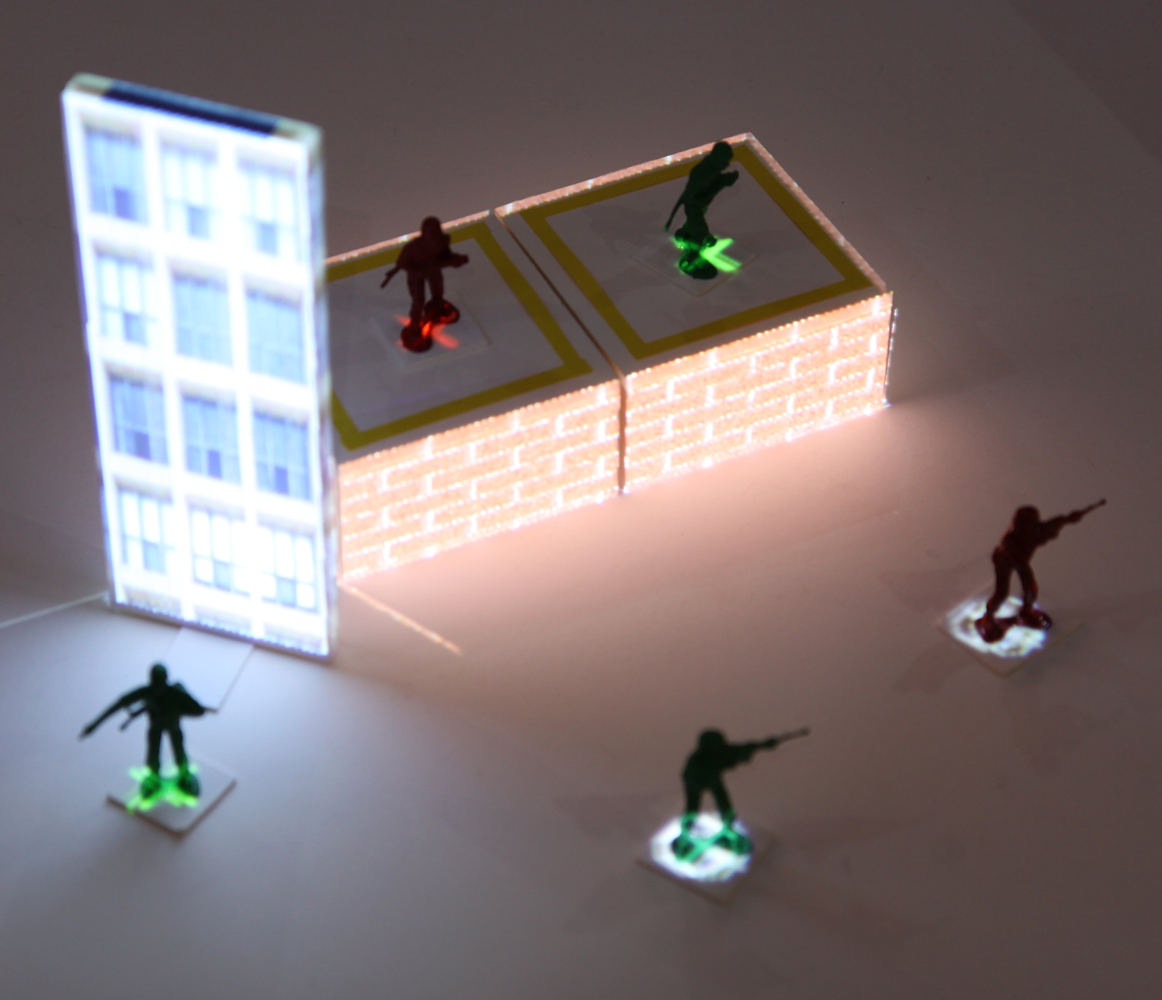
\includegraphics{../gi2012_army/images/combat_image_c.jpg}}%
\caption{Brightly colored {\em combat lines} indicate which units are
  within firing range and have a {\em line of sight} to an opposing
  unit.  Yellow lines indicate combat between units on equal height.
  A red line indicates a height advantage for the red player and
  similarly a green line indicates a height advantage for the green
  player.  Note that the leftmost green unit's line of sight to one
  red unit is blocked by the wall and the other red unit is more than
  8 inches away.  After the combat round, two units are marked for removal (``$\otimes$'' icon).
}
\label{FIGURE:CombatExamples}
\end{figure}


%% In addition to moving about the game world, tabletop war games require %% that units be able to engage other units in combat.  Generally %% speaking, combat occurs when one player uses a particular unit to %% initiate an attack on an opposing unit.  A unit that receives too many %% successful attacks is defeated and usually must be removed from play.  %% Typically an attack can only be carried out across a specified %% distance range, and sometimes also requires that the attacker be able %% to ``see'' the target.  In order to check that a valid line of sight %% exists between the two units, players often must crouch or lean over %% the table, align their eyes with the attacking figurine's ``point of %% view,'' and verify that the target figurine is visible and %% unobstructed by terrain or other objects.  After a valid attack has %% been declared, its effectiveness is determined according to combat %% rules, which often involve rolling dice.  Once again, all of these %% tasks represent prime opportunities for automation.

%The current game prototype handles combat in a different manner from
%typical miniature war games, in that attacks are not explicitly
%declared by the players.  Instead, 
Each movement phase is followed by a \emph{combat simulation round},
during which all units automatically attack non-occluded targets in a
range of 8''.  
This is
%somewhat more 
similar to combat in a typical real-time strategy (RTS)
video game, in which smart units exhibit
% a certain
%amount of 
autonomy in their actions.
%, following orders only to the
%extent allowable by their preprogrammed behaviors.
%
%% The idea of commanding ``smart'' units in combat interactions is not %% something that can be practically simulated by traditional tabletop %% war games, but is an interesting possibility for augmented reality %% games like ARmy.
%
%As players move units around the battlefield, 
Colored {\em combat line} visualizations are overlaid on the ground
textures, connecting opposing units that are able to attack each other
(Figure~\ref{FIGURE:CombatExamples}).  This visualization provides
important feedback to help players plan moves strategically.  During a
subsequent combat round, the game module iterates through all 
%such
connected pairs and 
%in each case 
simulates an individual contest,
which may result in one or both units being eliminated.  In our game,
a unit on equal or lower ground than an opposing unit has a $1/3$
chance of disabling the opposing unit. A unit on higher ground than
the opponent has a $2/3$ chance of disabling the opponent. In a
non-augmented game, this is determined by rolling a 6-sided die.  
%At
%the end of the combat simulation round, eliminated units 
%that have been
%eliminated 
%are marked with a white ``$\otimes$'' icon and 
%, signaling to
%the players that these figurines should be 
%removed from play.  
%Once
%all eliminated units have been correctly removed, the players signal
%for the game to continue into the next movement phase.

\section{ARmy Implementation Details}

%\fbox{Cut back on more obvious implementation parts (line of site, object tracking etc)}
%% \section{System Overview}

%% Although our small-scale and large-scale systems differ in a number of %% ways, the two can be understood as variations of a single design, %% divided into a number of components.  The purpose of this section is to %% provide a high-level outline of this system, describing the role of %% each individual component.

%% An important principle of the general system design is that each %% component represents a single autonomous process.  Since the various %% responsibilities of a given component may require it to run at %% different rates than others, we decouple them such that at any point %% in time, a process can obtain the latest output from the previous %% stage of the pipeline (Figure~\ref{FIGURE:block_diagram}).  

%% \subsection{Camera Component for Scene Recognition and Tracking}

%% Projecting images onto a dynamic scene requires that our system be %% able to accurately recover the positions and orientations of objects %% and surfaces as they move.  We achieve this by tracking objects using %% images captured from a single camera mounted in an overhead position.  %% The camera hardware is capable of capturing and transmitting %% 1280\begin{math}\times\end{math}960 pixel images through a gigabit %% Ethernet connection at 33 frames per second.  Since the camera remains %% stationary during system use, we recover both intrinsic and extrinsic %% calibration parameters as a precomputational step.  The small-scale %% system uses Zhang's method of calibration~\cite{Zhang2000}, while the %% large-scale system uses Scaramuzza's calibration %% model~\cite{Scaramuzza2006} for correcting distortion, since we equip %% the camera with a fisheye lens in order to increase the area of %% coverage.

%% \subsection{Vision Component }

%% The \emph{vision component} is responsible for processing the raw %% camera output in order to achieve 3D registration of objects in the %% scene.  Of all the system components, the vision module is the one that %% differs most between the two system variants.  Because each system is %% built with different goals and constraints, each uses a completely %% different method for detecting objects.  In the large-scale system, we %% identify projection surfaces by tracking a number of embedded infrared %% LED markers, allowing us to ignore information in the visible light %% spectrum.  This is important because our large-scale system is built %% with the goal of achieving simultaneous acquisition and display to %% facilitate real-time applications.  In contrast, the small-scale system %% does not provide this feature, and instead detects objects using %% simple colored markers, making the objects lighter, cheaper, and %% easier to construct.  In either case, the output of the vision module %% is a list of detected objects and associated positional data, which we %% refer to as the ``skeleton geometry'' of the scene.

%% \subsection{World Modeling Component }

%% Skeleton geometry alone generally does not provide a sufficient %% representation of the scene for augmentation.  Instead, this %% information is passed to the \emph{world modeling component}, which is %% responsible for constructing a more complete environment model in %% order to suit the needs of the rendering modules, and sometimes the %% application.  The output is a three-dimensional virtual model of the %% scene in the form of a triangle mesh.  Additionally, two-dimensional %% heightfield representations of the scene can be provided if needed by %% a particular application.  
%% %Additionally, this module uses projector calibration data to compute %% %a set of blending weights used to smooth variations in intensity %% %across regions of projector overlap.

%% \subsection{Display Controller and Projector Renderers }

%% Because the number of projectors that a particular machine may drive %% is limited to the number DVI output ports that it provides, our system %% uses a distributive rendering process to divide the workload across %% multiple computers.  Our most recent configuration is capable of %% driving a maximum of eight projectors by using two servers, each %% equipped with two dual-head graphics cards.  We accomplish this using a %% single \emph{display controller,} which coordinates a number of remote %% \emph{projector renderer} modules.  The display controller sends %% relevant display information to the separate renderers, including the %% geometric model and textures.  Each projector renderer controls the %% display of a single projector and generates the final display image by %% rendering the virtual model of the scene from the perspective of the %% projector based on calibration data.

The ARmy application leverages an existing general-purpose
multi-projector SAR system \cite{Sheng2009} that facilitates a variety of tangible
education and gaming applications. 
%in which the application interacts with the underlying system modules,
%as well as the algorithms used to perform various game operations.

\vspace{-0.1in}
\paragraph{Object Detection }

%FIGURE : Object detection images

%\fbox{choice of color detection}

\begin{figure*}[t]
\begin{center}
\newcommand{\picwidth}{1.31in}
 \resizebox{!}{\picwidth}{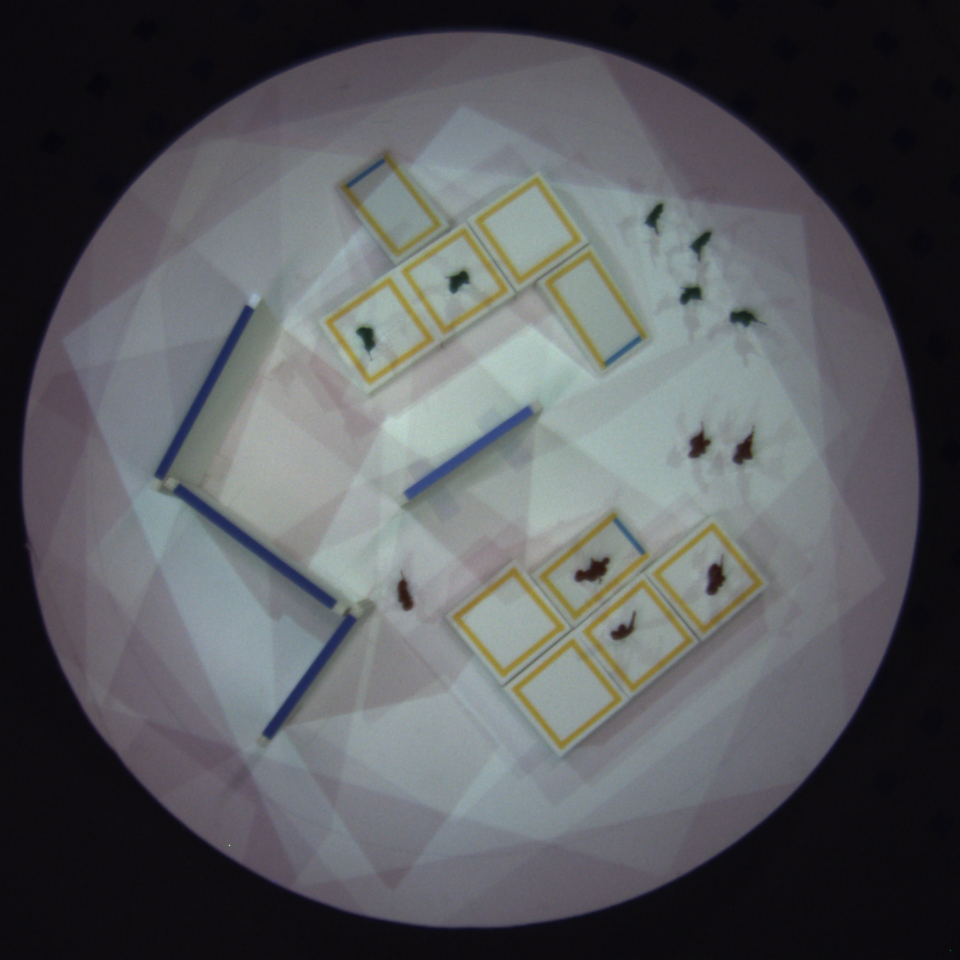
\includegraphics{../gi2012_army/images/raw_with_soldiers.png}}
 \resizebox{!}{\picwidth}{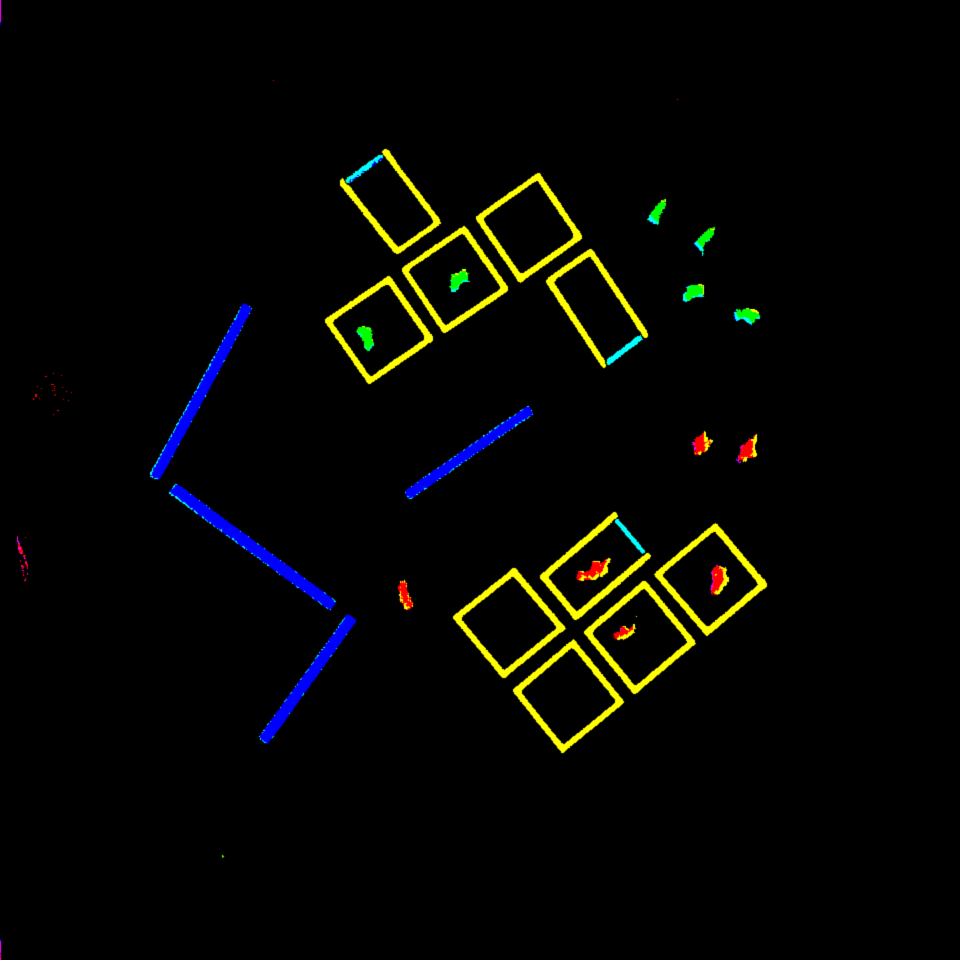
\includegraphics{../gi2012_army/images/enh_colors_with_soldiers_blur.png}}
 \resizebox{!}{\picwidth}{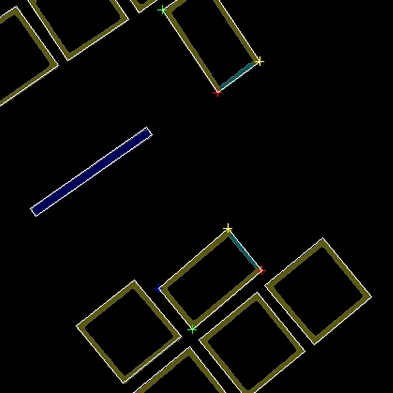
\includegraphics{../gi2012_army/images/terrain_labels_crop.png}}
 \resizebox{!}{\picwidth}{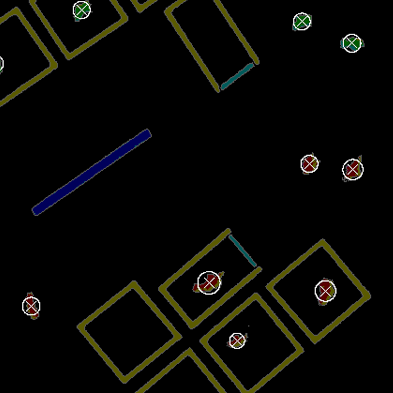
\includegraphics{../gi2012_army/images/labels_with_soldiers_crop.png}}
 \resizebox{!}{\picwidth}{
\includegraphics{../gi2012_army/images/final_heightmap.png}}\vspace{-0.23in}\\
\begin{minipage}{\picwidth}\textcolor[rgb]{1,1,1}{\hspace{-0.05in} {\bf      a)}} \end{minipage}
\begin{minipage}{\picwidth}\textcolor[rgb]{1,1,1}{\hspace{-0.05in} {\bf      b)}} \end{minipage}
\begin{minipage}{\picwidth}\textcolor[rgb]{1,1,1}{\hspace{-0.05in} {\bf      c)}} \end{minipage}
\begin{minipage}{\picwidth}\textcolor[rgb]{1,1,1}{\hspace{-0.05in} {\bf      d)}} \end{minipage}
\begin{minipage}{\picwidth}\textcolor[rgb]{1,1,1}{\hspace{-0.05in} {\bf      e)}} \end{minipage}
\end{center}
\vspace{-0.06in}
\caption[ARmy Object Detection]{a) Raw camera images of the scene show
  variable lighting due to shadows and regions of projector overlap.
  The \emph{vision component} ignores these artifacts by considering
  b) only pixels with highly saturated color properties, which it
  groups into connected components. These components are classified as
  c) quadrilateral terrain regions or d) soldier figurines based on
  size, color, and shape.
e) The final heightfield after dilation and erosion to fill in unwanted discontinuities.}
\label{FIGURE:ARmyObjectDetection}
\vspace{-0.1in}
\end{figure*}



% FIGURE: HEIGHTFIELD OPERATIONS
%\begin{figure*}[t]
%\newcommand{\picwidth}{1.69in}
%\begin{center}
% \resizebox{\picwidth}{!}{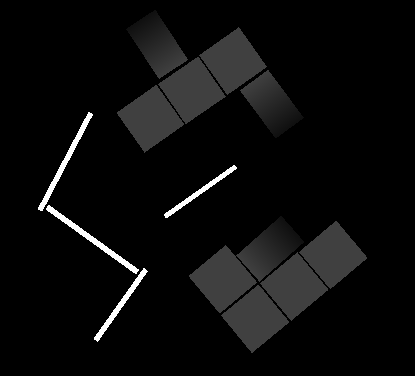
\includegraphics{../gi2012_army/images/initial_heightmap.png}}
%% \resizebox{\picwidth}{!}{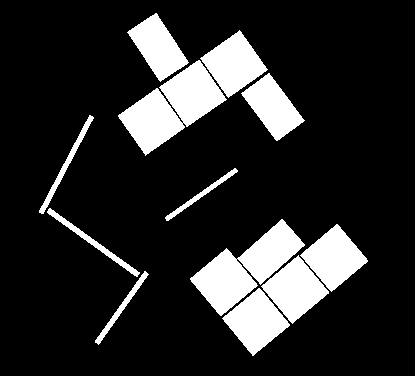
\includegraphics{images/floor_start.png}}
% \resizebox{\picwidth}{!}{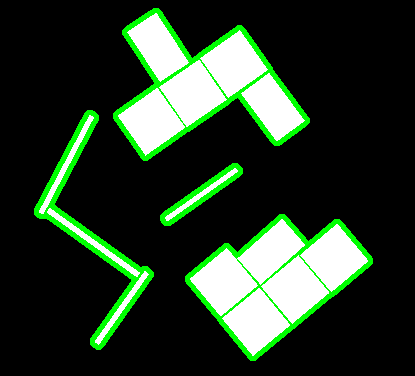
\includegraphics{../gi2012_army/images/floor_dilated_diff.png}}   %\vspace{-1.9in}\\
%  \resizebox{\picwidth}{!}{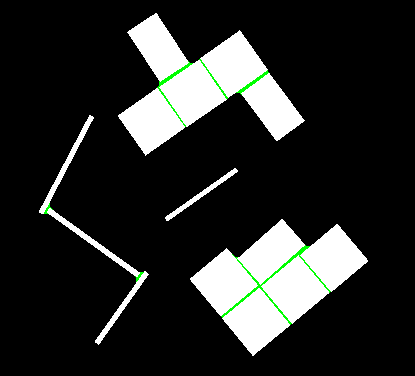
\includegraphics{../gi2012_army/images/floor_final_diff.png}}
%\begin{minipage}{\picwidth}\textcolor[rgb]{1,1,1}{\hspace{0.02in} {\bf        a)}} \end{minipage}
% \begin{minipage}{\picwidth}\textcolor[rgb]{1,1,1}{\hspace{0.02in} {\bf        b)}} \end{minipage}
% \begin{minipage}{\picwidth}\textcolor[rgb]{1,1,1}{\hspace{0.02in} {\bf              c)}} \end{minipage}
% \begin{minipage}{\picwidth}\textcolor[rgb]{1,1,1}{\hspace{0.02in} {\bf              d)}} \end{minipage}
% \end{center}
% \vspace{-0.09in}
% \caption[ARmy Game World Model]{The game world is constructed by
%   beginning with an initial heightfield rendering of the scene (a)
%   and filling in unwanted discontinuities.  
%%First a threshold is
%%   applied (b) to separate the floor from elevated terrain. 
% The next
%   images show the results after dilation (b), and erosion (c), with
%   green regions indicating differences from the original heightfield.
%   These pixels are assigned new height values (d) to form the final,
%   corrected heightfield.}
% \label{FIGURE:HeightfieldOperations}
%\vspace{-0.1in}
% \end{figure*}



%Our SAR tabletop system detects objects using a single calibrated %camera mounted overhead for a top-down viewpoint.  
During acquisition, a single color image from the calibrated overhead camera
(Figure~\ref{FIGURE:ARmyObjectDetection}) is processed by our vision
module, which uses thresholding techniques to identify connected image
components with predominant color attributes matching a set of
identifiable colors. 
% Currently the set is limited to a six color
%vocabulary, including red, green, blue, yellow, cyan, and magenta,
%which has proven sufficient for a number of applications developed
%using the system.
%
%Because the game is designed with the assumption that terrain does %not change beyond the initial setup phase, which occurs before %soldier units have been placed in the scene, the classification rules %can be separated into two distinct sets, allowing the vision module %to operate in separate modes.
%
%After a colored component is detected, 
The vision module classifies each component as one of the known game
object primitives.  During the terrain placement phase, the system
detects the initial configuration of terrain objects, which are
encoded with the colors blue, yellow, and cyan.
%Blue components that fit a rectangular shape within an
%acceptable margin of error are classified as wall objects.  Platform
%objects are detected in the image as yellow components with a valid
%quadrilateral fit.  Similarly, ramps are classified from quadrilateral
%components with three predominantly yellow sides and one predominantly
%cyan side.  The cyan side indicates the low edge of the ramp, which
%reaches down to the table surface.  Once an appropriate quadrilateral
%has been fit to a terrain object, the corners are used to specify
%position and orientation.
%
%After the terrain setup has been finalized, subsequent scene
%recognition steps use the second detection mode, which is responsible
%for identifying soldiers.  
During the army placement and movement phases, the vision module
focuses on appropriately sized red and green colored components that
indicate the location of a soldier figurine.
%s are reserved for
%soldier figurines, any appropriately sized red or green component 
%that falls within an
%acceptable range of sizes 
%is classified as a soldier unit.  Each detected unit is assigned a
%single location equal to the centroid of the component in image space.
%
%Once a component has been classified as a valid object, its known
%world dimensions are used in combination with the calibration data of
%the camera to determine its position and orientation in world space.
%Calibration of the camera and the projectors is performed as a
%preprocessing step~\cite{Zhang2000}.  
Overall, our color-based detection method successfully and robustly
recognizes a variety of objects without the need for large fiducial
markers or embedded sensors, allowing us to easily detect and track a
sizable collection of simple game objects.

%% For any given pixel coordinates in the camera image, the calibration %% parameters define a ray in 3D space representing the corresponding %% path along which light enters the camera.  By using the known height of %% the object at that point, we can backproject along the ray to %% determine the exact world position.

%%  Objects with natural color %% properties, such as brightly colored game pieces, can often be tracked %% without any modification, while objects that lack these properties can %% be tracked with the simple addition of colored markers.

%\subsection{ Virtual Modelling of the Scene}

%As discussed in the system overview, our \emph{world modelling} %component is capable of constructing both 2D and 3D virtual %representations of the physical scene.  The ARmy game application uses

%In order for our system to dynamically project on the detected %objects, it is necessary that we compute a virtual model of the %scene.  This step is handled by a different system component, which %receives the positional data of the detected objects and outputs a %three-dimensional mesh that closely matches the real-world geometry.  %In addition, this module is capable of outputting a two-dimensional %heightfield of the scene, a feature that is utilized by the ARmy game %in order to obtain a simplified representation of the game world.

%\fbox{Mention texture stuff here? Special-case UVs for floor?} \\
%\fbox{Also, does it sound like I'm taking credit for this?}

\vspace{-0.15in}
\paragraph{Modeling the Game World }

%The game world is represented as a two-dimensional heightfield of the %scene, discretized into a high-resolution square grid.

%Once the terrain objects have been acquired, 
The terrain geometry is processed to remove unwanted
discontinuities, such as small gaps between adjacent platforms and
ramps that would undesirably block the movement of units.
%The system computes a two-dimensional heightfield representation of
%the scene.  
%This is
%done by creating a binary image from the heightfield, with foreground
%pixels representing elevated terrain primitives.  Next binary dilation
%and erosion are applied to the image, which fills in unwanted, narrow
%background features.  The new foreground pixels are assigned
%reasonable height values based on their neighbors
%
The resulting heightfield (Figure~\ref{FIGURE:ARmyObjectDetection}e) is used to construct a valid movement
graph
%which the game module uses to approximate the travel distances
for calculation of travel distances
as units move through the scene.  
%Each graph location stores
%the cost of moving from the cell to each of its eight neighbors,
%subject to a maximum height difference threshold.  
Two adjacent pixels are connected only if the difference in height is
less than a prescribed elevation difference threshold.  
%If the difference in height of two adjacent pixels is below the
%elevation difference threshold, then the cells are connect neighbors,
%and the associated movement cost is equal to the Euclidean distance
%between the two. 
%Otherwise the distance is set to infinity.\fbox{needed?}  
%The
%resulting 
%graph reflects movements that are legal according to the
%rules of the game, allowing for units to traverse flat terrain regions
%and gradual elevation changes on ramps, but not to cross sharp
%boundaries, such as cliffs or walls.  Because the terrain
%configuration does not change after the terrain placement step, these
%distance values are computed once at the beginning of the game.

%% Since each cell is connected to at most eight neighbors, the average %% size of the data per cell is invariant with respect to the number of %% cells in the grid, which means that this method scales reasonably to %% higher resolutions.

%% The result of this process is a connected graph that reflects the kind %% of movements expected according to the rules of the game.  Units may %% follow paths that traverse flat terrain regions, as well as ramps, %% which exhibit smooth height variations, but may not pass through sharp %% boundaries, such as cliffs and walls.  More complex movement rules %% could be integrated simply by changing the rules for assigning %% movement distances between neighbors.  For example, we could add a rule %% that soldiers move more slowly when walking up a ramp than when %% walking down one, by assigning costs asymmetrically between connected %% neighbors according to height differences.  The only requirement is a %% means of initializing the heightfield to accurately represent the %% terrain configuration constructed by the players.

%% As mentioned in the system overview, the world modeling component of %% our system is capable of providing a suitable heightfield rendering of %% the scene.  However, initializing the values of the grid from this raw %% heightfield output creates a few problems.  In fact, this height %% information is too accurate, in that it often captures tiny %% discontinuities that players would generally want to ignore.  For %% example, consider two platform objects that are placed side by side %% such that they are nearly touching, with the intention that units be %% able to move freely between the two.  Unfortunately, a thin crevice %% still exists between the two that is likely to be reflected in the raw %% heightfield.  If unaltered, this feature would result in an impassable %% barrier, defeating the intended purpose of the terrain configuration.


%% To solve this problem, I employ a few common image-space techniques to %% fill these unintended gaps.  The steps of this process are shown in %% Figure~\ref{FIGURE:HeightfieldOperations}.  First a threshold is %% applied to the heightfield, such that all pixels with height value %% greater than zero are set to the value of one.  The result is a binary %% image, in which all black background pixels correspond to the base %% height of the table surface, and all white foreground pixels %% correspond to terrain objects of higher elevation.  

%% Next I apply binary dilation and erosion, which in that order comprise %% an operation known in morphology as ``closing.'' Dilation involves %% centering an image kernel, in this case a disc, at each foreground %% pixel and activating the pixels that are overlapped.  This expands the %% foreground regions, filling in tight crevices and other undesired %% features.  Erosion performs another sweep with the same kernel, but %% instead deactivates locations where the kernel overlaps any background %% pixels.  This reduces the foreground components back to their %% approximate original size, but leaves the newly filled features %% intact.

%% Finally, the modified image is compared to the original threshold %% image.  For each newly activated pixel, I assign a new reasonable %% height value equal to that of the nearest nonzero pixel in the raw %% heightfield.  Although the method may sometimes lose minor details, %% such as sharp internal corners, the end result is a heightfield that %% more closely matches expected continuities.

\vspace{-0.15in}
\paragraph{Tracking Soldier Movement }

%When a unit is placed at a given location in the scene, 

To determine each unit's valid movement options, the game module
%the game
%module must determine all possible movement options.  
%
%It does this by
performs
%ing 
a breadth-first search of the movement graph
%across the connected graph,
%enumerating all possible destination points, as well as an estimate of
%the minimum distance required to reach each destination.  The search
%is 
limited by the unit's maximum movement distance.
% of 4''.
%, such that only
%positions reachable by legal movement paths are generated.  
%Our
%current implementation computes the shortest Chebyshev path, \fbox{Reference? also, are we sure about that?} thus our
%movement regions are octagonal in open space.
%
%% The path enumeration algorithm results in movement using grid-based %% distances instead of straight-line Euclidean distances.  Because each %% path consists only of transitions between neighboring grid cells, %% units are effectively restricted to movement along the primary eight %% directions.  To illustrate this, consider a unit standing in a region %% of completely flat terrain with no obstructions, such as the unit at %% the center of the configuration shown in %% Figure~\ref{FIGURE:MovementRegions}.  In a typical miniature war game, %% the unit can move to any point within a surrounding circle of radius %% equal to the maximum movement distance.  However, according to the %% movement rules of the current ARmy implementation, the unit's movement %% is constrained to an octagon, since it may only travel to locations %% reachable by a combination of cardinal and diagonal moves.  Although %% this could be corrected by a more complex pathing algorithm, %% preliminary player feedback has suggested that the octagonal regions %% are acceptable and do not greatly detract from play.
%
%An important detail of the game implementation at present is that the %vision module does not uniquely identify individual soldier units.  %This is a result of the limitations of the vision techniques %currently used, which as previously mentioned, identify objects as %connected components with specified color properties, and are %therefore unable to distinguish between two objects with similar %features.  
%
%With the limited resolution of the camera and the general challenges
%of computer vision, it is not possible to robustly and uniquely
%distinguish the nearly identical soldiers as they are moved across the
%table.  
The player is allowed to simultaneously move any number of his units,
requesting a new scene acquisition only when he would like to see an
updated display or has decided on a final configuration.
Unfortunately, our current tracking method does not uniquely identify
each unit (it only distinguishes red versus green) and we did not
want to limit players to moving a single unit between updates, as this
would disrupt play.
%; however, this would require
%requiring the
%players to pause many times per turn.  
%
%technique is limited by an inability to
%distinguish between objects of similar size, color, and shape, as well
%as infrequent picture updates due to the requirement that users
%withdraw from the table surface during acquisition.  
Thus, the game module must deduce the likely correspondence between
the units' current and previous locations using the Kuhn-Munkres
algorithm~\cite{Kuhn1955,Munkres1957}.
%sometimes known as the Hungarian
%method
%maintain identification of each unit on a
%frame-to-frame basis by relying on temporal coherence alone.
%
%
Given the $m$ 2D locations of 
%representing the configuration of a
a player's units before an update, and a set of $n$ locations
representing the newly detected positions,
% of the units after the
%update.  
we construct a $m \times n$ matrix
$A$, such that each coefficient $A_{ij}$ is equal to the assignment
cost of matching the $ i^{th} $ unit of the old configuration to the $
j^{th} $ unit of the new configuration.  
%In this case, the assignment
The algorithm
%Kuhn Munk
%cost is simply set to the minimum valid movement distance between the
%two positions, as computed by the breadth-first search of the previous
%path enumeration step.  
solves for the minimum cost correspondence between the locations.
%If no valid move exists between the two
%points, either due to impassable terrain or maximum distance
%constraints, then the assignment cost is set to a large value
%representing infinity.
%
%The result of the matching algorithm is a mapping that allows the game
%module to reasonably maintain correct identification of each unit
%across movement frames.  
%Because the algorithm does not require that the two sets be of the
%same cardinality, this method gracefully handles detection errors
%robustly handles 
%error cases in which
%units might have been illegally added or removed from the scene, by
%correctly identifying extraneous or missing units.


%
%The simultaneous movement of multiple units means that at each update,
%the game module must map the last known configuration of units to the
%the newly acquired state, and verify that the changes constitute a set
%of legal moves.  

%k,MunkresCode}.
%  The current
%application uses an existing open-source implementation, written by
%John Weaver and made available for free use under the GNU General
%Public License~\cite{
%


%% Nevertheless, it should be noted that the resultant mapping is not %% always exactly what players might expect.  For example, consider a %% situation in which two units cross paths, such that each ends in a %% location relatively close to the other's starting location.  In this %% situation it is quite likely that the game module will incorrectly %% swap the identities of the two units.  Although this artifact is %% clearly undesirable and may cause potential confusion, it does not %% actually have any consequences on the state of the game, since the %% current prototype assumes that all units are functionally equivalent.  %% However, a more complex set of game rules involving multiple types of %% units with individual state information would obviously require a more %% robust means of identification and tracking.

\vspace{-0.15in}
\paragraph{Line of Sight Calculation }

%As explained in Section~\ref{SECTION:CombatSimulation}, opposing units
%within a 8'' maximum firing radius that have a clear, unobstructed
%line of sight will engage during the combat round.
%
We use the 2.5D heightfield representation of the game world
%; thus,
to perform automatic visibility tests between opposing units.
%performing automatic visibility tests is a relatively trivial matter.
%Given two army unit viewpoints of specified location and height,
%the game module
%simply fits 
%we intersect the 3D line segment connecting these points with the heightfield.
%three-dimensional line between the two, and then
%discretizes the line into segments based on an interval with length
%smaller than the width of a single grid cell.  At each of these
%sampled points, the method verifies that the height of the terrain
%field is less than that of the line.  If no point violates this
%property, then the line of sight is deemed valid.
%\fbox{Too trivial to talk about in such detail?}


\vspace{-0.15in}
\paragraph{Visual Augmentation }


% \begin{figure*}[t]
% \newcommand{\picwidth}{5in}
%\begin{center}
% \resizebox{\picwidth}{!}{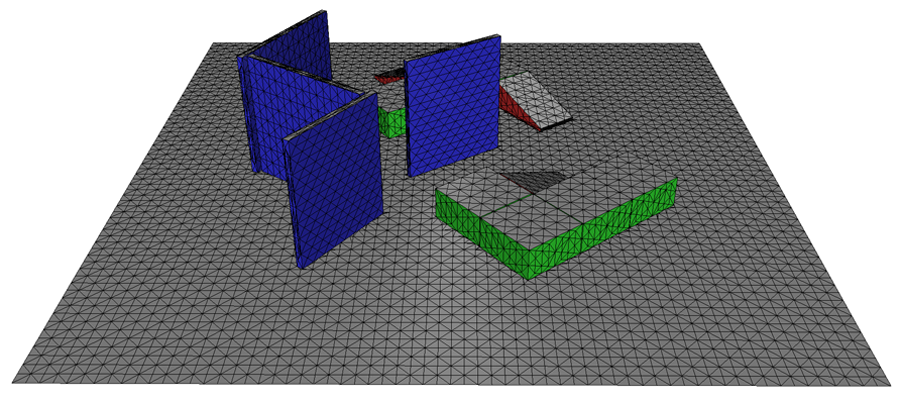
\includegraphics{images/angle2_materials.png}}\\
% \resizebox{\picwidth}{!}{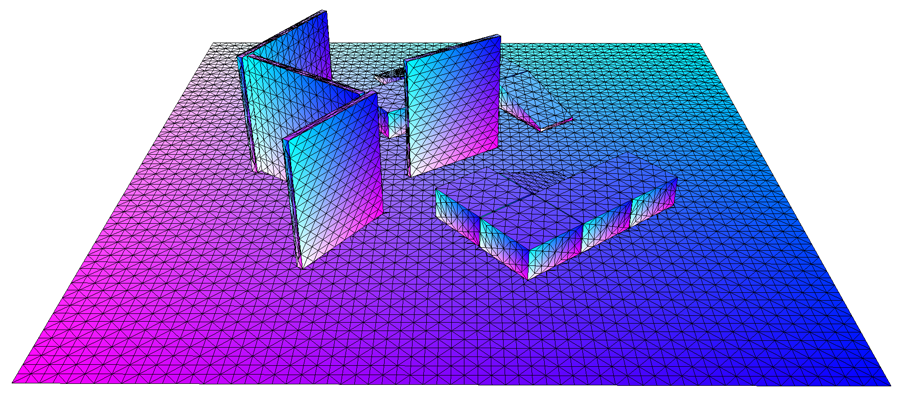
\includegraphics{images/angle2_texture_coordinates.png}}
% \end{center}
% \caption[Assignment of Material Properties]{ The world modeling
%   component assigns material identities to the surfaces of the model
%   according to the needs of the application.  In the top image, the
%   colors represent different material identifiers.  The bottom image
%   is a visualization of the texture coordinates assigned to each
%   surface.  Notice that the top surfaces of platforms and ramps are
%   mapped with texture coordinates aligned with the floor, so that a
%   single continuous texture can be applied.  }
% \label{FIGURE:MaterialProperties}
% \end{figure*}

%The ability to apply virtual textures to specific physical objects and
%surfaces in the scene is a basic primary feature of our dynamic
%projection system.  
The positions and orientations of detected terrain objects are used to
create a virtual 3D mesh representation of the scene.  The ARmy
application generates textures for each of the surfaces in the mesh
and the SAR system coordinates the display of this information into
the scene using the calibrated projectors.

%representation of the scene in the form of a
%three-dimensional mesh with texture coordinates for each surface.
%, which are then used by applications to specify textures
%for display.  In other words, applications use the projection system
%to augment objects by assigning textures to each of the identified
%surfaces.
%(Figure~\ref{FIGURE:MaterialProperties}).
%The ARmy application displays information on the horizontal surfaces
%through a single overlay texture, which is shared by the table surface
%and the top surfaces of all platforms and ramps.  The overlay is of
%the same resolution as the 512$\times$512 heightfield, such that each
%pixel corresponds directly to a single position in the game world.
%Although this resolution is sufficient for covering the 42'' diameter
%table, higher resolutions would improve the quality of the
%visualizations and game play, allowing for smoother textures and more
%detailed display icons.


\section{ARmy Design and Interaction User Study}

%We had several goals in designing the user study for our
%spatially augmented gaming prototype.
The first goal of our user study was to determine if interaction with
the system was natural and intuitive, and to judge the learning curve
for users familiar with physical board games and computers but new to
spatially augmented reality.  A companion goal was to assess the
stability and robustness of our SAR system in
a full game scenario with non-developers.  Most
importantly, we wanted to solicit feedback on the visualization
elements and overall gameplay.  To provide a baseline for comparison,
all study participants played both a traditional, non-augmented
version of the ARmy game as well as the projector augmented game.  We
hypothesized that the augmented version would be less tedious, less
ambiguous or contentious, and that movement and combat would be more
efficient.  Altogether, this would allow users to play more rounds of
the game and explore and evaluate more complex gaming strategies.
% allow users to
%play faster through more rounds of movement and combat, and would
%allow them to experiment with and evaluate different strategies.  
We also hypothesized that users would find the augmented reality
technology more engaging and immersive than the traditional version of
the game.

\vspace{-0.15in}
\paragraph
{Goals for User Study Design}

%To have a fair comparison, 
We designed the study as a direct comparison of the same basic game
played two different ways: using traditional non-augmented technology
(rulers \& dice), and using the projector augmentation.  We held
constant the game rules, including the turn sequence, movement
restrictions, combat sight lines, and combat probabilities.
%
After an introduction to the SAR system and a brief description of the
games rules ($\sim$10 minutes), the participants played the game three
times.  The preliminary game was for practice ($\sim$15 minutes)
in which the participants used {\em both} the traditional mechanisms
of rulers and dice and the projected visualizations of movement areas
and combat circles.  In the practice round each player started with 5
units and we encouraged the participants to set up near their
opponent to ensure they gained experience with the combat rules.  Most
participants played 1 or 2 full cycles of gameplay (movement for each
player and joint combat after each movement phase).
% to familiarize
%themselves with the rules.
%
Next, the participants played two full games, one with and one without
augmentation, in a randomly-selected order.  For each of the full
games, players started with 12 units each and played for a maximum of
20 minutes.  Participants were specifically {\em not allowed} to use
rulers and dice when playing the augmented game.  Similarly, all
projector visualization and texturing was disabled for the
non-augmented version.
%
The supplementary video shows sample footage of both the augmented and
non-augmented versions of the movement and battle phases of the game.
The script (read aloud to participants) for the user study is included
as supplementary material.

\vspace{-0.15in}
\paragraph{Background of Study Participants}

We believe it is important to find participants who enjoy playing
games and have a sense of competitiveness, strategy, and intellectual
curiosity when doing so.
%
Thus, we recruited artists and computer scientists from the Games and
Simulation Arts and Sciences undergraduate major.
%, which consists of
%artists and computer scientists (and dual majors).
%
%
%
%\fbox{can we put this in a table?}
%\fbox{will it make it smaller?}
We had a range of participants from freshmen through graduate
students.  
%
In total, 26 users participated in the initial pilot study (3 females,
5 males) or the main study (6 females, 12 males).  
%We made a few
%revisions to the instructions and questionnaire after the pilot study,
%but the procedure and data collected was similar between the two
%studies.  
We summarize the background for the participants in the main
study: 13 of the 18 participants 
%are studying game design with 
have 0.5-5 years formal education in game studies.  12 of the
participants have at least 3 years formal education in computer
science.  11 of the participants have at least 1 year of formal art
education, 7 have at least 4 years art education.  All users have at
least 3 years experience playing computer games, 14 had more than 10
years experience.  All users have experience playing board games, 15 of
them have more than 10 years experience.  Half of the users had prior
experience (0.5-3 years) with table top games similar to {\em
  Warhammer 40,000}.  
%The varied pool of users provided us with a
%valuable range of feedback from the study.
%\fbox{wording... last sentence necessary?}

\vspace{-0.15in}
\paragraph{Written Questionnaire}

\begin{table}[tb]
\begin{center}
\begin{tabular}{@{}l|c@{~}c|c@{~}c|c@{}}
                & \multicolumn{2}{c|}{{\small non-augmented}} & \multicolumn{2}{c|}{{\small augmented}} & {\small $\Delta$} \\
{\small avg. rating    } & {\small all(18)} & {\small 2$^{nd}$only(10)} & {\small all(18)} & {\small 2$^{nd}$only(8)} & {\small all} \\ \hline
{\small acc. distance  } & \small 3.7 & \small 4.0 & \small 4.5 & \small 4.1 & \small 0.8 \\
{\small acc. sight lines} & \small 3.8 & \small 4.0 & \small 4.8 & \small 4.6 & \small 0.9 \\
{\small acc. rules     } & \small 3.8 & \small 3.9 & \small 4.6 & \small 4.4 & \small 0.8 \\
{\small subjectivity   } & \small 4.1 & \small 3.9 & \small 4.6 & \small 4.6 & \small 0.6 \\
{\small interest       } & \small 3.5 & \small 3.9 & \small 4.6 & \small 4.6 & \small 1.1 \\
\end{tabular}
\end{center}%
\vspace{-0.05in}
\caption{Participant's rating of the accuracy of distance
  calculations, line-of-sight judgments, and implementation of rules,
  their assessment of the subjectivity of rule enforcement, and their
  overall interest while playing the game.  Each is scored on a scale
  of 1 to 5, with 5 being the positive attribute quality.
\label{table:questionnaire}
\vspace{-0.1in}
}
\end{table}

At the end of play, each participant filled out a written
questionnaire (supplementary material)
%.  We asked users to 
directly comparing the augmented and non-augmented versions of the
game 
%by rating on a scale of 1 to 5 
for several important gameplay characteristics
%of the game
%each of the following characteristics of the
%game:
%\vspace{-0.1in}
%\begin{itemize}
%\item 
%the accuracy of distance calculations,
% \vspace{-0.1in}%\\(1=inaccurate, 5=accurate)\vspace{-0.1in}
%\item 
%the accuracy of line of sight calculations for combat,
% \vspace{-0.1in}%\\(1=inaccurate, 5=accurate)\vspace{-0.1in}
%\item 
%the accuracy of game rule implementation,
% \vspace{-0.1in}%\\(1=frequent errors or confusion, 5=no errors or confusion)\vspace{-0.1in}
%\item 
%the subjectivity of enforcement of the rules, and
% \vspace{-0.1in}%\\(1=subjective/some disagreement, 5=no disagreement)\vspace{-0.1in}
%\item 
%their interest level during game play.
%\\(1=tedious or boring, 5=engaging and fun)\vspace{-0.1in}
%\end{itemize}
%
%The results of these ratings are summarized in
(Table~\ref{table:questionnaire}).  The average rating for all 18 study
participants for each version of the game is provided.  We also
separately average the ratings of the users who played that version of
the game as their \emph{second} playthrough (when they were more
familiar with the game mechanics, rules, and strategy). 
% 8
%participants (4 pairs) played the non-augmented version first.  10
%participants (5 pairs) played the augmented version first.
%
Overall, the ratings indicate that participants were interested in
playing both games, thought that the different versions accurately represented the game mechanics,
found enforcement of rules was not too subjective,
felt that the game was fair, and rarely disagreed with each other or
with the computer.  
%The participants did consistently rate the
%augmented version of the system more positively on each
%characteristic.  
Using Single Factor ANOVA, users rated the augmented version 
more positively than the non-augmented with a $p$ value of .005 or lower in every 
case except subjectivity.  Users rated subjectivity higher with a $p$ value of .08.

\vspace{-0.15in}
\paragraph{Timing Results}


A video camera recorded each experiment
%, which allowed us to
%review the timing data for each game.  We 
allowing us to measure the time for terrain setup, initial army
placement, average time for each player's movement phase (red or
green), average time for a combat round, and average time for a battle
(when two units face off, requiring each player to roll once).  We
also counted the number of rounds (red move/combat/green move/combat)
per game, and the number of battles per game
%\fbox{ Is there a better way to explain what a round is?}
(Table~\ref{table:timing_stats}).  This data allows us to compare the
efficiency of play with and without augmentation.  We present the
data averaged over all experiments and a separate average of the games
played as the {\em second} full playthrough.
%, when players are most
%familiar with the game rules and strategy.  
Note: Due to video errors,
a few of the game recordings are incomplete and 
%are thus 
omitted from these averages.

Game setup is slower with the augmented system for both terrain layout
%(100\% slower) 
and unit placement,
% (10\% slower).  
due to a number of minor factors: triggering the remote, waiting for
the visualization to refresh, and reminding players to remove
unnecessary materials from the table and step out of the camera's
field of view.  Similarly, movement phases are slower in the augmented
version because moves are validated by the system and the extra time 
required to correct illegal moves.  With SAR system
overhead optimization we believe these differences can be greatly
reduced or eliminated.  In particular, we believe these improvements
combined with user familiarity with the movement region visualization
will allow movement phases to be faster in the augmented version than
in the non-augmented version.

\begin{table}[tb]
\begin{center}
\begin{tabular}{@{}l|cc|cc@{}}
               & \multicolumn{2}{c|}{\small non-augmented} & \multicolumn{2}{c}{\small augmented} \\
\small averages       & \small all(9) & \small 2$^{nd}$only(3) & \small all(9) & \small 2$^{nd}$only(5) \\ \hline
\small terrain setup  & \small 1:16    & \small 1:13         & \small 2:46    & \small 2:07         \\
\small army placement & \small 2:52    & \small 2:38         & \small 3:03    & \small 3:11 \\ 
\small movement phase & \small 0:42    & \small 0:36         & \small 0:52    & \small 0:47 \\
\small combat phase   & \small 1:33    & \small 2:13         & \small 0:22    & \small 0:18 \\
\small single battle  & \small 0:16    & \small 0:21         & \small 0:04    & \small 0:03 \\ \hline
\small \# rounds per game & \small 2.3  & \small 2.0         & \small 3.9     & \small 4.1 \\
\small \# battles per game & \small 26.1   & \small 24.5   & \small  36.6    & \small 41.0 
\end{tabular}
\end{center}%
\vspace{-0.05in}
\caption{ The average timing data (minutes:seconds) for various stages
  of play are summarized for both non-augmented (traditional) and
  SAR augmented experiments.
\label{table:timing_stats}
}
\vspace{-0.1in}
\end{table}

Not-surprisingly, the augmented system's main efficiency improvement
is gained in the combat simulation phase ($\sim$4X faster).  The
simulation of each battle is visualized one-at-a-time for the players
($\sim$1 second per virtual ``die'' roll).  Note that the combat phase
also includes removal of disabled units.
% at the end of the phase.
The greatest efficiency improvement is in calculating which units have
line of sight and are in range, and {\em most importantly}, in keeping
track of which battles have occurred and correctly accounting for all
combinations of opposing units when they are densely clustered.

As we hypothesized, overall the augmented version allows players to
complete more cycles of play before time is called (60\% more),
and similarly, more total battles are fought (40\% more) in the
augmented version.

\vspace{-0.15in}
\paragraph{Quantitative Analysis of Unit Movements}



Next, we analyzed the unit movements in augmented games.  We
were interested in quantifying the fraction of unit movements that
were close to the maximum 4'' distance.  We also examined
all cases in which a unit was moved slightly beyond this maximum distance
and marked as an illegal move.  Table~\ref{table:movement_data}
summarizes the data for a total of 678 unit movements.
%
60\% of unit movements were ``big moves'', reaching more than 75\% of
the maximum distance and 25\% of the moves pushed within a pixel of
the 4'' movement radius.  We assume that for most of these moves the
user was strategically interested in maximizing unit movement.
However, they may have shied away from making a full 4'' movement to
avoid having that move marked as illegal.  9 out of 14 pairings saw
at least one borderline unit movement marked as illegal during either
the practice round or the full game.  When a movement
is marked illegal,
%as a borderline illegal movecheat,
it causes an interruption in game flow, requiring correction of the
error.  In most cases, the player over-corrected for the error,
backing up the soldier to approximately 75\% of the full move.  In a
few cases, the player was confused about which unit moved too far, and
conservatively adjusted several other {\em legal} moves.

Only twice during our study did the system catch flagrantly
illegal moves, and neither case was malicious.  In one instance the
illegal move came in the confusion immediately after a detection
error.  We found that detection errors during play were rare,
proving that our prototype system is robust, engaging, and thoroughly
playable.  Detection errors occurred when units were placed too
close together and detected as a single unit,
% a unit was missed (color threshold),
%red vs. green units were mislabeled 
%mis-recognized red vs. green unit, 
when a unit hidden behind a wall was not visible to the camera,
and a few rare color thresholding errors.
%person was not visible (behind a
%wall).  
Other detection errors were related to game rule ambiguities; for
example, straddling a unit between platforms that touch only at the
corner or balancing units on the very edge of a platform.


\begin{table}[tb]
\begin{center}
\begin{tabular}{@{}l@{~~~~~~~~~}r@{~}r|@{~~~~}r@{~~~}r@{~~}c@{}}
                      & \multicolumn{2}{l|@{~~~~}}{\small practice} & \multicolumn{3}{c}{\small full games (14)} \\ \hline
%\small \# games              &     &                         & \small 14   & &     \\
\small total \# moves        & \small 141 &                                & \small  537 & &  \\
%\small avg. moves / player   & \small   5 &                                & \small 19  & &  \\
%moves $<$ 75\%       &  51 & 36\%                    & 222 & 41\% &  (7-70\%)  \\
\small moves $>$ 75\%        &  \small 90 & \small 64\%                    & \small 315 & \small 59\% & \small (30-93\%)  \\
\small moves $>$ 95\%        &  \small 44 & \small 31\%                    & \small 127 & \small 24\% & \small  (0-63\%)  \\
\small borderline illegal    &  \small 8  &                                & \small  4  & &  \\
\small flagrant illegal      &  \small 0  &                                & \small  2  & &  \\
\small detection errors      &  \small 4  &                                & \small  8  & &  \\
\end{tabular}
\end{center}%
\vspace{-0.05in}
\caption{A summary of the individual ARmy unit movement data for the
augmented gameplay during both practice and full games.
%the
%  augmented version of game play.
\label{table:movement_data}
\vspace{-0.1in}
}
\end{table}




\vspace{-0.15in}
\paragraph{Verbal and Written Feedback}

We encouraged participants to 
%to each other and the
%experimenters, 
ask questions and offer feedback throughout the study.  
Each
participant also answered
%completed the written questionnanswered 
several short written answer questions.
% giving us further insight about the positive and
%negative aspects of each game mode.  
%
A summary of the participant comments:
%^Many participants had the same general comments about the games.  A
%^summary of these comments:

%\Vspace.18in}
%\newcommand{\mysep}{-0.08in}

%\begin{small}
{\em Positive Aspects of Traditional Game:} %, Non-Augmented Game:}
%
%\begin{itemize}
%
%\vspace{-0.05in}
%
%\item 
%felt like traditional board game
``It was a little more hands on'' and
``player decisions were more fluid'', which
``keeps players actively involved in game play''.
%\vspace{\mysep}
%
%\item 
Tactile control allowed participants to ``know exact outcome of dice''
and they ``felt responsible for the outcome of the
dice''.
%\vspace{\mysep}
%
%\item 
Users appreciated the
%wiggle room in interpretation of the ryles
``slight bending of rules for more realistic and entertaining game play''.
%it was easier to do certain things, like skip a turn or make mutual agreements on rulings or confusion


%being able to check whether you were in range without waiting for the system to update
%not having to worry about glitches

%\end{itemize}

%\vspace{-0.18in}
{\em Negative Aspects of Traditional Game:} %, Non-Augmented Game:}
%
%\begin{itemize}
%
%\vspace{-0.05in}
%
%\item 
%time consuming
%measuring is tedious
``Much slower combat (actually rolling the dice each time and making sure every combination of soldiers is accounted for)''
%dice kept falling off table 
and
``when many attacks [happened] at the same time, it made the game stop and not be fun''.
%\vspace{\mysep}
%
%\item 
%difficult to keep up with everything during combat
``In a dense soldier cluster there were so many attacks made that we probably lost count at some point and either attacked too many times or too few''.
%``a slightly sloppy feel where i felt that i could be making mistakes''
%sometimes it was tricky remembering which pairs of soldiers had already fired, but we came up with a strategy that mostly solved that.
Participants experienced ``occasional confusion (even about whose turn it was)''
%\vspace{\mysep}
%
%\item 
%some subjectivity with measurements
and ``While we made decisions, they were not necessarily the
correct ones in terms of the rules''.

%\end{itemize}

%\vspace{-0.18in}
{\em Positive Aspects of Augmented Game:} %Game with Projection Augmentation:}
%
%
%\begin{itemize}
%
%\vspace{-0.05in}
%
%\item
Participants found that the ``visualizations were easy to understand'',
it was
%can see where you're going
``easy to see how far you can move'',
%distances were clearly marked as well as line of sight and current shooting pairs.
and it was ``never unclear about whose turn it was or what could be done''.
%``no questioning who was on higher ground''
%\vspace{\mysep}
%
%\item 
%didn't have to do any work
Most participants ``trust [the] computer'' and the games had
``no disagreement between players since there was an ultimate referee''.
%no human errors
%it fixed the "wait did he shoot yet?" problem.  
%\vspace{\mysep}
%
%\item 
%projected scenery made me feel like i was playing a game and not a probability simulator
%visually it was far more interesting
The use of projective texture was  ``more visually stimulating''
and the animations of
``the arrows for combat were amusing to watch''.
%\vspace{\mysep}
%
%\item 
Participants specifically commented that faster, more
efficient play made it ``much easier to establish movement strategy''
%combat was faster
%considerably quicker pace
because ``it allowed you to focus on the game play and not the math
behind it''.

%\end{itemize}

%\vspace{-0.18in}
{\em Negative Aspects of Augmented Game:} %Game with Projection Augmentation:}
%
%
%
%\begin{itemize}
%
%\vspace{-0.05in}
%\item 
``Turns were slow'' while ``waiting for recalculation'' and
  ``moving pieces slightly out of range made it take longer
  sometimes''. 
%\vspace{\mysep}
%
%switching between turns was a little slow.
%
%\item
Occasional system glitches and the ``restriction in terrain placement because of projection'' were negatives.
% (vision)
%minor issues identifying scenery
%some setup bugs
%occasional glitches
%things not getting detected for being in certain positions
%wall blockage issue with camera, couldn't move too close to walls.
``Blind spots forced us to simplify our first terrain design a bit.''
%but that's a natural consequence of using a single camera''.
%\vspace{\mysep}
%%
%\item
Explanation of game results was sometimes unclear:
``Don't know the reason the soldier was disabled''.
%\vspace{\mysep}
%
%\item
``Took the player engagement away a bit.  Watched action happen rather
than rolling the dice.  Takes away your feeling of involvement.''
%hard to see line of sight sometimes

%some rules implemented questionable
%\end{itemize}

%\end{small}
%
%\fbox{scalability of color tracking}%
%
%\fbox{* if want more primitives will color tracking work?}
%
%\fbox{Need to better discuss user study data}
%
%\fbox{need to discuss why efficiency is important}


\section{Discussion and Conclusions}
%: Suggestions for Designing Spatially Augmented Games}

%Using a single camera and six projectors, 
Using affordable, off-the-shelf hardware we created an immersive SAR
game experience that 15 out of 18 participants preferred over the
non-augmented version.  Two preferred the non-augmented version and
one person called it a tie.
%a clear majority of users preferred to the
%non-augmented version.  
%With the advent of cheaper projectors and
%cameras, 
We believe that many other physical board and card games could
similarly be positively augmented and improved by such a setup.  
%
Depending on the system budget and physical game environment and
components, this infrastructure could be simplified to use a single
projector or expanded to use multiple cameras or alternate tracking
technology (Section~\ref{section:related_work}).  This system is
practical for installation in home ``game room'' environments.
% While our system was able to
%detect our primitives using a single color camera, a system with more
%complex primitives or requiring full 3D reconstruction could benefit
%from multiple cameras or a depth camera.  
%Recent work has even made
%the possibility of using multiple Kinects together to interpret 3D
%scenes~\cite{Maimone12}.  
%Similarly, while our system has 6 projectors
%many applications, such as ones without large occluding walls, could
%be adequately projected by one or two projectors.


Augmented gaming systems should facilitate and encourage users to make
optimal decisions; for example, in ARmy this often means making a full
4'' distance movement.
%Users should also be encouraged to make the most
%effective moves possible.  
Unfortunately, we found that some users were reluctant to make maximal
movements because the delay in correcting an overmove interrupted game
play.
%the system
%often shyed away from
%making the largest moves after being corrected for moving too far.
Instead of forcing users to nudge pieces back, the system could
automatically recognize these slight over-movements, and clamp the
internal representation of the unit's position to the maximum
distance.
%and
%smooth game flow.
%adjust
%the
%Rather than simply
%telling users to correct their moves we plan to modify the system so
%that a piece is automatically moved back to the farthest allowed move.
We recommend that similar tolerances be incorporated when possible in
all AR based games.
%similarly providing some functionality for maximal
%movement in turn-based movement games

Users were excited by the system ease-of-use and efficiency 
of the battle rounds.
%quickly
%battle rounds went.  
%While the battle rounds went very quickly, 
Game setup 
occasionally 
took longer when technical problems occurred
with the prototype SAR system.  These system issues must be resolved
prior to commercialization of this type of technology.
%While users tend to be
%forgiving if they see parts of the system that save time or look
%exciting, care should be taken to always minimize bottlenecks.
It is important that users feel engaged and in control while 
%using SAR systems and
playing SAR games.
%involved with the system.
Even though the combat rounds were more efficient in
%While the time the battles took in 
the augmented version,
% was four
%times faster, 
some users wished they had more control over the automated battle
sequences and dice rolls.
%We have considered limiting how many battles occur between user
%interactions.  
Future studies are needed to determine
the optimal timing of user interactions and automated system computation.
%to see how long is optimal between user
%interactions should be done.  
More visualization of the simulated die rolls and the ability to specify individual attacks instead of fully automated combat
%pause
%interrupt
%We have considered showing the simulated
%die rolls, or allowing movement at some point midway through 
%long battle sequences
may be beneficial.  Some users noted that the
game state could change significantly between turns.  It was not
uncommon for one half of an army to be eliminated in a single 
%particularly
%intense 
combat round.  More complexity in the game rules, for example ``hit points'' for each unit
would make the game more interesting and require more strategy.
%One potential way to alleviate this would be to have hit
%points or require it to take more than one shot to kill an enemy
%soldier.

%Finally, we suggest having a state diagram that fully encompasses user
%interaction.  This enables fairly accurate predictions of parts of the
%game where there will not be enough user interaction or where there
%may be too much user input before any exciting augmentation.

%\section{Conclusions and Future Work}
%\fbox{I put the negative first}


%\paragraph{Future Work}

%Our SAR system would benefit from 
%several specific improvements, many
%of which point to interesting avenues of future research. 
By adapting our SAR framework to facilitate
%One significant improvement would be to incorporate a method for
simultaneous acquisition and display, the gaming module could more
naturally react
%allowing for the system to react
to users without the need for turn-based update requests.
%A more sophisticated tracking scheme could also lead to improved
%object identification. 
Gesture-based or verbal speech controls, could also be beneficial.
%This part is new
Gameplay could be made more engaging by improvements to the detection
sequence and in finding ways for users to interact during combat.
%
%Similarly, we believe users would feel greater freedom if we provided a method
%for them to make the maximal moves without requiring adjusting and removing 
%if they went over the movement threshold.
%end newpart
Finally, play could be enhanced by displaying state information
directly onto the units to remove clutter, and by adding audio
elements to increase the immersive feel of the game.

Overall, the ARmy application is a fully functional prototype that
demonstrates the key benefits of SAR for tangible gaming.
%and shows how a tangible tabletop
%interface can be combined with a video game module to create an
%entertaining user experience.  
The results of our user study indicate a general participant
preference for the augmented version of our game prototype, and
feedback has shown a positive opinion about SAR technology in the
context of tabletop games.



{\footnotesize
\bibliographystyle{ieee}
\bibliography{army}
}


\end{document}
